\documentclass[11pt,b5paper]{book}
%Deep Learning Based Traffic Vehicle Detection: YOLO with ORB to Push Performance and Their Comparison with some High Speed Models.

\usepackage[utf8]{inputenc}

\usepackage{graphicx} % [draft]{graphicx} to remove all images
\graphicspath{{images/}}
\usepackage{wrapfig}
\usepackage{bbm}

\usepackage{breakcites}

\usepackage[strict]{changepage} % for CV. As the "section" of bch font is slightly off the balance compared with "main text" of crimson font. the balance is then fixed by placing the bch font in the main text, and the "section" of bch font is adjusted accordingly.

%=======================================================================
%%% thesis geometry

\usepackage[text={115mm,197.2mm},hmarginratio=1:1,vmarginratio=1:1,marginparwidth=12mm]{geometry} 

%=======================================================================

\usepackage{lipsum} %generating lorem ipsum

\usepackage{amsmath,amssymb,amsfonts}

\usepackage{setspace}
\usepackage{booktabs}

\usepackage{emptypage} %remove header, footer along with the page number in an empty page
\newcommand\mybar{\kern1pt\rule[-\dp\strutbox]{1pt}{\baselineskip}\kern1pt} %vertical bar
\usepackage{pdfpages} %[draft]{pdfpages} to remove all pdf

\usepackage{float} %force image position

\usepackage{url}
\urlstyle{same}

\usepackage[super]{nth}

\usepackage{textgreek}

\usepackage[hang,flushmargin]{footmisc}
\renewcommand*{\footnotelayout}{\scriptsize}

\usepackage{multirow}

\usepackage[many,listings]{tcolorbox} % color box surrounding anything

%=======================================================================
%%% Minimize overfull hbox output problem

\usepackage{microtype}

%=======================================================================
%%% Abbreviations and add this section to table of contents

\usepackage{multicol} % multicolumns

\usepackage[intoc]{nomencl}
\usepackage{ifthen}
\setlength{\nomitemsep}{-2pt} % this modifies item vertical separation
\setlength{\nomlabelwidth}{1.6cm} % this modifies label horizontal separation; {2.5cm} for single column; {1.8cm} for two column, long acronyms

%%% Grouped multi-column nomenclature %%%

\makenomenclature

\setlength{\columnsep}{1.67pc} % column separation

\makeatletter
\newif\if@nomlist

\newcommand*\nomlist{%
  \@nomlisttrue
  \list{}{%
    \labelwidth\nom@tempdim
    \leftmargin\labelwidth
    \advance\leftmargin\labelsep
    \itemsep\nomitemsep
    \let\makelabel\nomlabel}}

\renewcommand*\thenomenclature{%
  \@ifundefined{chapter}%
    {\section*{\nomname}\if@intoc\addcontentsline{toc}{section}{\nomname}\fi}%
    {\chapter*{\nomname}\if@intoc\addcontentsline{toc}{chapter}{\nomname}\fi}%
  \nompreamble
  \@nomlistfalse
}

\renewcommand\nomgroup[1]{%
  \if@nomlist\endlist\end{multicols}\fi
  \ifx#1A\relax % "1A" can't be replaced with "1a". "a" is fine though in the nomenclature.tex
    \def\nomgroupname{\textbf{Acronyms}}%
  \else
    \ifx#1B\relax % "1B" can't be replaced with "1b". "b" is fine though in the nomenclature.tex
      \def\nomgroupname{\textbf{Roman symbols}}%
    \else
      \def\nomgroupname{\textbf{Greek symbols}}%
    \fi
  \fi
  \begin{multicols}{2}[\raggedcolumns\noindent\textbf{\hspace*{-1pt}\fontfamily{bch}\selectfont\scshape\small{\nomgroupname}}]
  \nomlist
}

\renewcommand*\nompreamble{}
\renewcommand*\nompostamble{\end{multicols}}
\makeatother

%=======================================================================
%%% Modifying the listing items

\usepackage{enumitem}  
\usepackage{pgfornament}
\usepackage{adforn}

%=======================================================================
%%% Unique colors used in this PhD thesis
\usepackage{xcolor}
\definecolor{sophia}{RGB}{125,0,45}
\definecolor{ntnu}{RGB}{0,80,158}
\definecolor{heidelberg}{RGB}{0,65,120} % 

\usepackage{colortbl} % coloring the table
\definecolor{Gray}{gray}{0.9}
\definecolor{White}{RGB}{255,255,255}

% for abstract in chapters 5-9
\definecolor{abstractback}{RGB}{255,248,220}

\definecolor{Test}{RGB}{231,231,231} % must be CAPITALIZED!!!
\definecolor{Test3}{RGB}{128,128,128}
\definecolor{Black}{RGB}{0.0, 0.0, 0.0}
% for figure & table captions, marginnote, etc

\newcommand{\sophia}[1]{\textcolor{sophia}{#1}}
% too late, only used in Acknowledgement

%=======================================================================
%%% hyperref

\usepackage[backref=page]{hyperref}

\hypersetup{
    hidelinks,
    colorlinks=true,
    linkcolor=ntnu,
    citecolor=ntnu,
    urlcolor=ntnu,
    breaklinks,
    linktocpage % for TITLETOC: need to use this to make page number, not text be linked (automatically colored to "ntnu"). if this option is not used, then any text in toc or lof can't be customized in TITLETOC.
}

% === back references == 

\newcommand{\citedbox}[1]{%
  \begingroup\setlength{\fboxsep}{1pt}% 1pt is the default value; height
  \colorbox{White}{\hspace*{-1pt}\vphantom{Ay}#1\hspace*{-1pt}}% each 2pt is the default value; width
  \endgroup % originally the colorbox is set to "Test". it is good, but draws too much attention.
}

\usepackage{etoolbox}

\def\backref#1{{\citedbox{\textcolor{Test3}{Cited on page/s} #1\textcolor{Test3}{.}}}} % use this when \citedbox command is used. 

% === \ref = \autoref == %

%% to make the word "Figure" clickable in addition to its number label
\makeatletter
\renewcommand{\p@figure}{\figurename\ }
\makeatother

%% to make the word "Table" clickable in addition to its number label
\makeatletter
\renewcommand{\p@table}{\tablename\ }
\makeatother

% === explicitly mention the Section name === %

\newcommand*{\fullref}[1]{\hyperref[{#1}]{\autoref*{#1} \nameref*{#1}}}

\renewcommand{\sectionautorefname}{Section}

% ======================== %

%%% Capitalize [C]hapter, [S]ection and [S]ubsection in \autoref (default is not capitalized)

\newcommand{\Autoref}[1]{%
  \begingroup%
  \def\chapterautorefname{Chapter}%
  \def\sectionautorefname{Section}%
  \def\subsectionautorefname{Subsection}%
  \autoref{#1}%
  \endgroup%
}

%=======================================================================

\usepackage{bookmark} % Adding package bookmark improves bookmarks handling, and enable \pdfbookmark for TOC in the main.tex.

% add #(number) in front of the chapter title when it is exported to pdf

\bookmarksetup{numbered}

\makeatletter
\bookmarksetup{%
  addtohook={%
    \ifnum\toclevel@chapter=\bookmarkget{level}\relax
      \renewcommand*{\numberline}[1]{#1. }%
    \fi
  },
}
\makeatother

%=======================================================================
%%% Fonts used in this PhD thesis

\usepackage[T1]{fontenc}

\usepackage{csquotes}
\usepackage[english]{babel}

%% serif, as a main font %%
\usepackage{crimson}

%% sans serif, as decoration %%
\usepackage{roboto} %figure caption fonts

% math font
\usepackage[libertine]{newtxmath} 

% calligraphical font
\usepackage{calligra}

% hiragana/kanji
\usepackage{CJKutf8}

%=======================================================================
%%% Placing any extra information on the margin of the page

\usepackage{marginnote}

\renewcommand{\marginfont}{\fontsize{6.97}{6}\selectfont\roboto}

\newcounter{mynote}% a new counter for use in margin notes
 
\newcommand{\mynote}[2][0]{% a simple margin note
    \refstepcounter{mynote}% step counter
    \mbox{\textcolor{Test3}{\textsuperscript{\themynote}}}% the number (superscript) in text
    \marginnote{\mbox{\textcolor{Test3}{\textsuperscript{\themynote}}}\hspace{0pt}#2}[#1\baselineskip]% the note
    % \marginnote{\mbox{\textsuperscript{\themynote}}\color{sophia}\hspace{0pt}#2}[#1\baselineskip]% the note
}

\newcommand{\mynoteref}[2][0]{% a simple margin note
    \marginnote{\hspace{0pt}#2}[#1\baselineskip]% the note
}


% coloring the page number (referencing) in the copyright
\newcommand{\colpageref}[1]{{\hypersetup{linkcolor=sophia}{\pageref{#1}}}} % or \autopageref

% coloring the word "page" (referencing) in the copyright
\newcommand{\pcol}[1]{{\textcolor{Test3}{#1}}}

% to have a shortcut for coloring the caption, e.g., a, b, c, etc
\newcommand{\capcol}[1]{{\textcolor{ntnu}{#1}}}

%=======================================================================
%%% Bibliography at the end of each chapter, based on NATBIB

\usepackage[super,comma,sort&compress]{natbib} 

\usepackage{bibentry}

\usepackage[sectionbib]{chapterbib} % put ref at the end of each chapter. however, the spacing in the TOC will be messed up. it can be fixed using "numbib" option as shown below
\usepackage[nottoc,numbib]{tocbibind} % numbib (for numbering reference section) is used to enable cross-ref with TOC

\usepackage{hypernat} % to fix the missing page citation "\usepackage[backref=page]{hyperref}" that is nested in between, e.g., 19 is not missing if the refs is from 18-20, i.e., "sort&compress" in natbib is activated

\addto{\captionsenglish}{% if BABEL is used
  \renewcommand{\bibname}{References}
}

\renewcommand*{\bibfont}{\footnotesize}

\setlength{\bibsep}{0.7pt}

%=======================================================================
%=======================================================================
%=======================================================================
%%% Header (and/or footer)
%=======================================================================
%=======================================================================
%=======================================================================

\usepackage{fancyhdr}
\pagestyle{fancy} % this must be placed as a general. DON'T REMOVE IT!

%% with number in front of the title
\renewcommand{\chaptermark}[1]{ \markboth{Chap. \thechapter\ \ \enspace #1}{} } %\chaptername or "Chap."
\renewcommand{\sectionmark}[1]{ \markright{\thesection\ \ \quad #1} }

%==========================================================================%
%=================== header style for regular section =====================%
%==========================================================================%

\newcommand\headerregularsection{

    \pagestyle{fancy} % optional, but I place this here anyway
    \fancyhf{}

    \fancyhead[LE]{\leavevmode\llap{\textbf{\fontfamily{ppl}\selectfont\footnotesize\thepage} \ \hspace{1mm} \textcolor{sophia}{$\blacktriangleright$} \hspace{2mm}}{\scriptsize\bfseries\fontfamily{bch}\selectfont\scshape\leftmark}} % default font is Crimson for page number and Charter "bch" for the rest

    \fancyhead[RO]{{\scriptsize\bfseries\fontfamily{bch}\selectfont\scshape\rightmark}\rlap{\hspace{2.0mm} \textcolor{sophia}{$\blacktriangleleft$} \hspace{1mm} \ \textbf{\fontfamily{ppl}\selectfont\footnotesize\thepage}}} % default font is Crimson for page number and Charter "bch" for the rest

}

\setlength{\headheight}{13.6pt} % remove headheight error message: https://tex.stackexchange.com/questions/271159/turn-off-fancyhdr-auto-spacing, https://latex.org/forum/viewtopic.php?t=30693 

\renewcommand{\headrulewidth}{0pt}

%==========================================================================%
%=================== footer style for new chapter page ====================%
%==========================================================================%

\fancypagestyle{plain}{% % this command to set aside every new chapter to be different
    \fancyhf{}%
    \rfoot{\mypage} % draw box surrounding page
    \newcommand\mypage{%%
        \raisebox{6pt}[0pt][0pt]{%% {Xpt}[Xpt] determines the +y,-y both for the box AND the page number
        \color{ntnu}
        \rule[-1.5ex]{2.5cm}{0.5pt}%% [Xex]{Xcm}{Xex} are y position, the length of the box, work only with positive number and height of the box
        \hspace*{-2.0cm}%% box coordinate, right side
        \makebox[0pt]{\textcolor{ntnu}{\fontfamily{ppl}\selectfont\bfseries\footnotesize\thepage}}%% % page number properties ;  % default font is Crimson for page number and Charter "bch" for the rest
        \hspace*{0.5cm}}%% box coordinate, left side [BETTER not to change this]
    }        
    \fancyfootoffset{1.35\marginparwidth} % give offset to page number
}

%==========================================================================%
%========= header style for special section (a.k.a. REFERENCES) ===========%
%==========================================================================%

\newcommand\headerspecialsection{%
    \pagestyle{fancy} % fancypagestyle{CUSTOM_NAME}{} only work in the first page
    \fancyhf{}
    \fancyhead[LE]{\leavevmode\llap{\textbf{\fontfamily{ppl}\selectfont\footnotesize\thepage} \ \hspace{1mm} \textcolor{sophia}{$\blacktriangleright$} \hspace{2mm}}{\scriptsize\bfseries\fontfamily{bch}\selectfont\scshape\nouppercase\leftmark}} % default font is Crimson for page number and Charter "bch" for the rest

    \fancyhead[RO]{{\scriptsize\bfseries\fontfamily{bch}\selectfont\scshape\nouppercase\rightmark}\rlap{\hspace{2.0mm} \textcolor{sophia}{$\blacktriangleleft$} \hspace{1mm} \ \textbf{\fontfamily{ppl}\selectfont\footnotesize\thepage}}} % default font is Crimson for page number and Charter "bch" for the rest
} 

%============================================================================%
% header style for special section for appendix with section/subsection(e.g. B) %
%============================================================================%

\newcommand\headerspecialsectionappendix{%
    \pagestyle{fancy} % fancypagestyle{CUSTOM_NAME}{} only work in the first page
    \fancyhf{}
    \fancyhead[LE]{\leavevmode\llap{\textbf{\fontfamily{ppl}\selectfont\footnotesize\thepage} \ \hspace{1mm} \textcolor{sophia}{$\blacktriangleright$} \hspace{2mm}}{\scriptsize\bfseries\fontfamily{bch}\selectfont\scshape\leftmark}} % default font is Crimson for page number and Charter "bch" for the rest

    \fancyhead[RO]{{\scriptsize\bfseries\fontfamily{bch}\selectfont\scshape\leftmark}\rlap{\hspace{2.0mm} \textcolor{sophia}{$\blacktriangleleft$} \hspace{1mm} \ \textbf{\fontfamily{ppl}\selectfont\footnotesize\thepage}}} % default font is Crimson for page number and Charter "bch" for the rest
} 

%==========================================================================%
%====================== footer style for part page========================%
%==========================================================================%

% % FSFPP#1

\fancypagestyle{partpagestyle}{
    \fancyhf{}%
    \rfoot{\marker} % draw box surrounding page
    \newcommand\marker{
        \raisebox{6pt}[0pt][0pt]{%% {Xpt}[Xpt] determines the +y,-y both for the box AND the page number
        \color{white}
        \rule[-1.5ex]{14.6cm}{0.5pt}%% [Xex]{Xcm}{Xex} are y position, the length of the box, work only with positive number and height of the box ; 1st value: [13cm] 
        \hspace*{-2.0cm}%% box coordinate, right side
        \makebox[0pt]{\textcolor{white}{\fontfamily{ppl}\selectfont\footnotesize\thepage}}%% % page number properties ;  % default font is Crimson for page number and Charter "bch" for the rest
        \hspace*{0.5cm}}%% box coordinate, left side [BETTER not to change this]
    }        
    \fancyfootoffset{1.35\marginparwidth} % give offset to page number
}

%=======================================================================
%=======================================================================
%=======================================================================
%%% Part, chapter, section and subsection titles
%=======================================================================
%=======================================================================
%=======================================================================

\usepackage{titlesec} % put [explicit] before {titlesec} if you want to use "Linking the section titles to the ToC, alternative 2"

%=================== style 3c

%=======================================================================

%%% Linking the section titles to the ToC, alternative 4  >>> WORKING PROPERLY (THE BEST)

% % works like a charm
% % this meant to be paired with the chapter, section and subsection styles below (after alternative 5)

% %%% used with alternative 5, since "part page" linking in that alternative works
% %%% also chapter* can't be recognized

\makeatletter

\let\hypersection\section
\def\section{\@ifstar\starsection\mysection}
\def\starsection{\hypersection*}
\newcommand{\mysection}[2][\@empty]% #1=optional (toc and top of page), #2=title
{\ifx#1\@empty \hypersection[#2]{\hyperlink{toc.section.\thesection}{#2}}
 \else \hypersection[#1]{\hyperlink{toc.section.\thesection}{#2}}
 \fi}

\let\hypersubsection\subsection
\def\subsection{\@ifstar\starsubsection\mysubsection}
\def\starsubsection{\hypersubsection*}
\newcommand{\mysubsection}[2][\@empty]% #1=optional (toc and top of page), #2=title
{\ifx#1\@empty \hypersubsection[#2]{\hyperlink{toc.subsection.\thesubsection}{#2}}
 \else \hypersubsection[#1]{\hyperlink{toc.subsection.\thesubsection}{#2}}
 \fi}
 
\makeatother

%=======================================================================

% %% Linking the section titles to the ToC, alternative 5 >>> WORKING PROPERLY

% % works like a charm
% % but the linking from the chapter goes to top of TOC, not specific on that particular chapter
% % this meant to be paired with the chapter, section and subsection styles below (after alternative 5)

% %%% used with alternative 4, since "part page" linking in this alternative works
% %%% also chapter* can also be recognized, despite its lacking

\usepackage{xparse}
\AtBeginDocument{
  \let\oldchapter\chapter
  \RenewDocumentCommand{\chapter}{s o m}{%
    \clearpage
    \IfBooleanTF{#1}
    {\oldchapter*{\hyperref[toc]{#3}}}% \chapter*[..]{...}
    {\IfValueTF{#2}
      {\oldchapter[#2]{\hyperref[toc]{#3}}}% \chapter[..]{...}
      {\oldchapter[#3]{\hyperref[toc]{#3}}}% \chapter{...}
      \label{chapter-\thechapter}% \label this chapter
    }%
  }

%%% used with alternative 4, since "part page" linking in this alternative works
  
  \let\oldpart\part
  \RenewDocumentCommand{\part}{s o m}{%
    \clearpage
    \IfBooleanTF{#1}
    {\oldpart*{\hyperref[toc]{#3}}}% \part*[..]{...}
    {\IfValueTF{#2}
      {\oldpart[#2]{\hyperref[toc]{#3}}}% \part[..]{...}
      {\oldpart[#3]{\hyperref[toc]{#3}}}% \part{...}
      \label{part-\thepart}% \label this part
    }%
  }
}

%=== the chapter, section, subsection, and part styles below are paired either with alternatives 4 or 5

%% CHAPTER TITLE FORMAT based on "% ====================================== style 3c-1"

\titleformat% Formatting the header
  {\chapter} % command
  [block] % shape - Only managed to get it working with block
  {\bfseries\color{ntnu}\fontfamily{bch}\selectfont\filright}
  {\scshape \Large Chapter \LARGE \thechapter\vskip10pt} % The Chapter N° label
  {0pt} % sep
  {\Large\itshape\hypersetup{linkcolor=ntnu}\parbox{\textwidth}} % And the actual title
[\vspace{-0.1ex}\rule{\textwidth}{0.5pt}] % thin line, as wide as the text width 

\titlespacing*{\chapter}{0pt}{20pt}{5ex} % a, b, c are no idea, distance from top, distance to the paragraph

% SECTION AND SUBSECTION TITLE FORMATS (including references section titles) based on "%%% Part, chapter, section and subsection titles"

% Section and subsection titles for single-digit chapters

\newcommand\regularsection{%

    \titleformat{\section} [hang]
        {\normalfont \color{sophia} \small \bfseries \fontfamily{bch} \selectfont \scshape}{\thesection}{1em}{\hypersetup{linkcolor=sophia}} % {\thesection}{1em} are the default values
    \titlespacing*{\section}{-\marginparwidth+1.1\marginparsep}{*4}{*4}{} % adjusting the indent and vertical spacing (before and after) ; {-\marginparwidth+1.1\marginparsep}{*4}{*4} are the default value
    
    \titleformat{\subsection} [hang]
        {\normalfont \color{sophia} \small \itshape \bfseries \fontfamily{bch} \selectfont}{\thesubsection}{1em}{\hypersetup{linkcolor=sophia}}
    \titlespacing*{\subsection}{-\marginparwidth+0.1\marginparsep}{*4}{*4}{} % adjusting the indent and vertical spacing (before and after)

}

% Reference titles for single-digit chapters

\newcommand\specialsection{%
  \titleformat{\section} [hang]
    {\normalfont \color{sophia} \small \bfseries \fontfamily{bch} \selectfont \scshape}{\thesection}{1em}{\hypersetup{linkcolor=sophia}} % {\thesection}{1em} are the default values
  \titlespacing*{\section}{-\marginparwidth+1.1\marginparsep}{*4}{*4}{}
}

% Section and subsection titles for two-digit chapters

\newcommand\specialsectiontwodigits{%
  \titleformat{\section} [hang]
      {\normalfont \color{sophia} \small \bfseries \fontfamily{bch} \selectfont \scshape}{\thesection}{1em}{\hypersetup{linkcolor=sophia}} % {\thesection}{1em} are the default values
  \titlespacing*{\section}{-\marginparwidth+0.2\marginparsep}{*4}{*4}{}
}

% Reference titles for two-digit chapters

\newcommand\specialsectionreftwodigits{%
  \titleformat{\section} [hang]
  {\normalfont \color{sophia} \small \bfseries \fontfamily{bch} \selectfont \scshape}{\thesection}{1em}{\hypersetup{linkcolor=sophia}} % {\thesection}{1em} are the default values
  \titlespacing*{\section}{-\marginparwidth+0.25\marginparsep}{*4}{*4}{}
}

%% PART TITLE FORMAT based on "% FSFPP#1"

\titleclass{\part}{top}  
\titleformat{\part} [display]
  {\pagecolor{heidelberg} \thispagestyle{partpagestyle} \centering \fontfamily{ppl} \selectfont \color{white}}
{\LARGE \partname \ \thepart}
  {1em}
{\bfseries \scshape \Huge \hypersetup{linkcolor=white}}
[{\clearpage\nopagecolor}]
  \titlespacing*{\part}{0pt}{0pt}{20pt}

%=======================================================================
% %% Table of content

\usepackage{titletoc}

\usepackage{tikz}
\newcommand{\simplelinesep}[1]{\noindent% to be optionally used, as an alternative to the \movedornament in the titleformat chapter; for separating PART in TOC
    \begin{tikzpicture}
    \tikz \draw[line width=0.3pt] (0,0) -- (2,0); % line
    \end{tikzpicture}%
}

\titlecontents{part}
  [-0.1em]
  {\vspace*{1.5\baselineskip}\large\scshape\fontfamily{bch}\selectfont\bfseries\color{sophia}} % 1.5: default
  {}
  {\simplelinesep\centering\\ \\ \partname~}
  {\large\hspace{0.75em}\nobreak\color{sophia}\fontfamily{ppl}\selectfont\contentspage}

\titlecontents{chapter}
  [5.1em] % for horizontal space from left margin for all chapters
  {\vspace*{0.85\baselineskip}\small\scshape\fontfamily{bch}\selectfont} % vspace is for vertical distance BEFORE; general font, unless otherwise stated
  {\makebox[0cm][r]{\hspace{.5em}\chaptername~\normalsize\thecontentslabel\hspace{0.75em}}} % "Chapter title" is properly hanged
  {\hspace{-5.7em}} %horizontal space from left margin for numberless chapters
  {\hspace{0.5em}\nobreak\normalsize\bfseries\color{sophia}\fontfamily{ppl}\selectfont\contentspage} % for page number (change \hspace to \hfill to make the page number on the right hand side; \color{sophia} is suppressed due to "colorlinks" declared in the hyperref as "ntnu", so basically useless to declare
  [\vspace*{0.02\baselineskip}] %vertical distance AFTER
  
\titlecontents{section}
  [7.0em]
  {\vspace*{0.27\baselineskip}\contentslabel{2.0em}} % vspace is for vertical distance between sections; showing section number {the distance between section number and section title} ; 0.05 for default ; -0.25 for alternative 1 ; 0.32: default
  {}
  {} 
  {\small\hspace{0.75em}\nobreak\color{sophia}\fontfamily{ppl}\selectfont\contentspage} % \color{sophia} is suppressed due to "colorlinks" declared in the hyperref as "ntnu", so basically useless to declare  
  [\vspace*{0.1\baselineskip}] % 0.01 for default ; 0.05 for alternative 1

\titlecontents{subsection}
  [9.6em]
  {\vspace*{0.25\baselineskip}\contentslabel{2.7em}} % 0.01 for default ; -0.3 for alternative 1 ; 0.25: default
  {}
  {}  
  {\small\hspace{0.75em}\nobreak\color{sophia}\fontfamily{ppl}\selectfont\contentspage} % \color{sophia} is suppressed due to "colorlinks" declared in the hyperref as "ntnu", so basically useless to declare
  [\vspace*{0.1\baselineskip}] % 0.01 for default ; 0.01 for alternative 1

%== list of figures ==%

\titlecontents{figure}
    [3.2em]%
    {\vspace*{0.32\baselineskip}}% 0.1 is the default value
    {\makebox[0cm][r]{\hspace{.5em}\normalsize\contentslabel{0em}\hspace{3.25em}}}%
    {}%
    {\small\hspace{0.75em}\nobreak\color{sophia}\fontfamily{ppl}\selectfont\contentspage} % \color{sophia} is suppressed due to "colorlinks" declared in the hyperref as "ntnu", so basically useless to declare  
  [\vspace*{0.1\baselineskip}] % 0.01 for default ; 0.05 for alternative 1

%% === list of figure divider per chapter

\titleformat{name=\section,numberless} [hang]
        {\normalfont \color{black} \small \fontfamily{bch} \selectfont \scshape}{}{1em}{}
    \titlespacing*{\section}{-0.3\marginparwidth}{*2}{*2}{}

% for regular chapters in the \mainmatter
\newcommand*\updatemylof{%
  \addtocontents{lof}{\protect\section*{Chapter~\thechapter}}%
}

% put "\updatemylof" after \chapter or before any first figure you want to be grouped in that chapter

% for "appendix A" in the \backmatter [manual adding]
\newcommand*\updatemylofappendixA{%
  \addtocontents{lof}{\protect\section*{Appendix A}}%
}

% for "appendix B" in the \backmatter [manual adding]
\newcommand*\updatemylofappendixB{%
  \addtocontents{lof}{\protect\section*{Appendix B}}%
}

% for "appendix C" in the \backmatter [manual adding]
\newcommand*\updatemylofappendixC{%
  \addtocontents{lof}{\protect\section*{Appendix C}}%
}

% for "dissemination of research" in the \backmatter [manual adding]
\newcommand*\updatemylofdissemination{%
  \addtocontents{lof}{\protect\section*{Dissemination of research}}%
}

%== list of tables ==%

\titlecontents{table}
    [3.2em]%
    {\vspace*{0.32\baselineskip}}% 0.1 is the default value
    {\makebox[0cm][r]{\hspace{.5em}\normalsize\contentslabel{0em}\hspace{3.25em}}}%
    {}%
    {\small\hspace{0.75em}\nobreak\color{sophia}\fontfamily{ppl}\selectfont\contentspage} % \color{sophia} is suppressed due to "colorlinks" declared in the hyperref as "ntnu", so basically useless to declare  
  [\vspace*{0.1\baselineskip}] % 0.01 for default ; 0.05 for alternative 1
  
%% === list of table divider per chapter

\newcommand*\updatemylot{%
  \addtocontents{lot}{\protect\section*{Chapter~\thechapter}}%
}

% put "\updatemylot" after \chapter or before any first figure you want to be grouped in that chapter

% for "appendix A" in the \backmatter [manual adding]
\newcommand*\updatemylotappendixA{%
  \addtocontents{lot}{\protect\section*{Appendix A}}%
}

% for "appendix B" in the \backmatter [manual adding]
\newcommand*\updatemylotappendixB{%
  \addtocontents{lot}{\protect\section*{Appendix B}}%
}

% for "appendix C" in the \backmatter [manual adding]
\newcommand*\updatemylotappendixC{%
  \addtocontents{lot}{\protect\section*{Appendix C}}%
}

%=======================================================================

%%% Figure captions and table captions

\usepackage{caption}
\DeclareCaptionFont{labelText}{\scriptsize\roboto}
\DeclareCaptionFont{captionText}{\scriptsize\roboto}

% Figure captions

\DeclareCaptionFormat{tcbcaption}{%
  \begin{tcolorbox}[
    colback=Test,
    arc=0pt,
    outer arc=0pt,
    boxrule=-5pt,
    colupper=Black,
    boxsep=0pt, % 0pt is the default value
    left=0.165cm,
    grow to left by=0cm, % 0cm is the default value; 0.2cm when left is inactivated
    right=0.12cm,
    grow to right by=0cm, % 0cm is the default value; 0.2cm when right is inactivated
    top=0.12cm,
    bottom=0.12cm
  ]
  \makebox[0.62in][l]{#1#2}\parbox[t]{\dimexpr \textwidth-0.65in}{#3} % [0.65in] for default (see below in \captionsetup) for "format" is "hang" ("labelsep" is "endash")
  \end{tcolorbox}%
}

\DeclareCaptionLabelSeparator{slash}{ | }

\captionsetup[figure]{width=1\textwidth,labelfont={labelText,bf,sc},font=captionText,format=tcbcaption,labelsep=period} 

\setlength{\abovecaptionskip}{6pt plus 3pt minus 2pt} % used with "format=tcbcaption"

\DeclareCaptionFormat{smallFigure}{\hspace*{1.5mm}\parbox{5.3cm}{#1#2\\#3}} % for SCfigure function

% Table captions

\DeclareCaptionFormat{tabcaption}{%
  \begin{tcolorbox}[
    colback=Test,
    arc=0pt,
    outer arc=0pt,
    boxrule=-5pt,
    colupper=Black,
    % fontupper=\large\sffamily,
    boxsep=0pt, % 0pt is the default value
    left=0.165cm,
    grow to left by=0cm, % 0cm is the default value; 0.2cm when left is inactivated
    right=0.12cm,
    grow to right by=0cm, % 0cm is the default value; 0.2cm when right is inactivated
    top=0.12cm,
    bottom=0.07cm,
    capture=hbox
  ]
  \makebox[0.62in][l]{#1#2}\parbox[t]{\dimexpr \textwidth-0.65in}{#3} % from tcbcaption to break the long sentence
  \end{tcolorbox}%
}

\captionsetup[table]{width=1\textwidth,labelfont={labelText,bf,sc},font=captionText,format=tabcaption,labelsep=period,justification=raggedright,singlelinecheck=off}

\makeatletter
\newcommand*\my@starttable[1][]{%
  \@float{table}[#1]\roboto\scriptsize
}
\patchcmd{\table}{\@float{table}}{\my@starttable}{\PackageInfo{mysty}{Table environment patched successfully.}}{\PackageWarning{mysty}{Could not patch table environment.}}
\makeatother

% ======================= index ============================%

\usepackage{makeidx}

\makeatletter % this function apparently does NOT work when it is loaded BEFORE "\usepackage[nottoc,numbib]{tocbibind}" is used

% how to load "indexstyle.ist" in \makeindex of \usepackage{makeidx}:
% run first these first (1st part):
% \usepackage{imakeidx}
% \makeindex[intoc=true,options={-s indexstyle.ist}]

\renewenvironment{theindex} % require only "\printindex" in the backmatter/index.tex
    {\if@twocolumn
      \@restonecolfalse
    \else
      \@restonecoltrue
    \fi
    \setlength{\columnseprule}{0pt}
    \setlength{\columnsep}{35pt}
    \begin{multicols}{2}[\chapter{\indexname}]		%Adjust the 2 for more columns
    \markboth{\indexname}%
             {\indexname}%
    \thispagestyle{plain}
    \setlength{\parindent}{0pt}
    \setlength{\parskip}{0pt plus 0.3pt}
    \relax
    \let\item\@idxitem}%
  {\end{multicols}\if@restonecol\onecolumn\else\clearpage\fi}

\makeatother

\makeindex

% ============================================================%

\usepackage[hhmmss]{datetime}
\advance\currenthour by 2
% activate this if "\noindent\emph{Final Version} as of \today \ at \ \currenttime" in backmatter/colophone is used


%=======================================================================
\begin{document}

%========

% used with "Linking the section titles to the ToC, alternative 4"

\let\hypercontentsline=\contentsline
\renewcommand{\contentsline}[4]{\hypertarget{toc.#4}{}\hypercontentsline{#1}{#2}{#3}{#4}}

% used with alternative 5, since "part page" linking in that alternative works
% %%% also chapter* can't be recognized

%========

%%% Front matter
\frontmatter

\pagestyle{empty}

\pdfbookmark[1]{MBE of GaN/AlGaN Nanocolumns on Graphene}{title}% "1" = section level

%%%% Title page

% \addcontentsline{toc}{chapter}{Title}

{\Large \noindent \color{Test3} Dr. Mohammad Motiur Rahman \\ Arafat Hasan, Sayed Sohan} \newline

\vspace{1cm}

{\begin{flushleft}
\fontsize{21.8}{26.16} \selectfont \bfseries \noindent 
Deep Learning Based Traffic Vehicle Detection 
\end{flushleft}}

\vspace{3mm}

{\LARGE \noindent YOLO with ORB to Push Performance \vspace{1.0mm} \\ 
  and \vspace{1.0mm} \\
  Their Comparison with some High Speed Models \vspace{1.0mm}\\
\newline}

\vspace{5.7cm}


\noindent  \newline 
Research of B.Sc (Engg), CSE5000

\noindent 25, September 2021 \newline


\vspace{1.5cm}

\begin{minipage}{0.3\textwidth}
\begin{figure}[H]
\noindent 
\includegraphics[width=0.7\textwidth]{figures/mbstu.jpg}
%\caption{\label{fig:blue_rectangle} Rectangle}
\end{figure}
\end{minipage} \hfill
\begin{minipage}{0.7\textwidth}
\vspace{.5cm}
\noindent Mawlana Bhashani Science and Technology University  \\
Department of Computer Science and Engineering
\end{minipage}

\newpage

% % ============================================================================================================= % %

{
\fontsize{10}{11.4}\selectfont

\noindent \textbf{MSBTU, CSE} \\
\textit Mawlana Bhashani Science and Technology University}  \\
Department of Computer Science and Engineering
\\
Research of B.Sc (Engg), CSE5000
\\
Submitted \hspace{8mm} dd/mm/yyyy; \\
Approved \hspace{8.8mm} dd/mm/yyyy; \\
Date of defense \hspace{1.0mm} dd/mm/yyyy; \\
\\
Supervisors \\
Prof. Dr. Mohammad Motiur Rahman  \\
\\
%Assessment Committee
%\vspace{-2.0mm}
%\begin{itemize}[itemsep=0.7pt, parsep=0.7pt, leftmargin=3.5mm, label=\adforn{43}]
%\item 1st opponent \\
%Dr. 1st opponent, \\ \textit{Name of the institute in the original language} \\ Name of the institute in English\\ City, Country
%\item 2nd opponent \\
%Dr. 2nd opponent, \\ \textit{Name of the institute in the original language} \\ Name of the institute in English\\ City, Country
%\item Additional members of the committee and administrator \\
%Prof. committee
%\end{itemize}

\noindent\makebox[\linewidth]{\rule{\paperwidth}{0.4pt}} 

\vspace{3.0mm}

\noindent {\fontsize{8.5}{10}\fontfamily{bch}\selectfont\bfseries\scshape{Deep Learning Based Traffic Vehicle Detection}} \vspace{3.0mm} \\
%Chapter 4 \copyright \ 2017 Name of journal publisher 1 \\
%Chapter 5 \copyright \ 2018 Name of journal publisher 2 \\
%Chapter 6 \copyright \ 2020 Name of journal publisher 3 \\
%Chapter 7 \copyright \ 2021 Author \\
%\\ 
%ISBN {123-45-678-9101-2} (printed ver.) \\
%ISBN {123-45-678-9101-2} (electronic ver.) \\
%ISSN {1234-5678} (printed ver.) \\
%ISSN {1234-5678} (online ver.) \\
%\\
%Doctoral theses at NTNU, 2021:12 \\
%\\
%Printed by NTNU Grafisk senter
%}

%%%% Dedication

\pagecolor{abstractback}

\vspace*{3.5cm}

{

\raggedleft \fontfamily{fmm} \selectfont \Large

\color{sophia}

{\large Dedicated to my abc,} \\
Name \\

\vspace{1cm}

{\large And to def,} \\
Name \\

}

\vfill

\clearpage\nopagecolor
\cleardoublepage
%%%% Quote

\null\vfill

\null\vfill

\vspace*{\fill}
\parbox{110mm}{

    \lipsum[1]
    \begin{flushright}
        - Some {\fontfamily{bch}\selectfont \scshape One}\par%
    \end{flushright}
    
    \vspace{0.3cm}
    
    \begin{center}
        \pgfornament[scale=0.25,color=sophia]{8}
    \end{center}
    
    \vspace{0.5cm}
    
    \lipsum[2]
    \begin{flushright}
        {\fontfamily{bch}\selectfont \scshape - Someone} \par%
    \end{flushright}

}
\vfill

\vfill

\vfill\vfill

%\headerregularsection
%%%% Abstract

\chapter*{Abstract}
\addcontentsline{toc}{chapter}{Abstract}

\markboth{Abstract}{Abstract}

\lipsum[1-3] % finalized and formatted on 2021.03.09, checked by me on 2021.03.09
%%%% Preface

\chapter*{Preface} 
\addcontentsline{toc}{chapter}{Preface}

\markboth{Preface}%
{Preface}

\lipsum[1-2]

\begin{adjustwidth}{-1mm}{1cm} % 
{\vspace{4mm} \noindent \color{sophia} \small \bfseries \fontfamily{bch} \selectfont \scshape Objectives and Scope} \vspace{5mm}
\end{adjustwidth}

\noindent \lipsum[3-5]

\begin{adjustwidth}{-1mm}{1cm} % 
{\vspace{4mm} \noindent \color{sophia} \small \bfseries \fontfamily{bch} \selectfont \scshape Outlines} \vspace{5mm}
\end{adjustwidth}

\noindent \lipsum[6-8]
%\headerregularsection % to neutralize \thispagestyle{empty} from the quote in the last page of PREFACE
%%%% Acknowledgement

\chapter*{Acknowledgements}
\addcontentsline{toc}{chapter}{Acknowledgement}

\markboth{Acknowledgements}%
{Acknowledgements}

\lipsum[1-8]

\headerspecialsection % it appears that toc, lof and other pages (e.g. references) generated by book class have a function of "\makeuppercase" within their heading/footer. so to solve this, in practice, it is similar with reference, meaning the same way to tackle this: by issuing "\headerspecialsection"

\cleardoublepage

{
  \hypersetup{linkcolor=sophia} % PREVENTING toc link being colored to "linkcolor" declared in hyperref from preamble, which in this thesis is "ntnu".

  \cleardoublepage\phantomsection % to fix wrong hyperref
  \pdfbookmark{\contentsname}{toc} % add TOC into the bookmark when it is exported to pdf
  \tableofcontents
  \label{toc} % used with "Linking the section titles to the ToC, alternative 5"
  % %   used with alternative 4, since "part page" linking in this alternative works
  % %   also chapter* can also be recognized, despite its lacking

  \listoffigures
  \listoftables

}

%%%% Nomenclature

\markboth{Nomenclature}{Nomenclature}

\renewcommand{\nompreamble}{
\lipsum[1]
\vspace{1.0em} 
}

%%% in order of alphabet, two columns, line break 
\nomenclature[a]{GaN}{gallium nitride}
\nomenclature[a]{LED}{light-emitting diode}
\nomenclature[a]{AlGaInN}{aluminium gallium \\ indium nitride}
\nomenclature[a]{LDs}{laser diodes}
\nomenclature[a]{InN}{indium nitride}
\nomenclature[a]{AlN}{aluminium nitride}
\nomenclature[a]{UV}{ultraviolet}
\nomenclature[a]{SiC}{silicon carbide}
\nomenclature[a]{Al$_2$O$_3$}{sapphire}
\nomenclature[a]{QCSE}{quantum-confined \\ Stark effect}
\nomenclature[a]{IQE}{internal quantum \\ efficiency}
\nomenclature[a]{HVPE}{hydride-vapor \\ phase epitaxy}
\nomenclature[a]{MBE}{molecular beam epitaxy}
\nomenclature[a]{MOCVD}{metal-organic chemical vapour deposition}
\nomenclature[a]{MOVPE}{metal-organic \\ vapour phase epitaxy}
\nomenclature[a]{GaAsP}{gallium arsenide \\ phosphide}
\nomenclature[a]{AlGaAs}{aluminium gallium \\ arsenide}
\nomenclature[a]{AlGaInP}{aluminium gallium \\ indium phosphide}
\nomenclature[a]{ZnSe}{zinc selenide}
\nomenclature[a]{LEEBI}{low-energy \\ electron-beam \\ irradiation}
\nomenclature[a]{EQE}{external quantum \\ efficiency}
\nomenclature[a]{ITO}{indium tin oxide}
\nomenclature[a]{SEM}{scanning electron \\ microscope}
\nomenclature[a]{RHEED}{reflection high-energy electron diffraction}

\printnomenclature

%=======================================================================
%%% Main matter
\mainmatter

\part{Background}

\chapter[Introduction]{Introduction}
\markboth{Chap. 1\ \ \enspace Introduction}{Chap 1. Introduction}

\regularsection
\headerregularsection

\updatemylof % to be used with "list of figure divider per chapter" (see PREAMBLE)

\begin{sloppypar} % to suppress overfull box

%Lorem \index{Lorem} ipsum dolor sit amet, consectetuer adipiscing elit \cite{LIUDIMULYO201767}. Ut purus \index{purus} elit,vestibulum ut, placerat ac, adipiscing vitae, felis \citenum{LIUDIMULYO201767}. Curabitur dictum \index{dictum} gravidamauris. Nam arcu libero, nonummy eget, consectetuer id, vulputate a, magna. Donec vehicula augue eu neque \cite{liudimulyo_2018}. Pellentesque habitant morbi tristique senectuset netus et malesuada fames ac turpis egestas \index{egestas}\citenum{liudimulyo_2018}. Mauris ut leo. Cras viverra metusrhoncus sem \cite{2019liudimulyo}. Nulla et lectus vestibulum urna fringilla ultrices. Phasellus eutellus sit amet tortor gravida placerat \citenum{2019liudimulyo}. Integer sapien est, iaculis in, pretium quis,viverra ac, nunc. Praesent eget sem vel leo ultrices bibendum \cite{liudimulyo2020853}. Aenean faucibus. Morbi dolor nulla, malesuada eu, pulvinar at (\ref{fig:figures/paper-iv/fig-1}), mollis ac, nulla. Curabitur auctorsemper nulla \citenum{liudimulyo2020853}. Donec varius orci eget risus. Duis nibh mi, congue eu, accumsaneleifend, sagittis quis, diam. Duis eget orci sit amet orci dignissim rutrum \cite{LIUDIMULYO201767,liudimulyo_2018,2019liudimulyo,liudimulyo2020853,liudimulyo_unpublished1,liudimulyo_unpublished2}.


The world is progressing fast enough on technology in the last years and computer science is not 
an area that falls behind. Computer science can be divided in many areas of study, but we could 
resume  them in three big fields. Software  development,  information technology and security. 
We will be focusing on information technology such as artificial intelligence, machine learning 
and deep learning. 
\par
In  computer  science,  Artificial  Intelligence  (AI)  is  the  intelligence  carried  out  by  machines.  Its 
goal is to build smart machines capable of performing tasks that normally are made by humans.  
AI  is  just  software;  it  is  an  application  written  to  do  a  task.  For  example,  on  Facebook  with 
suggestions of names of people to tag on pictures, for fraud detection on credit cards or for self-
driving cars that can manage their shelves to drive through the city. 
\par
Artificial intelligence can be divided into two categories:
\begin{itemize}
    \item Weak AI: Sometimes referred to as “Narrow AI”, is the type of AI that only learns to do 
    one  thing,  It  is  going  to  be  better  than  a  human  doing  just  a  single  thing  such  as 
    predicting the temperature in your house to be warm but if you ask to detect a cat in a 
    picture it will be terrible.
    \item Strong  AI:  Also  known  as  General  artificial  intelligence  (AGI)  is  created  to  learn  to  do 
    anything. It is supposed to recreate the intelligence of a human, what does this mean? 
    By  this  intelligence  It  could  be  possible  to  have  a  machine  doing  the  same  things  as 
    humans like thinking or being able to take decisions. Summarizing, it is an intelligence 
    that  can  do  all  the  tasks  possible  of  doing  by  a  human.  That  is  why  it  has  not  been 
    invented yet. 
\end{itemize}


Today  there  is  weak  AI  everywhere,  Siri,  facial  recognition,  Instagram  filters,  Google  adds 
recommendations or Amazon recommendations and more examples that are taken for granted. 
Siri is a software capable of recognizing the human voice and is great at doing very few things. 
Therefore, it is not a strong AI, it is composed by a few Weak AI. This type of intelligence is better 
than a human at doing a task. For example, focusing on working out if a credit card is good or a 
fraud,  the  software  will  be more  efficient  than  a  human  just  because  it  has  processed  a wide 
dataset  of  fraudulent  or  good  cards.  Nevertheless,  the  human  will  guide  by  its  experience  or 
knowledge.
\par 
Here is where Machine learning (ML) takes part, it is the ability of a machine to learn and predict 
by  itself.  It  learns  patterns  from  the  data  to  make  the  prediction  more  accurate.  These 
algorithms can make relevant conclusions from the dataset by creating a mathematical function 
that best fits the data. The main objective of an apprentice (learner) is to develop the ability to 
generalize and associate. When we translate this into a machine or computer, it means that they 
should be able to perform accurately. One of the machine learning fields that still has a long way 
to go is deep learning. 
\par
Deep learning (DL) is a subset of machine learning that is formed of layers recreating the human 
brain. It had a breakthrough many years ago, but it came to a standstill for  some years and in 
the last few years has had a rebound. In terms of deep learning, the structure is called artificial 
neural network. DL plays with parameters, it trains a network with these parameters to learn on 
its own. By the way, after the network has been trained it will be able to recognize patterns in 
the  input  data  to  make  the  detection  accurate.
\par
In deep learning there is a very large and important study area that has gained a lot of strength 
in  recent  years,  object  detection  in  real  time.  It  is  mainly  used  in  video  vigilance  cameras  of 
highways  or  for  autonomous  cars  cameras.  It  consists  in  the  capacity  of  a  machine  to  detect 
objects in a set of images in a very small processing time. The  network’s  capacity  of 
generalization must be very good because skipping the detection of an object in an image is a 
sign  of  loss  of  accuracy.  This  final  degree  project  will  be  focusing  on  detecting  vehicles  (cars, 
trucks, motorcycles) in videos and then tracking those vehicles to be able to count them. Video 
processing must be done in record time to be in real-time. 

\end{sloppypar}

%\begin{figure} % \begin{figure} will let LaTeX decide the best figure placement for you ; \begin{figure}[H] for forcing the figure placement here ; in the bottom, \begin{figure}[!b] ; top of the page, \begin{figure}[!t]
%    \centering
%    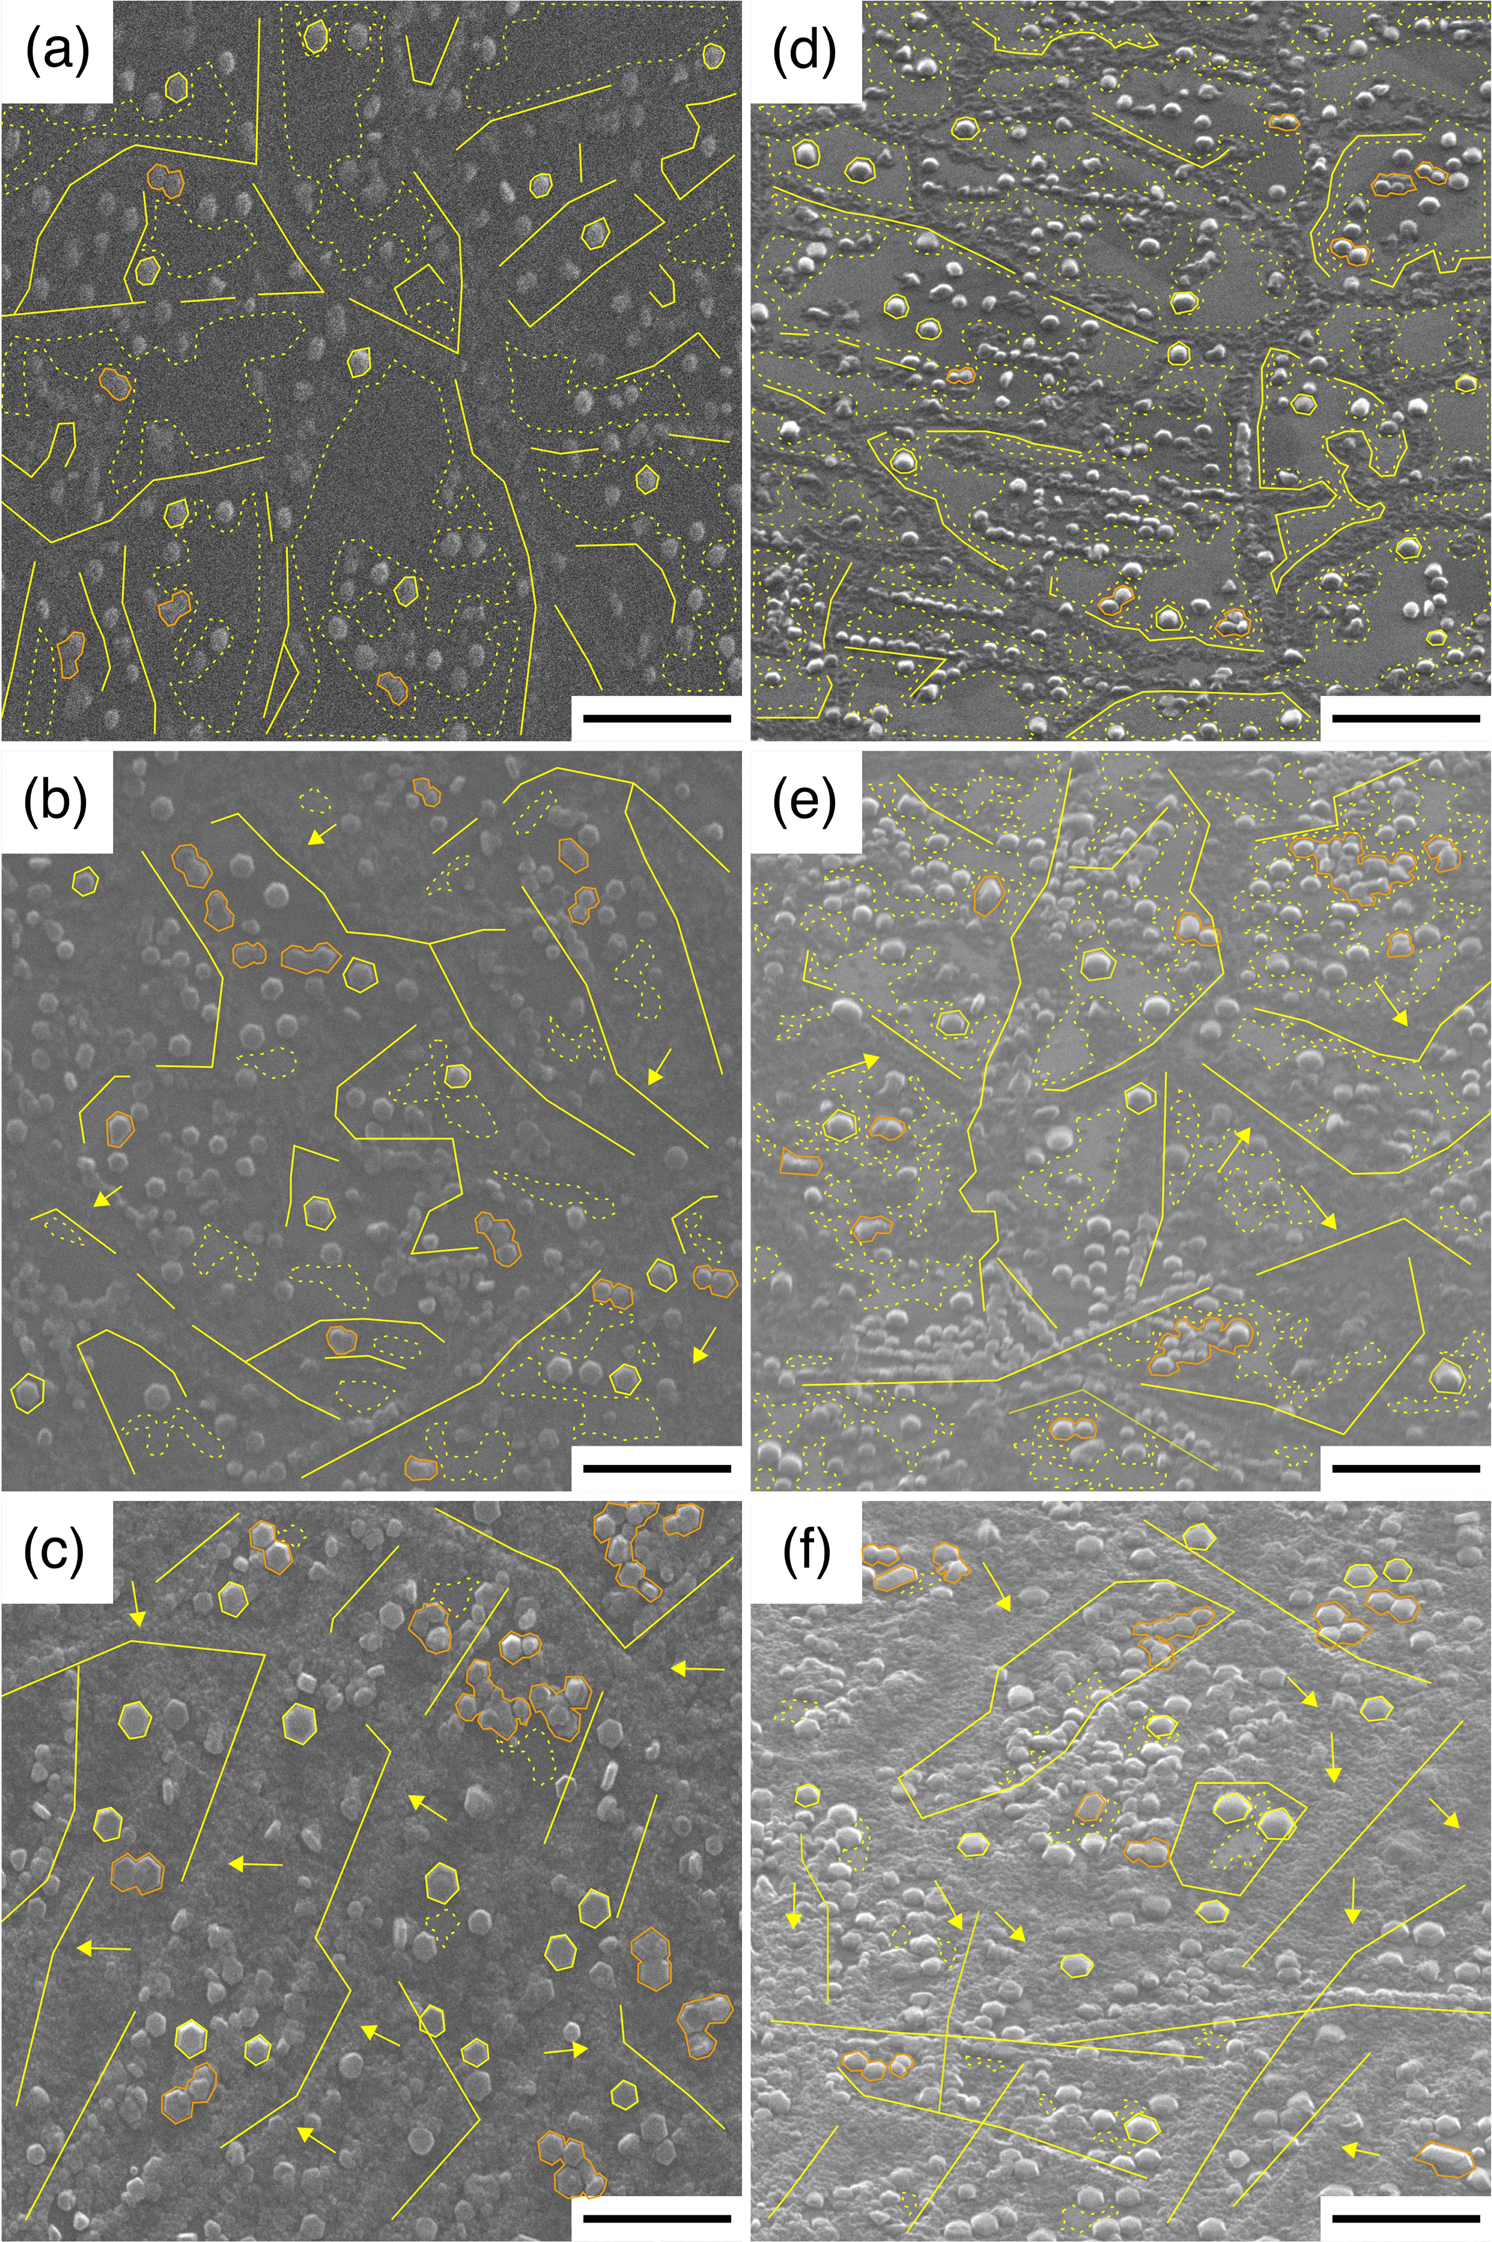
\includegraphics[width=0.95\textwidth]{figures/paper-iv/fig-1.png}
%    \caption[SEM images of AlN on graphene formed via different MEE cycles]{SEM images of AlN on graphene formed via different MEE cycles. (\textbf{a},\textbf{d}), (\textbf{b},\textbf{e}) and (\textbf{c},\textbf{f}) are (top-, bird’s eye-view) SEM images of samples A1, A2 and A3, respectively. Scale bars are 1 {\textmu}m. Features marked with yellow lines, yellow (orange) contours and yellow dashed outlines are high-density AlN nanostructures grown along line defects of graphene, individual (coalesced) AlN islands and areas of exposed graphene, respectively. Yellow arrows in samples A2 and A3 show the lateral growth of AlN nanostructures that initially nucleate at the line defects of graphene in sample A1 (adapted with permission from ref. \citenum{liudimulyo2020853} \copyright \ Liudi Mulyo \textit{et al}, 2020.}
%    \label{fig:figures/paper-iv/fig-1}
%\end{figure}

%\section{Section 1 in chapter 1}
%\lipsum[2]

%\begin{equation}
%    EQE = \frac{q \times P_{opt}}{I \times h\nu}
%\end{equation}

%\lipsum[3-4]

%\subsection{Subsection 1.1 of section 1 in chapter 1}
%\lipsum[5-7]

%\subsection{Subsection 1.2 of section 1 in chapter 1}
%\lipsum[8-10]

%\clearpage\phantomsection % to fix wrong hyperref to this section
%\section[Long section title displayed in the table of content]{Short section title in the chapter}
%\sectionmark{Even shorter title on the header}
%\lipsum[11-20]

%\subsection{Subsection 1.2 of section 2 in chapter 1}
%\lipsum[13-14]

%=======================================================================
%%% References 

% \clearpage
\phantomsection
\specialsection % put an indent, see preamble
\headerspecialsection

{\hypersetup{urlcolor=ntnu,linkcolor=sophia} % set clickable URL title color to black, not ntnu like in the main document

\bibliographystyle{unsrtnat-mod}  % NATBIB ref style
\bibliography{references}
}

\chapter[Introduction]{Introduction}
\markboth{Chap. 1\ \ \enspace Introduction}{Chap 1. Introduction}

\regularsection
\headerregularsection

\updatemylof % to be used with "list of figure divider per chapter" (see PREAMBLE)

\begin{sloppypar} % to suppress overfull box

%Lorem \index{Lorem} ipsum dolor sit amet, consectetuer adipiscing elit \cite{LIUDIMULYO201767}. Ut purus \index{purus} elit,vestibulum ut, placerat ac, adipiscing vitae, felis \citenum{LIUDIMULYO201767}. Curabitur dictum \index{dictum} gravidamauris. Nam arcu libero, nonummy eget, consectetuer id, vulputate a, magna. Donec vehicula augue eu neque \cite{liudimulyo_2018}. Pellentesque habitant morbi tristique senectuset netus et malesuada fames ac turpis egestas \index{egestas}\citenum{liudimulyo_2018}. Mauris ut leo. Cras viverra metusrhoncus sem \cite{2019liudimulyo}. Nulla et lectus vestibulum urna fringilla ultrices. Phasellus eutellus sit amet tortor gravida placerat \citenum{2019liudimulyo}. Integer sapien est, iaculis in, pretium quis,viverra ac, nunc. Praesent eget sem vel leo ultrices bibendum \cite{liudimulyo2020853}. Aenean faucibus. Morbi dolor nulla, malesuada eu, pulvinar at (\ref{fig:figures/paper-iv/fig-1}), mollis ac, nulla. Curabitur auctorsemper nulla \citenum{liudimulyo2020853}. Donec varius orci eget risus. Duis nibh mi, congue eu, accumsaneleifend, sagittis quis, diam. Duis eget orci sit amet orci dignissim rutrum \cite{LIUDIMULYO201767,liudimulyo_2018,2019liudimulyo,liudimulyo2020853,liudimulyo_unpublished1,liudimulyo_unpublished2}.


A vehicle (from Latin: vehiculum \cite{vehicleDef}) is a machine that transports people or cargo. Vehicles include wagons, bicycles, motor vehicles (motorcycles, cars, trucks, buses), railed vehicles (trains, trams), watercraft (ships, boats), amphibious vehicles (screw-propelled vehicle, hovercraft), aircraft (airplanes, helicopters, aerostat) and spacecraft \cite{wikipediaVehicle}. Land vehicles are classified broadly by what is used to apply steering and drive forces against the ground: wheeled, tracked, railed or skied. ISO 3833-1977 is the standard, also internationally used in legislation, for road vehicles types, terms and definitions. Vehicle detection and vehicle type recognition is a practical application of machine learning concepts and is directly applicable for various operations in a traffic surveillance system contributing to an intelligent traffic surveillance system. We will introduce the processing of automatic vehicle detection and recognition using static image datasets. Further using the same technique, we shall improvise vehicle detection by using live CCTV surveillance. The surveillance system includes detection of moving vehicles and recognizing them, counting number of vehicles and verification of their permit with the organization \cite{SriashikaAddala2020}.

Intelligent vehicle detection and counting are becoming increasingly important in the field of highway management. However, due to the different sizes of vehicles, their detection remains a challenge that directly affects the accuracy of vehicle counts. To address this issue, this paper proposes a vision-based vehicle detection and counting system. In the proposed vehicle detection and counting system, the highway road surface in the image is first extracted and divided into a remote area; the method is crucial for improving vehicle detection. Then, the vehicle trajectories are obtained by the ORB algorithm. Finally, the above two areas are placed into the YOLOv5 network to detect the type and location of the vehicle. Several highway surveillance videos based on different scenes are used to verify the proposed methods. The experimental results verify that using the proposed segmentation method can provide higher detection accuracy, especially for the detection of small vehicle object \cite{SongH2019}. 

Vehicle detection and statistics in highway monitoring video scenes are of considerable significance to intelligent traffic management and control of the highway. With the popular installation of traffic surveillance cameras, a vast database of traffic video footage has been obtained for analysis. Generally, at a high viewing angle, a more-distant road surface can be considered. The object size of the vehicle changes greatly at this viewing angle, and the detection accuracy of a small object far away from the road is low. In the face of complex camera scenes, it is essential to effectively solve the above problems and further apply them \cite{SongH2019}. 

A CCTV camera is a very essential part of an intelligent traffic surveillance framework. It is simply the automated process of monitoring the traffic in a particular area and detecting vehicles for further action, as shown in the diagram. The captured images can provide valuable clues to the cops and other public essential tracking services, such as vehicle’s license plate number, time and motion of vehicle, details associated with the driver, etc.. which all may lead to evidence of some crime or any unforeseen or unfortunate incidents. Earlier people used to process images manually. In fact, this system is still going on in India, whereas countries like the USA also have implemented automated machines- CCTVs that function 24x7 and take immediate action via signaling too. Manual work has always been proven slower and less efficient due to human errors and many other factors that affect living beings. Keeping these points in mind and moving with the advancement of technologies, many innovative thinkers have developed certain intelligent traffic control systems using various techniques. This research is based upon the combination of two prior-made researches by scholars whose works have been published \cite{Baran2016}.

\end{sloppypar}

%\begin{figure} % \begin{figure} will let LaTeX decide the best figure placement for you ; \begin{figure}[H] for forcing the figure placement here ; in the bottom, \begin{figure}[!b] ; top of the page, \begin{figure}[!t]
%    \centering
%    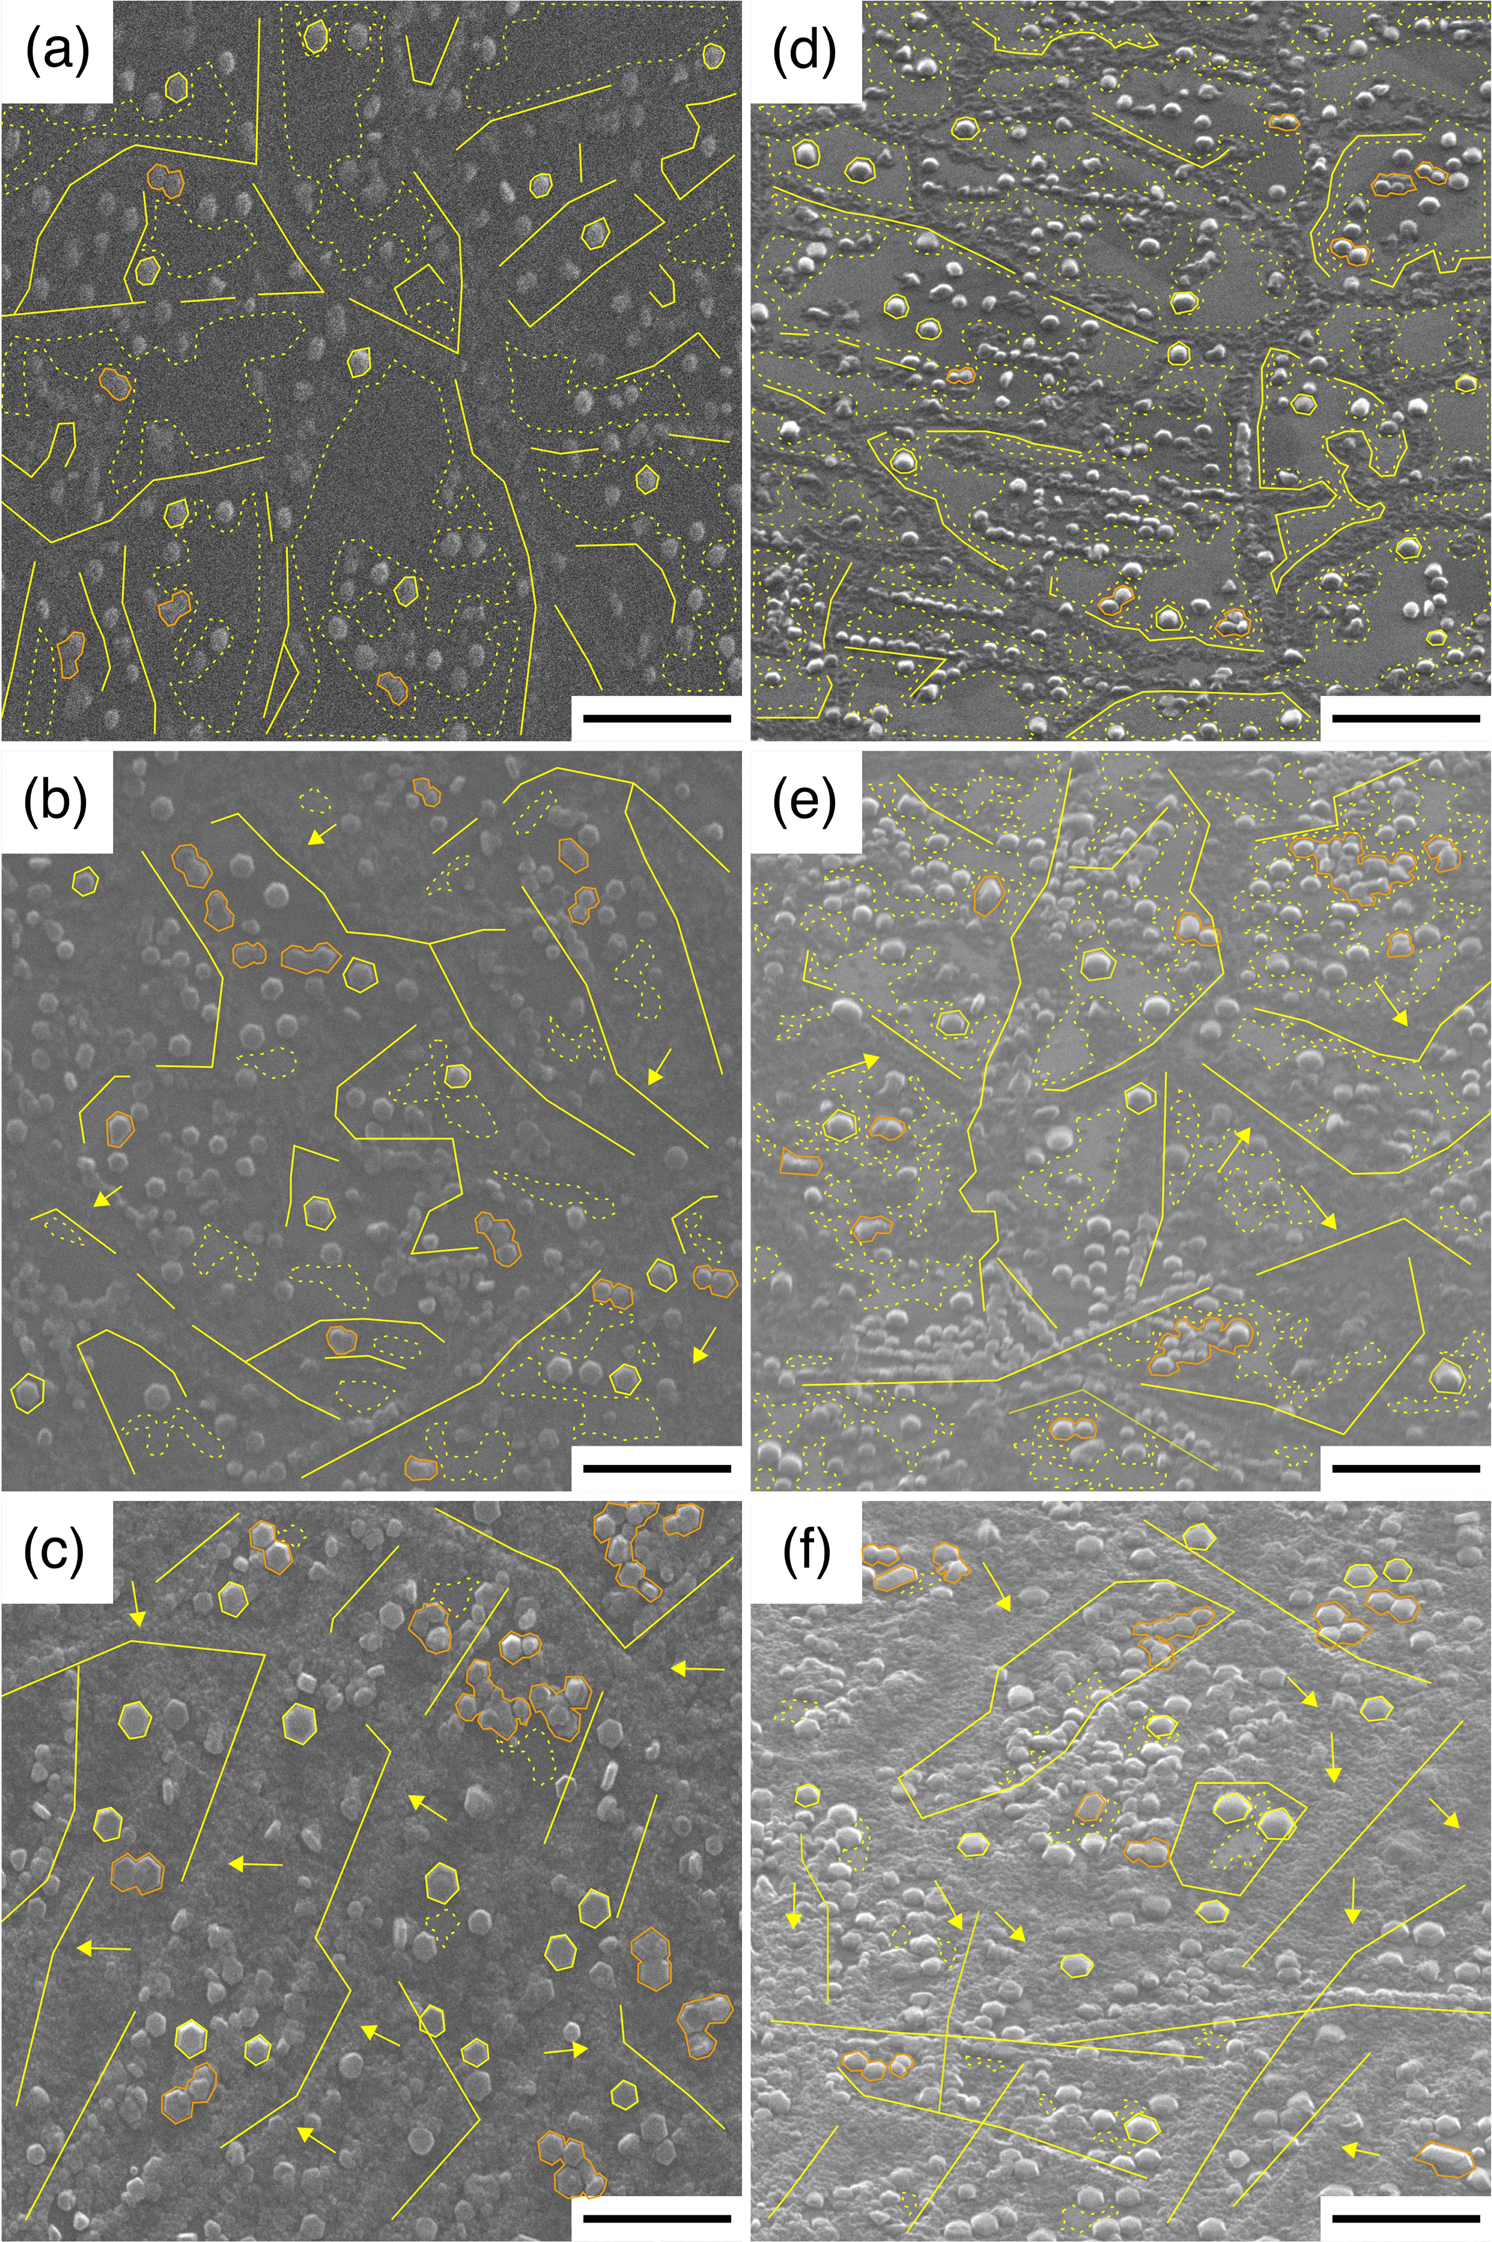
\includegraphics[width=0.95\textwidth]{figures/paper-iv/fig-1.png}
%    \caption[SEM images of AlN on graphene formed via different MEE cycles]{SEM images of AlN on graphene formed via different MEE cycles. (\textbf{a},\textbf{d}), (\textbf{b},\textbf{e}) and (\textbf{c},\textbf{f}) are (top-, bird’s eye-view) SEM images of samples A1, A2 and A3, respectively. Scale bars are 1 {\textmu}m. Features marked with yellow lines, yellow (orange) contours and yellow dashed outlines are high-density AlN nanostructures grown along line defects of graphene, individual (coalesced) AlN islands and areas of exposed graphene, respectively. Yellow arrows in samples A2 and A3 show the lateral growth of AlN nanostructures that initially nucleate at the line defects of graphene in sample A1 (adapted with permission from ref. \citenum{liudimulyo2020853} \copyright \ Liudi Mulyo \textit{et al}, 2020.}
%    \label{fig:figures/paper-iv/fig-1}
%\end{figure}

%\section{Section 1 in chapter 1}
%\lipsum[2]

%\begin{equation}
%    EQE = \frac{q \times P_{opt}}{I \times h\nu}
%\end{equation}

%\lipsum[3-4]

%\subsection{Subsection 1.1 of section 1 in chapter 1}
%\lipsum[5-7]

%\subsection{Subsection 1.2 of section 1 in chapter 1}
%\lipsum[8-10]

%\clearpage\phantomsection % to fix wrong hyperref to this section
%\section[Long section title displayed in the table of content]{Short section title in the chapter}
%\sectionmark{Even shorter title on the header}
%\lipsum[11-20]

%\subsection{Subsection 1.2 of section 2 in chapter 1}
%\lipsum[13-14]

%=======================================================================
%%% References 

% \clearpage
\phantomsection
\specialsection % put an indent, see preamble
\headerspecialsection

{\hypersetup{urlcolor=ntnu,linkcolor=sophia} % set clickable URL title color to black, not ntnu like in the main document

\bibliographystyle{unsrtnat-mod}  % NATBIB ref style
\bibliography{references}
}

\chapter[Related Works]{Related Works}
\markboth{Chap. 1\ \ \enspace Introduction}{Chap 1. Introduction}

\regularsection
\headerregularsection

\updatemylof % to be used with "list of figure divider per chapter" (see PREAMBLE)

\begin{sloppypar} % to suppress overfull box

%Lorem \index{Lorem} ipsum dolor sit amet, consectetuer adipiscing elit \cite{LIUDIMULYO201767}. Ut purus \index{purus} elit,vestibulum ut, placerat ac, adipiscing vitae, felis \citenum{LIUDIMULYO201767}. Curabitur dictum \index{dictum} gravidamauris. Nam arcu libero, nonummy eget, consectetuer id, vulputate a, magna. Donec vehicula augue eu neque \cite{liudimulyo_2018}. Pellentesque habitant morbi tristique senectuset netus et malesuada fames ac turpis egestas \index{egestas}\citenum{liudimulyo_2018}. Mauris ut leo. Cras viverra metusrhoncus sem \cite{2019liudimulyo}. Nulla et lectus vestibulum urna fringilla ultrices. Phasellus eutellus sit amet tortor gravida placerat \citenum{2019liudimulyo}. Integer sapien est, iaculis in, pretium quis,viverra ac, nunc. Praesent eget sem vel leo ultrices bibendum \cite{liudimulyo2020853}. Aenean faucibus. Morbi dolor nulla, malesuada eu, pulvinar at (\ref{fig:figures/paper-iv/fig-1}), mollis ac, nulla. Curabitur auctorsemper nulla \citenum{liudimulyo2020853}. Donec varius orci eget risus. Duis nibh mi, congue eu, accumsaneleifend, sagittis quis, diam. Duis eget orci sit amet orci dignissim rutrum \cite{LIUDIMULYO201767,liudimulyo_2018,2019liudimulyo,liudimulyo2020853,liudimulyo_unpublished1,liudimulyo_unpublished2}.


At present, vision-based vehicle object detection is divided into traditional machine vision methods and complex deep learning methods. Traditional machine vision methods use the motion of a vehicle to separate it from a fixed background image. This method can be divided into three categories: the method of using background subtraction, the method of using continuous video frame difference, and the method of using optical flow. Using the video frame difference method, the variance is calculated according to the pixel values of two or three consecutive video frames. Moreover, the moving foreground region is separated by the threshold. By using this method and suppressing noise, the stopping of the vehicle can also be detected. When the background image in the video is fixed, the background information is used to establish the background model. Then, each frame image is compared with the background model, and the moving object can also be segmented. The method of using optical flow can detect the motion region in the video. The generated optical flow field represents each pixel’s direction of motion and pixel speed. Vehicle detection methods using vehicle features, such as the Scale Invariant Feature Transform (SIFT) and Speeded Up Robust Features (SURF) methods, have been widely used. For example, 3D models have been used to complete vehicle detection and classification tasks. Using the correlation curves of 3D ridges on the outer surface of the vehicle, the vehicles are divided into three categories: cars, SUVs, and minibuses.
The use of deep convolutional networks (CNNs) has achieved amazing success in the field of vehicle object detection. CNNs have a strong ability to learn image features and can perform multiple related tasks, such as classification and bounding box regression. The detection method can be generally divided into two categories. The two-stage method generates a candidate box of the object via various algorithms and then classifies the object by a convolutional neural network. The one-stage method does not generate a candidate box but directly converts the positioning problem of the object bounding box into a regression problem for processing. In the two-stage method, Region-CNN (R-CNN) uses selective region search in the image. The image input to the convolutional network must be fixed-size, and the deeper structure of the network requires a long training time and consumes a large amount of storage memory. Drawing on the idea of spatial pyramid matching, SPP NET  allows the network to input images of various sizes and to have fixed outputs. R-FCN, FPN, and Mask RCNN have improved the feature extraction methods, feature selection, and classification capabilities of convolutional networks in different ways. Among the one-stage methods, the most important are the Single Shot Multibox Detector (SSD) and You Only Look Once (YOLO)  frameworks. The MutiBox, Region Proposal Network (RPN) and multi-scale representation methods are used in SSD, which uses a default set of anchor boxes with different aspect ratios to more accurately position the object. Unlike SSD, the YOLO network divides the image into a fixed number of grids. Each grid is responsible for predicting objects whose centre points are within the grid. YOLOv2 added the BN (Batch Normalization) layer, which makes the network normalize the input of each layer and accelerate the network convergence speed. YOLOv2 uses a multi-scale training method to randomly select a new image size for every ten batches. Our vehicle object detection uses the YOLOv3  network. Based on YOLOv2, YOLOv3 uses logistic regression for the object category. The category loss method is two-class cross-entropy loss, which can handle multiple label problems for the same object. Moreover, logistic regression is used to regress the box confidence to determine if the IOU of the a priori box and the actual box is greater than 0.5. If more than one priority box satisfies the condition, only the largest prior box of the IOU is taken. In the final object prediction, YOLOv3 uses three different scales to predict the object in the image.
The traditional machine vision method has a faster speed when detecting the vehicle but does not produce a good result when the image changes in brightness, there is periodic motion in the background, and where there are slow moving vehicles or complex scenes. Advanced CNN has achieved good results in object detection; however, CNN is sensitive to scale changes in object detection. The one stage method uses grids to predict objects, and the grid’s spatial constraints make it impossible to have higher precision with the two-stage approach, especially for small objects. The two stage method uses region of interest pooling to segment candidate regions into blocks according to given parameters, and if the candidate region is smaller than the size of the given parameters, the candidate region is padded to the size of the given parameters. In this way, the characteristic structure of a small object is destroyed and its detection accuracy is low. The existing methods do not distinguish if large and small objects belong to the same category. The same method is used to deal with the same type of object, which will also lead to inaccurate detection. The use of image pyramids or multi-scale input images can solve the above problems, although the calculation requirements are large.


Detection of specific objects in images is difficult, due to the nature of objects in images that are often of different sizes, different orientations, and overlapping objects that causes occlusion of the object of interest to be detected. These problems require a detection algorithm that has several properties, such as translation invariance(invariant to different locations of object of interest in the image), rotation invariance (invariant to the rotation of the object in the image), and scale invariance (invariant to the size of the objects in the image). A common approach is to use machine learning methods that learn a representation directly from the available data to train a model. Popular Methods use low level features such as SIFT [12], HOG [3], and Haar [17] combining them with a machine learning method to classify the objects. This approach is known as the “Feature +Classifier'' approach.

\section{Vehicle detection research in Europe}
Vision-based vehicle detection methods in Europe have achieved abundant results. In, between the “Hofolding” and “Weyern” sections of the A8 motorway in Munich, Germany, the Multivariate Alteration Detection (MAD) method was used to detect the change of two images with a short time lag. The moving vehicles are highlighted in a change image, which is used to estimate the vehicle density of the road. Using the motorways A95 and A96 near Munich, the A4 near Dresden, and the “Mittlere Ring” in Munich as the test environments, the Canny edge algorithm is applied to the road image, and the histogram of the edge steepness is calculated. Then, using the k-means algorithm, the edge steepness statistics are divided into three parts, and a closed vehicle model is detected based on the steepness. A contrast-based approach was used to create a colour model to identify and remove vehicle shadow areas, which eliminates interference caused by movement in the scene. After eliminating the shadow area, the vehicle detection performance can be significantly improved. The experiment was conducted on Italian and French highways. The HOG and Haar-like features were compared in, and the two features were merged to construct a detector for vehicle detection that was tested on French vehicle images. However, when the above method is used for vehicle detection, the type of vehicle cannot be detected. Additionally, when the illumination is insufficient, it is difficult to extract the edge of the vehicle or detect the moving car, which causes problems in low vehicle detection accuracy and affects the detection results for further use. Pictures of aerial view angles were used by but cannot clearly capture the characteristics of each car and produce false vehicle detections.
Nonetheless, with the development of deep learning technology, vehicle detection based on CNN has been successfully applied in Europe. In Fast R-CNN was used for vehicle detection in traffic scenes in the city of Karlsruhe, Germany. Fast R-CNN uses a selective search strategy to find all candidate frames, which is notably time-consuming, and the vehicle detection speed is slow.
In short, research on vision-based vehicle detection is still progressing, and major challenges are gradually being overcome, which will make a significant contribution to the development of European traffic construction.


\end{sloppypar}

%\begin{figure} % \begin{figure} will let LaTeX decide the best figure placement for you ; \begin{figure}[H] for forcing the figure placement here ; in the bottom, \begin{figure}[!b] ; top of the page, \begin{figure}[!t]
%    \centering
%    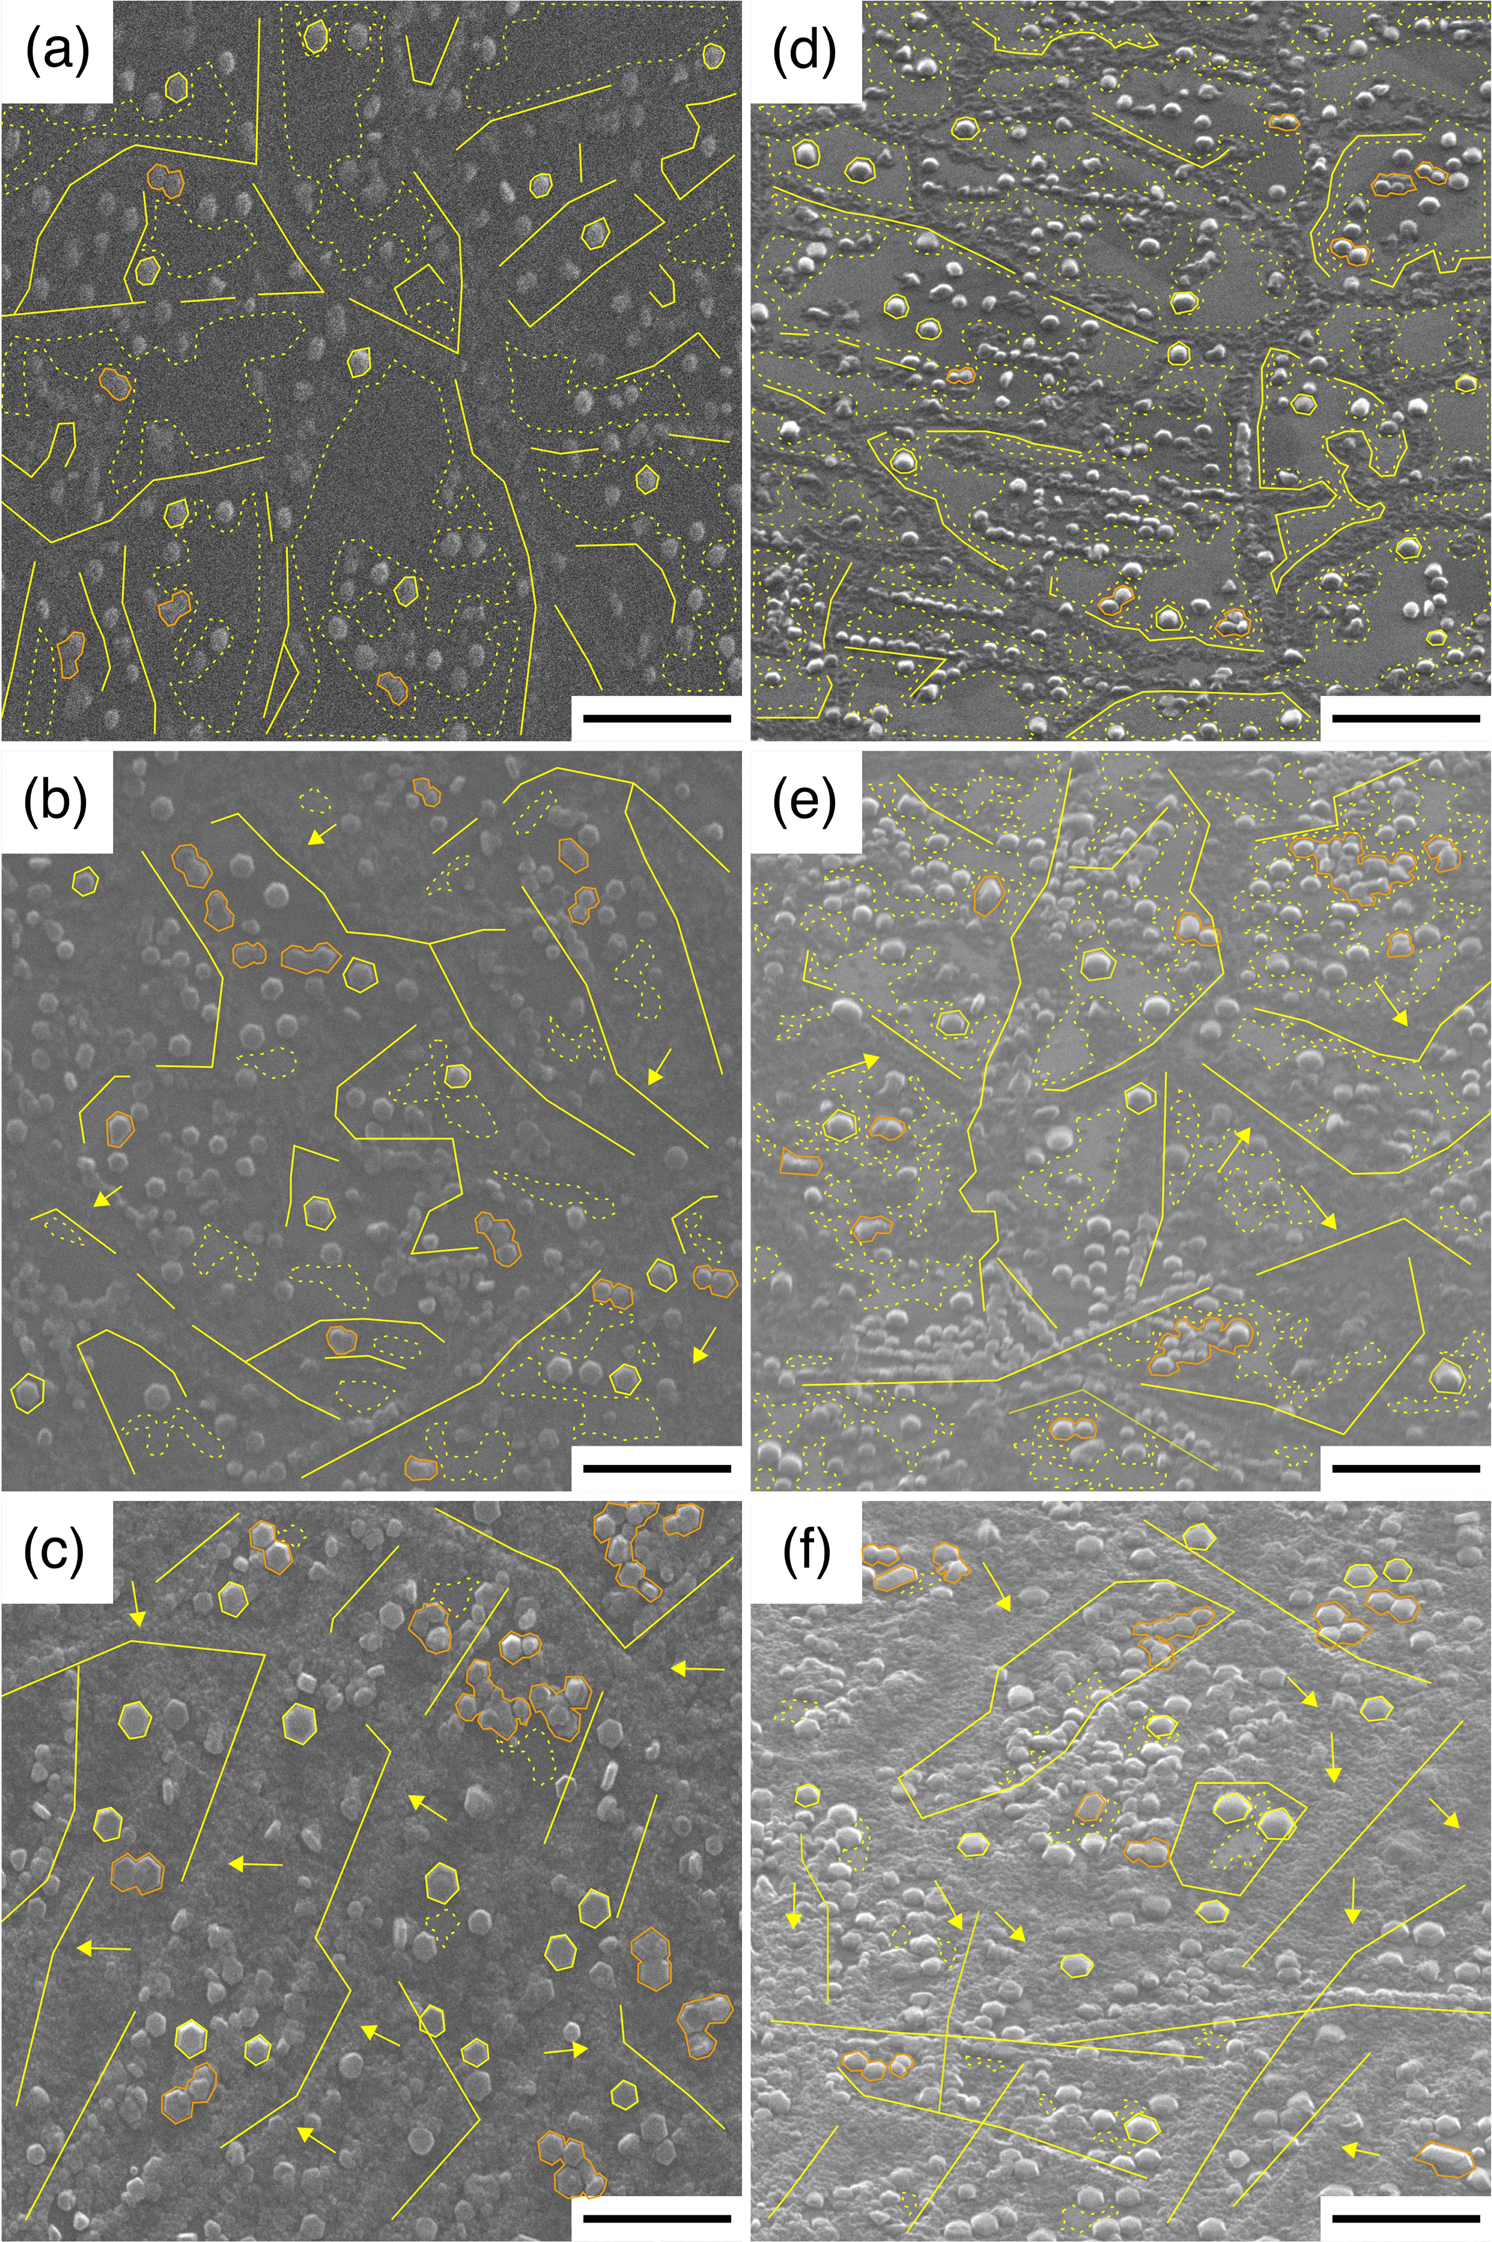
\includegraphics[width=0.95\textwidth]{figures/paper-iv/fig-1.png}
%    \caption[SEM images of AlN on graphene formed via different MEE cycles]{SEM images of AlN on graphene formed via different MEE cycles. (\textbf{a},\textbf{d}), (\textbf{b},\textbf{e}) and (\textbf{c},\textbf{f}) are (top-, bird’s eye-view) SEM images of samples A1, A2 and A3, respectively. Scale bars are 1 {\textmu}m. Features marked with yellow lines, yellow (orange) contours and yellow dashed outlines are high-density AlN nanostructures grown along line defects of graphene, individual (coalesced) AlN islands and areas of exposed graphene, respectively. Yellow arrows in samples A2 and A3 show the lateral growth of AlN nanostructures that initially nucleate at the line defects of graphene in sample A1 (adapted with permission from ref. \citenum{liudimulyo2020853} \copyright \ Liudi Mulyo \textit{et al}, 2020.}
%    \label{fig:figures/paper-iv/fig-1}
%\end{figure}

%\section{Section 1 in chapter 1}
%\lipsum[2]

%\begin{equation}
%    EQE = \frac{q \times P_{opt}}{I \times h\nu}
%\end{equation}

%\lipsum[3-4]

%\subsection{Subsection 1.1 of section 1 in chapter 1}
%\lipsum[5-7]

%\subsection{Subsection 1.2 of section 1 in chapter 1}
%\lipsum[8-10]

%\clearpage\phantomsection % to fix wrong hyperref to this section
%\section[Long section title displayed in the table of content]{Short section title in the chapter}
%\sectionmark{Even shorter title on the header}
%\lipsum[11-20]

%\subsection{Subsection 1.2 of section 2 in chapter 1}
%\lipsum[13-14]

%=======================================================================
%%% References 

% \clearpage
\phantomsection
\specialsection % put an indent, see preamble
\headerspecialsection

{\hypersetup{urlcolor=ntnu,linkcolor=sophia} % set clickable URL title color to black, not ntnu like in the main document

\bibliographystyle{unsrtnat-mod}  % NATBIB ref style
\bibliography{references}
}

\chapter[Object Detection With YOLO]{Object Detection With YOLO}
\markboth{Chap. 1\ \ \enspace Introduction}{Chap 1. Introduction}

\regularsection
\headerregularsection

\updatemylof % to be used with "list of figure divider per chapter" (see PREAMBLE)

\begin{sloppypar} % to suppress overfull box

  %Lorem \index{Lorem} ipsum dolor sit amet, consectetuer adipiscing elit \cite{LIUDIMULYO201767}. Ut purus \index{purus} elit,vestibulum ut, placerat ac, adipiscing vitae, felis \citenum{LIUDIMULYO201767}. Curabitur dictum \index{dictum} gravidamauris. Nam arcu libero, nonummy eget, consectetuer id, vulputate a, magna. Donec vehicula augue eu neque \cite{liudimulyo_2018}. Pellentesque habitant morbi tristique senectuset netus et malesuada fames ac turpis egestas \index{egestas}\citenum{liudimulyo_2018}. Mauris ut leo. Cras viverra metusrhoncus sem \cite{2019liudimulyo}. Nulla et lectus vestibulum urna fringilla ultrices. Phasellus eutellus sit amet tortor gravida placerat \citenum{2019liudimulyo}. Integer sapien est, iaculis in, pretium quis,viverra ac, nunc. Praesent eget sem vel leo ultrices bibendum \cite{liudimulyo2020853}. Aenean faucibus. Morbi dolor nulla, malesuada eu, pulvinar at (\ref{fig:figures/paper-iv/fig-1}), mollis ac, nulla. Curabitur auctorsemper nulla \citenum{liudimulyo2020853}. Donec varius orci eget risus. Duis nibh mi, congue eu, accumsaneleifend, sagittis quis, diam. Duis eget orci sit amet orci dignissim rutrum \cite{LIUDIMULYO201767,liudimulyo_2018,2019liudimulyo,liudimulyo2020853,liudimulyo_unpublished1,liudimulyo_unpublished2}.


  YOLO (You Only Look Once) is a state-of-art algorithm devoted to object detection, as the name
  implies it can predict objects just by looking once to the image in a clever way. YOLO makes the
  prediction by classifying the object and locating it in the image. It uses deep learning and CNN
  techniques to detect objects, and distinguishes itself from its competitors because, as its name
  indicates, it requires to see the image only once, allowing it to be the fastest of all although it
  sacrifices a little accuracy. This speed allows users to easily detect objects in real time in videos
  (up to 30 FPS). In other words, YOLO takes as input value an image and passes through the neural
  network that looks like a CNN and returns a vector of bounding boxes and class prediction. To
  understand  better  how  YOLO  makes  the  prediction  we  will  explain  it  with  an  example  of  an
  image as it can be seen in Figure~\ref{fig:figures/paper/yolo-grid}.

\begin{figure}[H] % \begin{figure} will let LaTeX decide the best figure placement for you ; \begin{figure}[H] for forcing the figure placement here ; in the bottom, \begin{figure}[!b] ; top of the page, \begin{figure}[!t]
  \centering
  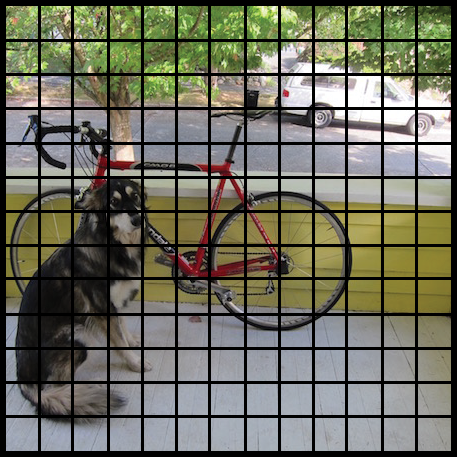
\includegraphics[width=0.60\textwidth]{figures/paper/yolo-grid.png}
  \caption[YOLO divides up the image into a grid of 13 by 13 cells]{YOLO divides up the image into a grid of 13 by 13 cells: Each of these cells is responsible for predicting 5 bounding boxes. A bounding box describes the rectangle that encloses an object.}
  \label{fig:figures/paper/yolo-grid}
\end{figure}


\end{sloppypar}



\section{YOLO in brief}
  To perform de detection YOLO first divides the image into an S x S grid of cells, in Figure~\ref{fig:figures/paper/yolo-grid} we
  can  see  that  the  image  is divided  into  a  13 x  13  grid  of  cells.  In  each of the cells  it  predicts  N
  possible  bounding  boxes  and  calculates  the  level  of  certainty  (probability)  of  each  of  them
  (shown in Figure 13), that is, S x S x N different bounding boxes are calculated in the image, the
  vast majority of them with a very low level of certainty. The score of each BB does not classify
  what type of object is or it does not know what object is fitting the bounding box, it just gives a
  confidence value or a probability value of how good the BB is surrounding an object in each cell.
  In case of Figure~\ref{fig:figures/paper/yolo-grid} for each grid cells 5 bounding boxes are predicted and are graphically shown
  in~\ref{fig:figures/paper/yolo-grid-2} where the higher the probability is the fatter the box is. Each cell makes N bounding
  box predictions and M class probabilities.


  \begin{figure}[H] % \begin{figure} will let LaTeX decide the best figure placement for you ; \begin{figure}[H] for forcing the figure placement here ; in the bottom, \begin{figure}[!b] ; top of the page, \begin{figure}[!t]
  \centering
  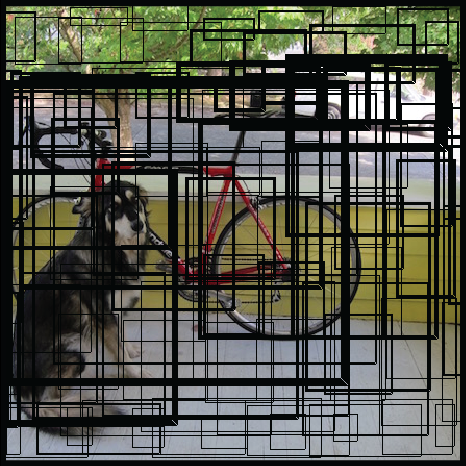
\includegraphics[width=0.60\textwidth]{figures/paper/yolo-grid-2.png}
  \caption[The predicted bounding boxes]{The predicted bounding boxes may look something like this, the higher the confidence score, the fatter the box is drawn}
  \label{fig:figures/paper/yolo-grid-2}
\end{figure}


The bounding box prediction is formed by 5 components: x, y, width, height, confidence score.

\begin{itemize}
\item The (x, y) components are like a mathematical graph coordinates that refer to the centre
of the box, relative to the grid cell location. If the centre of the bounding box does not
fall inside the grid cell this means that the grid cell is not responsible of the object that
has predicted the bounding box. This happens because each object that appears in the
image is related to a single grid cell that is responsible for predicting the object. (x, y)
are normalized between 0 and 1.

\item (Width,  height)  represent  the  dimension  of  the  box  that  contains  an  object,  they  are
also normalized to values from 0 to 1 and they are fundamental to locate the object in
the image.
\item Confidence score  is  a  real value  that  represents  the assurance  the  algorithm  has  that
the box contains an object of any class. The method how the confidence is calculated
will be explained later.

\end{itemize}


\section{The Predictions Vector}
The first step to understanding YOLO is how it encodes its output. The input image is divided into an S x S grid of cells. For each object that is present on the image, one grid cell is said to be “responsible” for predicting it. That is the cell where the center of the object falls into.

Each grid cell predicts B bounding boxes as well as C class probabilities. The bounding box prediction has 5 components: (x, y, w, h, confidence). The (x, y) coordinates represent the center of the box, relative to the grid cell location (remember that, if the center of the box does not fall inside the grid cell, than this cell is not responsible for it). These coordinates are normalized to fall between 0 and 1. The (w, h) box dimensions are also normalized to [0, 1], relative to the image size.


%\section{Section 1 in chapter 1}
%\lipsum[2]

%\begin{equation}
%    EQE = \frac{q \times P_{opt}}{I \times h\nu}
%\end{equation}

%\lipsum[3-4]

%\subsection{Subsection 1.1 of section 1 in chapter 1}
%\lipsum[5-7]

%\subsection{Subsection 1.2 of section 1 in chapter 1}
%\lipsum[8-10]

%\clearpage\phantomsection % to fix wrong hyperref to this section
%\section[Long section title displayed in the table of content]{Short section title in the chapter}
%\sectionmark{Even shorter title on the header}
%\lipsum[11-20]

%\subsection{Subsection 1.2 of section 2 in chapter 1}
%\lipsum[13-14]

%=======================================================================
%%% References

% \clearpage
\phantomsection
\specialsection % put an indent, see preamble
\headerspecialsection

{\hypersetup{urlcolor=ntnu,linkcolor=sophia} % set clickable URL title color to black, not ntnu like in the main document

  \bibliographystyle{unsrtnat-mod}  % NATBIB ref style
  \bibliography{references}
}

 \chapter[Methodology]{Methodology}
\markboth{Chap. 3\ \ \enspace Experimental methods}{Chap 2. Experimental methods}

\regularsection
\headerregularsection

\updatemylof % to be used with "list of figure divider per chapter" (see PREAMBLE)
\updatemylot % to be used with "list of table divider per chapter" (see PREAMBLE)

\begin{sloppypar} % to suppress overfull box

  The Architecture. Our detection network has 24 convolutional layers followed by 2 fully connected layers. Alternating 1 ×1 convolutional layers reduce the features space from preceding layers. We pretrain the convolutional layers on the ImageNet classification task at half the resolution (224 ×224 input image) and then double the resolution for detection.

\end{sloppypar}

\begin{figure}[H] % \begin{figure}[H] for forcing the figure placement here ; in the bottom, \begin{figure}[!b] ; top of the page, \begin{figure}[!t] ; otherwise, \begin{figure} will let LaTeX decide the best figure placement for you
  \centering
  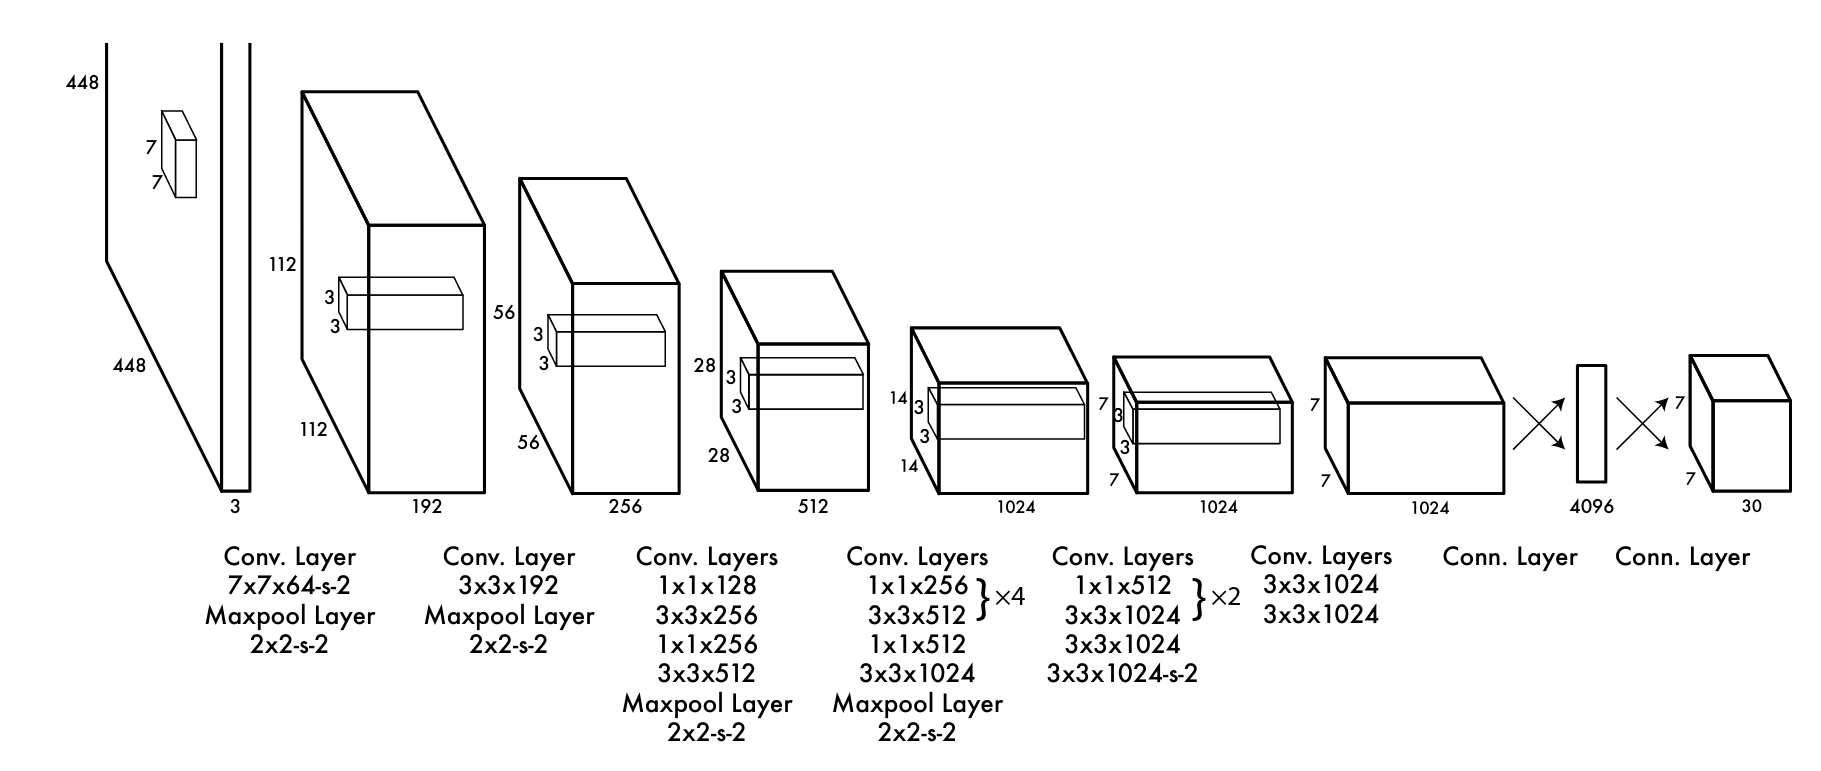
\includegraphics[width=\textwidth]{figures/paper/layers.png}
  \caption[The Architecture]{\textbf{The Architecture}. Our detection network has $24$ convolutional layers followed by $2$ fully connected layers. Alternating $1 \times 1$ convolutional layers reduce the features space from preceding layers. We pretrain the convolutional layers on the ImageNet classification task at half the resolution ($224 \times 224$ input image) and then double the resolution for detection.}
  \label{fig:figures/paper-iv/fig-3}
\end{figure}




\section{The Network}
The network structure looks like a normal CNN, with convolutional and max pooling layers, followed by 2 fully connected layers in the end:


\begin{table}[!h]
  \centering
  \caption[YOLO Network Structure]{YOLO Network Structure}
  \label{tab:yolo-network}
  {\renewcommand{\arraystretch}{1.3}
    \begin{tabular}{c c c}
      \toprule
      Name       &        Filters         & Output Dimension  \\
      \hline
      Conv 1     & 7 x 7 x 64, stride=2   & 224 x 224 x 64    \\
      Max Pool 1 & 2 x 2, stride=2        & 112 x 112 x 64    \\
      Conv 2     & 3 x 3 x 192            & 112 x 112 x 192   \\
      Max Pool 2 & 2 x 2, stride=2        & 56 x 56 x 192     \\
      Conv 3     & 1 x 1 x 128            & 56 x 56 x 128     \\
      Conv 4     & 3 x 3 x 256            & 56 x 56 x 256     \\
      Conv 5     & 1 x 1 x 256            & 56 x 56 x 256     \\
      Conv 6     & 1 x 1 x 512            & 56 x 56 x 512     \\
      Max Pool 3 & 2 x 2, stride=2        & 28 x 28 x 512     \\
      Conv 7     & 1 x 1 x 256            & 28 x 28 x 256     \\
      Conv 8     & 3 x 3 x 512            & 28 x 28 x 512     \\
      Conv 9     & 1 x 1 x 256            & 28 x 28 x 256     \\
      Conv 10    & 3 x 3 x 512            & 28 x 28 x 512     \\
      Conv 11    & 1 x 1 x 256            & 28 x 28 x 256     \\
      Conv 12    & 3 x 3 x 512            & 28 x 28 x 512     \\
      Conv 13    & 1 x 1 x 256            & 28 x 28 x 256     \\
      Conv 14    & 3 x 3 x 512            & 28 x 28 x 512     \\
      Conv 15    & 1 x 1 x 512            & 28 x 28 x 512     \\
      Conv 16    & 3 x 3 x 1024           & 28 x 28 x 1024    \\
      Max Pool 4 & 2 x 2, stride=2        & 14 x 14 x 1024    \\
      Conv 17    & 1 x 1 x 512            & 14 x 14 x 512     \\
      Conv 18    & 3 x 3 x 1024           & 14 x 14 x 1024    \\
      Conv 19    & 1 x 1 x 512            & 14 x 14 x 512     \\
      Conv 20    & 3 x 3 x 1024           & 14 x 14 x 1024    \\
      Conv 21    & 3 x 3 x 1024           & 14 x 14 x 1024    \\
      Conv 22    & 3 x 3 x 1024, stride=2 & 7 x 7 x 1024      \\
      Conv 23    & 3 x 3 x 1024           & 7 x 7 x 1024      \\
      Conv 24    & 3 x 3 x 1024           & 7 x 7 x 1024      \\
      FC 1       & -                      & 4096              \\
      FC 2       & -                      & 7 x 7 x 30 (1470) \\
\bottomrule
    \end{tabular}
  }
\end{table}

Note that the architecture was crafted for use in the Pascal VOC dataset, where the authors used $S=7$, $B=2$ and $C=20$. This explains why the final feature maps are $7 \times 7$, and also explains the size of the output $(7x7x(2 \times 5+20))$. Use of this network with a different grid size or different number of classes might require tuning of the layer dimensions. The authors mention that there is a fast version of YOLO, with fewer convolutional layers. The table~\ref{tab:yolo-network}, however, display the full version. The sequences of 1x1 reduction layers and 3x3 convolutional layers were inspired by the GoogLeNet (Inception) model. The final layer uses a linear activation function. All other layers use a leaky RELU $(\phi(x) = x, if x>0; 0.1x \ otherwise)$.

\section{The Loss Function}
The loss function start like this:
\begin{equation}
  \lambda_{coord} \sum_{i=0}^{S^2}\sum_{j=0}^B \mathbbm{1}_{ij}^{obj}[(x_i-\hat{x}_i)^2 + (y_i-\hat{y}_i)^2 ]
\label{yolo-loss-func}
\end{equation}


This equation computes the loss related to the predicted bounding box position $(x,y)$. Don’t worry about $\lambda$ for now, just consider it a given constant. The function computes a sum over each bounding box predictor $(j = 0..B)$ of each grid cell $(i = 0 .. S^2)$. $\mathbbm{1} obj$ is defined as follows:

\begin{itemize}
  \item 1, If an object is present in grid cell i and the jth bounding box predictor is “responsible” for that prediction
  \item 0, otherwise
\end{itemize}

But how do we know which predictor is responsible for the object? Quoting the original paper:
\begin{quote}
YOLO predicts multiple bounding boxes per grid cell. At training time we only want one bounding box predictor to be responsible for each object. We assign one predictor to be “responsible” for predicting an object based on which prediction has the highest current IOU with the ground truth.
\end{quote}

The other terms in the equation should be easy to understand: $(x, y)$ are the predicted bounding box position and $(\hat{x}, \hat{y})$ hat are the actual position from the training data.

Let’s move on to the second part:
\begin{equation}
  \lambda_{coord} \sum_{i=0}^{S^2}\sum_{j=0}^B \mathbbm{1}_{ij}^{obj}[(\sqrt{w_i}-\sqrt{\hat{w}_i})^2 +(\sqrt{h_i}-\sqrt{\hat{h}_i})^2 ]
\label{yolo-loss-func-2}
\end{equation}


This is the loss related to the predicted box width / height. The equation looks similar to the first one, except for the square root. Quoting the paper again:

\begin{quote}
Our error metric should reflect that small deviations in large boxes matter less than in small boxes. To partially address this we predict the square root of the bounding box width and height instead of the width and height directly.
  \end{quote}

    

Moving on to the third part:
\begin{equation}
  \sum_{i=0}^{S^2}\sum_{j=0}^B \mathbbm{1}_{ij}^{obj}(C_i - \hat{C}_i)^2 + \lambda_{noobj}\sum_{i=0}^{S^2}\sum_{j=0}^B \mathbbm{1}_{ij}^{noobj}(C_i - \hat{C}_i)^2
\label{yolo-loss-func-3}
\end{equation}


Here we compute the loss associated with the confidence score for each bounding box predictor. $C$ is the confidence score and $\hat{C}$ is the intersection over union of the predicted bounding box with the ground truth. $\mathbbm{1} obj$ is equal to one when there is an object in the cell, and 0 otherwise. $\mathbbm{1} noobj$  is the opposite.

The $\lambda $ parameters that appear here and also in the first part are used to differently weight parts of the loss functions. This is necessary to increase model stability. The highest penalty is for coordinate predictions $(\lambda coord = 5)$ and the lowest for confidence predictions when no object is present $(\lambda noobj = 0.5)$.

The last part of the loss function is the classification loss:
\begin{equation}
  \sum_{i=0}^{S^2} \mathbbm{1}_{i}^{obj}\sum_{c \in classes}(p_i(c) - \hat{p}_i(c))^2
\label{yolo-loss-func-4}
\end{equation}

It looks similar to a normal sum-squared error for classification, except for the $\mathbbm{1} obj$ term. This term is used because so we don’t penalize classification error when no object is present on the cell (hence the conditional class probability discussed earlier).

Note that the loss function only penalizes classification error if an object is present in that grid cell (hence the con-ditional class probability discussed earlier). It also only pe-nalizes bounding box coordinate error if that predictor is “responsible” for the ground truth box (i.e. has the highest IOU of any predictor in that grid cell). \cite{redmon2016look}


%=======================================================================
%%% References

% \clearpage
\phantomsection
\specialsection % put an indent, see preamble
\headerspecialsection

{\hypersetup{urlcolor=ntnu,linkcolor=sophia} % set clickable URL title color to black, not ntnu like in the main document

  \bibliographystyle{unsrtnat-mod}  % NATBIB ref style
  \bibliography{references}
}

 \chapter[Dataset]{Dataset}
\markboth{Chap. 3\ \ \enspace Experimental methods}{Chap 2. Experimental methods}

\regularsection
\headerregularsection

\updatemylof % to be used with "list of figure divider per chapter" (see PREAMBLE)
\updatemylot % to be used with "list of table divider per chapter" (see PREAMBLE)

\begin{sloppypar} % to suppress overfull box

  Our new benchmark has 100000 cropped images after discarding some of the images only containing background. Of these, 10000 contain 30000 traffic signs in total. Although our source images cover much of Bangladesh and India, an imbalance still exists between different classes of traffic sign in our benchmark. This is unavoidable: classes such as signs. It can be from different viewpoints, have different ground sampling distances (gsd), different image sizes, aspect ratios, color, etc. Vehicles in different data may be significantly different in size and appearance. Figure~\ref{fig:figures/paper/dataset/collage.jpg} shows different images from four different datasets. It is obvious how different the VOC data is from any of the elevated data, while the VEDAI and AFVID data are somewhat similar, and the AF Build-ing Camera data is more similar to the aerial and satellite data. A more detailed look at the aerial datasets is available in TableNumber of classesIn the configuration file that defines the YOLO net model there is a 'classes' definition that is used to define the number of classes. To change the number of classes used, more than just the classes setting will need to be changed; the number of filters in the last convolutional layer must be altered to reflect the changed number of classes. The number of filters is set by $num(classes + coords + 1)$, where num isnumber of anchor boxes, and coords is four corresponding to the four coordinates used to define a bounding box.

\end{sloppypar}

\begin{figure}[H] % \begin{figure}[H] for forcing the figure placement here ; in the bottom, \begin{figure}[!b] ; top of the page, \begin{figure}[!t] ; otherwise, \begin{figure} will let LaTeX decide the best figure placement for you
  \centering
  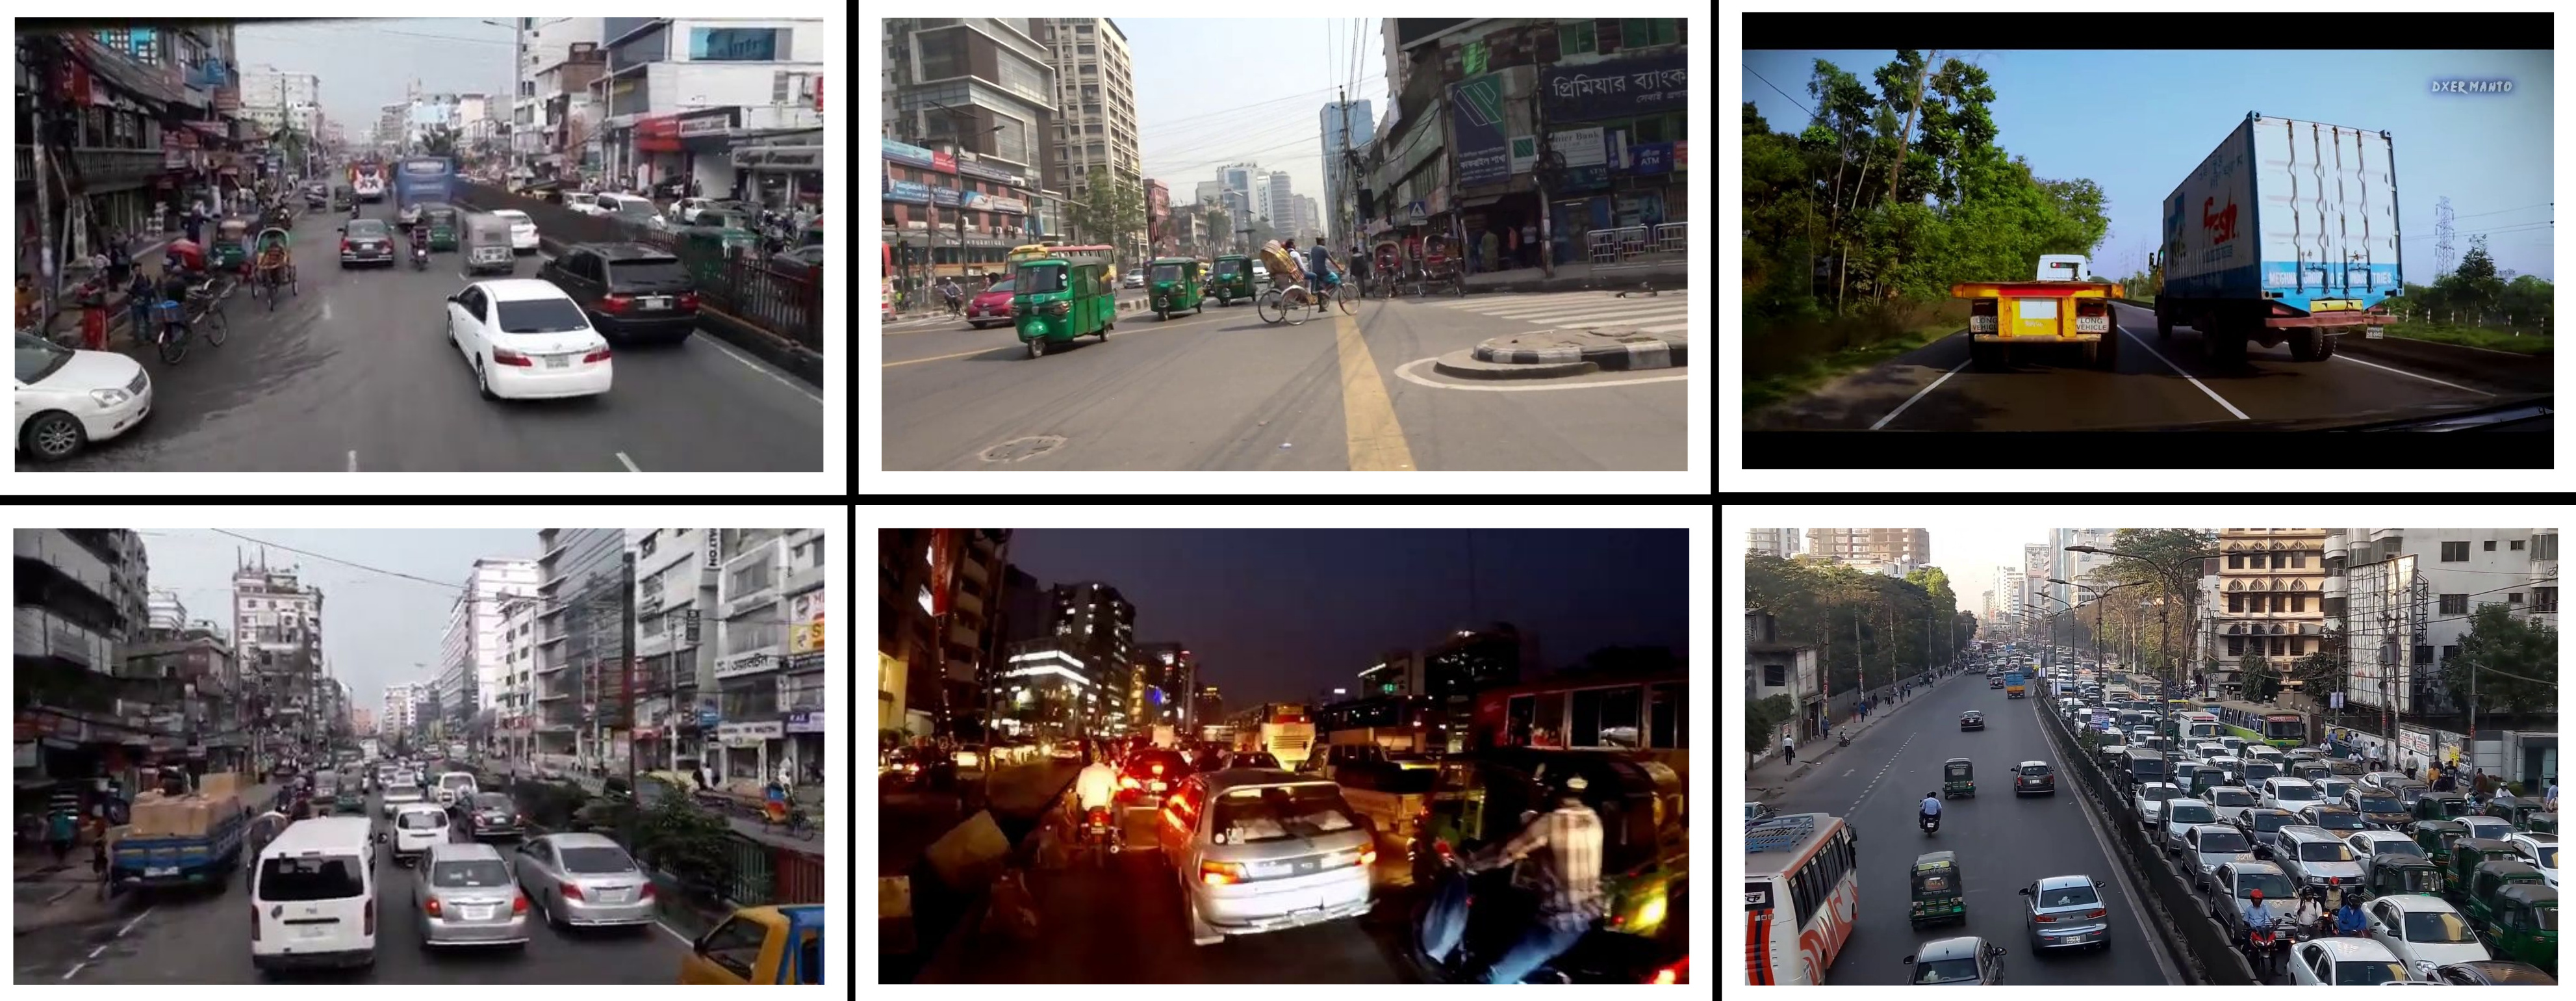
\includegraphics[width=\textwidth]{figures/paper/dataset-collage.jpg}
  \caption[Dataset Collage]{\textbf{Dataset Collage}. Some sample data from Dhaka AI dataset.}
  \label{fig:figures/paper/dataset-collage.jpg}
\end{figure}



\section{COCO Dataset Details}
\begin{itemize}
  \item \textbf{Images per class} ≥ 1500 images per class recommended
  \item \textbf{Instances per class} ≥ 10000 instances (labeled objects) per class recommended
  \item \textbf{Image variety} Must be representative of deployed environment. For real-world use cases we recommend images from different times of day, different seasons, different weather, different lighting, different angles, different sources (scraped online, collected locally, different cameras) etc.
 \item \textbf{Label consistency} All instances of all classes in all images must be labelled. Partial labelling will not work.
 \item \textbf{Label accuracy} Labels must closely enclose each object. No space should exist between an object and it's bounding box. No objects should be missing a label.
 \item \textbf{Background images} Background images are images with no objects that are added to a dataset to reduce False Positives (FP). We recommend about 0-10\% background images to help reduce FPs (COCO has 1000 background images for reference, 1\% of the total). No labels are required for background images.
\end{itemize}


\section{Dhaka AI Dataset}
We have used  a mixed dataset from Indian Driving Dataset and Dhaka AI Traffic Detection Challenge Dataset. 
\begin{figure}[H] % \begin{figure}[H] for forcing the figure placement here ; in the bottom, \begin{figure}[!b] ; top of the page, \begin{figure}[!t] ; otherwise, \begin{figure} will let LaTeX decide the best figure placement for you
  \centering
  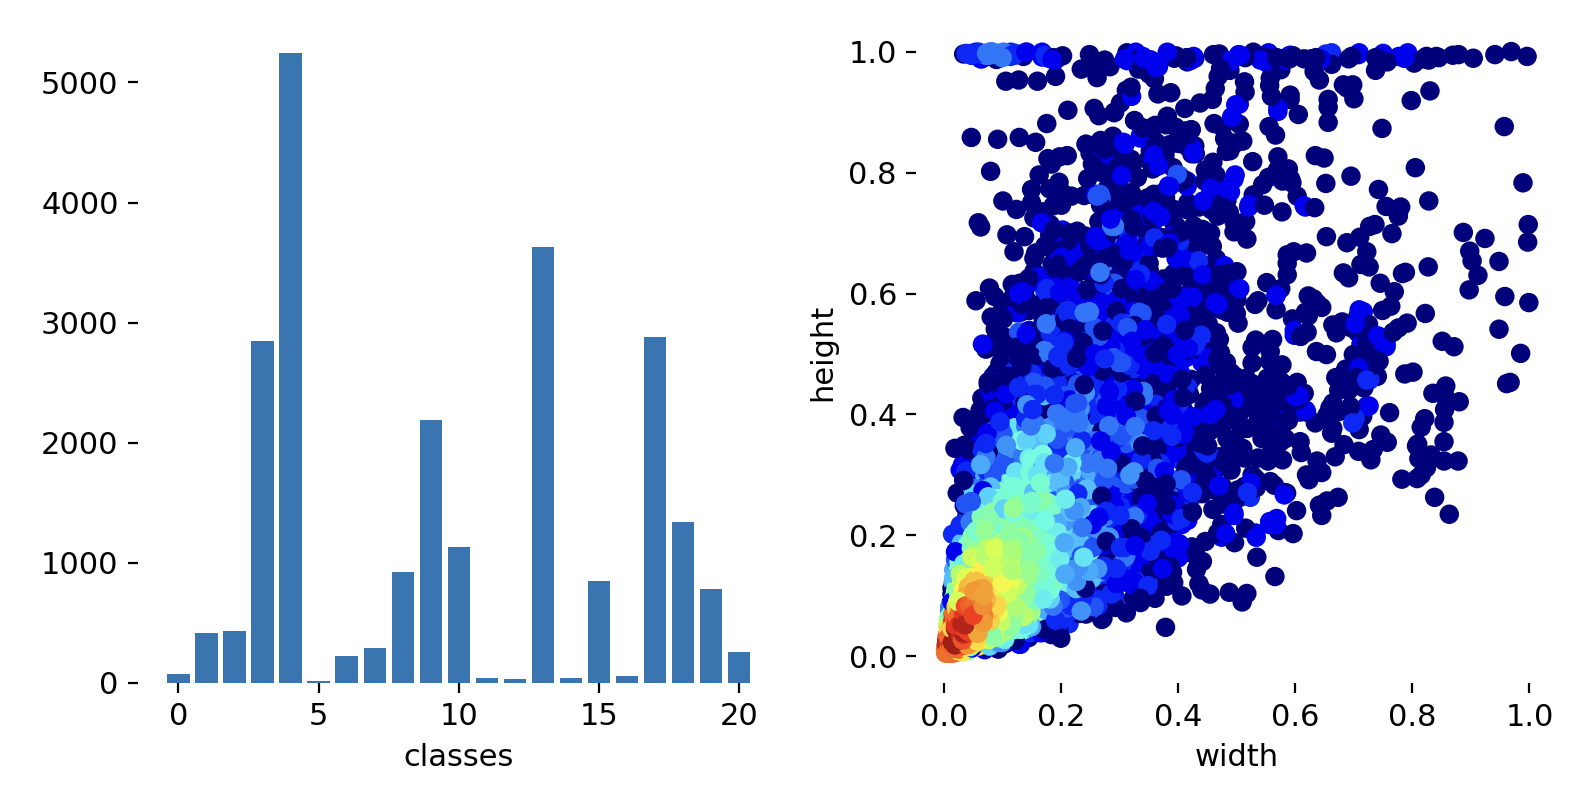
\includegraphics[width=\textwidth]{figures/paper/dhaka-ai+idd.png}
  \caption[Dataset Collage]{\textbf{Dataset Collage}. Some sample data from Dhaka AI dataset.}
  \label{fig:figures/paper/dhaka-ai+idd.png}
\end{figure}


\begin{figure}[H] % \begin{figure}[H] for forcing the figure placement here ; in the bottom, \begin{figure}[!b] ; top of the page, \begin{figure}[!t] ; otherwise, \begin{figure} will let LaTeX decide the best figure placement for you
  \centering
  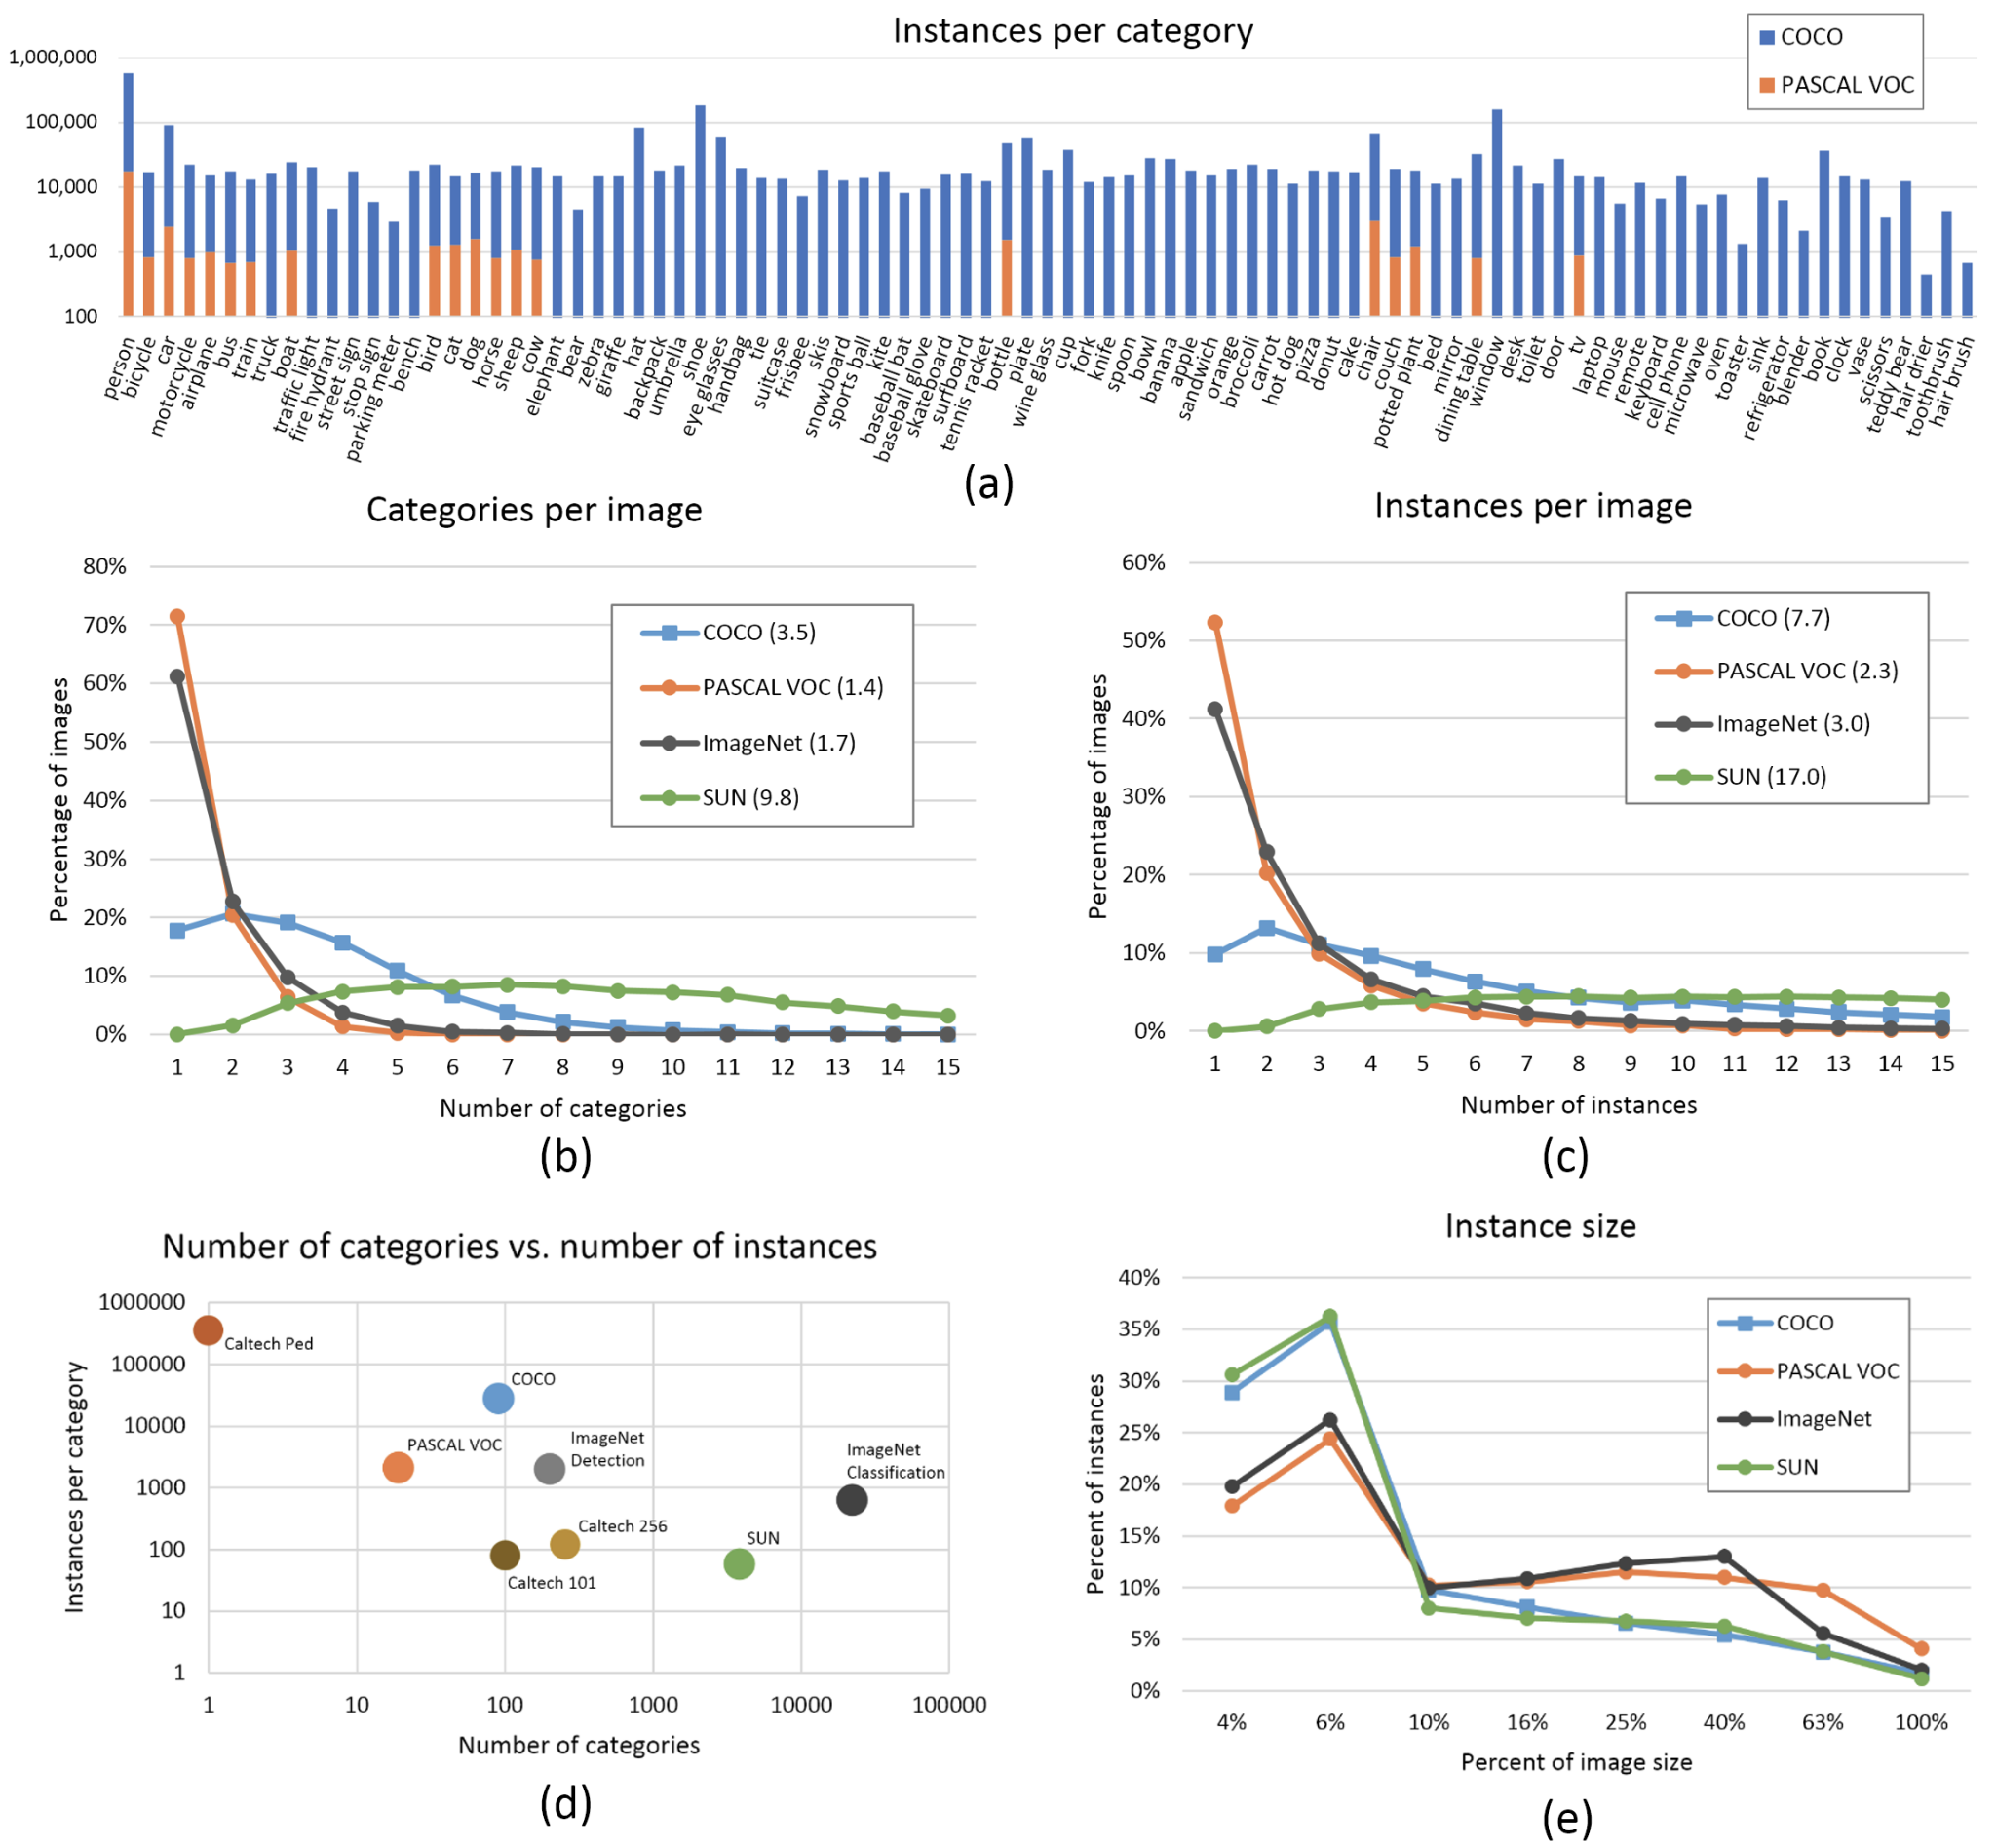
\includegraphics[width=\textwidth]{figures/paper/coco-details.png}
  \caption[Dataset Collage]{\textbf{Dataset Collage}. Some sample data from Dhaka AI dataset.}
  \label{fig:figures/paper/coco-details.png}
\end{figure}



\subsection{List of classes}
\begin{multicols}{2}
\begin{itemize}
\item Ambulance
\item Auto Rickshaw
\item Bicycle
\item Bus
\item Car
\item Garbage Van
\item Human Hauler
\item Minibus
\item Minivan
\item Motorbike
\item Pickup
\item Army Vehicle
\item Police Car
\item Rickshaw
\item Scooter
\item SUV
\item Taxi
\item Three Wheelers (CNG)
\item Truck
\item Van
\item Wheelbarrow
\end{itemize}
\end{multicols}


\section{Training Settings}
Before modifying anything, first train with default settings to establish a performance baseline. A full list of train.py settings can be found in the train.py argparser.
\begin{itemize}
  \item \textbf{Epochs} Start with 300 epochs. If this overfits early then you can reduce epochs. If overfitting does not occur after 300 epochs, train longer, i.e. 600, 1200 etc epochs.
  \item \textbf{Image size} COCO trains at native resolution of \texttt{--img 640}, though due to the high amount of small objects in the dataset it can benefit from training at higher resolutions such as \texttt{--img 1280}. If there are many small objects then custom datasets will benefit from training at native or higher resolution. Best inference results are obtained at the same \texttt{--img} as the training was run at, i.e. if you train at \texttt{--img 1280} you should also test and detect at \texttt{--img 1280}.
  \item \textbf{Batch size} Use the largest \texttt{--batch-size} that your hardware allows for. Small batch sizes produce poor batchnorm statistics and should be avoided.
  \item \textbf{Hyperparameters} Default hyperparameters are in \texttt{hyp.scratch.yaml}. We recommend you train with default hyperparameters first before thinking of modifying any. In general, increasing augmentation hyperparameters will reduce and delay overfitting, allowing for longer trainings and higher final mAP. Reduction in loss component gain hyperparameters like \texttt{hyp['obj']} will help reduce overfitting in those specific loss components.
\end{itemize}


%=======================================================================
%%% References

% \clearpage
\phantomsection
\specialsection % put an indent, see preamble
\headerspecialsection

{\hypersetup{urlcolor=ntnu,linkcolor=sophia} % set clickable URL title color to black, not ntnu like in the main document

  \bibliographystyle{unsrtnat-mod}  % NATBIB ref style
  \bibliography{references}
}

 \chapter[The Training]{The Training}
\markboth{Chap. 3\ \ \enspace Experimental methods}{Chap 2. Experimental methods}

\regularsection
\headerregularsection

\updatemylof % to be used with "list of figure divider per chapter" (see PREAMBLE)
\updatemylot % to be used with "list of table divider per chapter" (see PREAMBLE)

\begin{sloppypar} % to suppress overfull box
In brief the trainng process is:

\begin{itemize}
    \item First, pretrain the first 20 convolutional layers using the ImageNet 1000-class competition dataset, using a input size of 224x224
    \item Then, increase the input resolution to 448x448
    \item Train the full network for about 135 epochs using a batch size of 64, momentum of 0.9 and decay of 0.0005
    \item Learning rate schedule: for the first epochs, the learning rate was slowly raised from 0.001 to 0.01. Train for about 75 epochs and then start decreasing it.
    \item Use data augmentation with random scaling and translations, and randomly adjusting exposure and saturation.
\end{itemize}

\end{sloppypar}



\section{Training Settings}
Before modifying anything, first train with default settings to establish a performance baseline. A full list of train.py settings can be found in the train.py argparser.
\begin{itemize}
\item Epochs. Start with 300 epochs. If this overfits early then you can reduce epochs. If overfitting does not occur after 300 epochs, train longer, i.e. 600, 1200 etc epochs.
\item Image size. COCO trains at native resolution of \texttt{--img 640}, though due to the high amount of small objects in the dataset it can benefit from training at higher resolutions such as \texttt{--img 1280}. If there are many small objects then custom datasets will benefit from training at native or higher resolution. Best inference results are obtained at the same \texttt{--img} as the training was run at, i.e. if you train at \texttt{--img 1280} you should also test and detect at \texttt{--img 1280}.
\item Batch size. Use the largest \texttt{--batch-size} that your hardware allows for. Small batch sizes produce poor batchnorm statistics and should be avoided.
\item Hyperparameters. Default hyperparameters are in \texttt{hyp.scratch.yaml}. We recommend you train with default hyperparameters first before thinking of modifying any. In general, increasing augmentation hyperparameters will reduce and delay overfitting, allowing for longer trainings and higher final mAP. Reduction in loss component gain hyperparameters like \texttt{hyp['obj']} will help reduce overfitting in those specific loss components.
\end{itemize}




\section{Ensemble}
Ensemble modeling is a process where multiple diverse models are created to predict an outcome, either by using many different modeling algorithms or using different training data sets. The ensemble model then aggregates the prediction of each base model and results in once final prediction for the unseen data. The motivation for using ensemble models is to reduce the generalization error of the prediction. As long as the base models are diverse and independent, the prediction error of the model decreases when the ensemble approach is used. The approach seeks the wisdom of crowds in making a prediction. Even though the ensemble model has multiple base models within the model, it acts and performs as a single model. Most of the practical data mining solutions utilize ensemble modeling techniques. \cite{KOTU201517}





%=======================================================================
%%% References

% \clearpage
\phantomsection
\specialsection % put an indent, see preamble
\headerspecialsection

{\hypersetup{urlcolor=ntnu,linkcolor=sophia} % set clickable URL title color to black, not ntnu like in the main document

  \bibliographystyle{unsrtnat-mod}  % NATBIB ref style
  \bibliography{references}
}

 \chapter[Limitations]{Limitations}
\markboth{Chap. 3\ \ \enspace Experimental methods}{Chap 2. Experimental methods}

\regularsection
\headerregularsection

\updatemylof % to be used with "list of figure divider per chapter" (see PREAMBLE)
\updatemylot % to be used with "list of table divider per chapter" (see PREAMBLE)

\begin{sloppypar} % to suppress overfull box
YOLO imposes strong spatial constraints on boundingbox predictions since each grid cell only predicts two boxes and can only have one class. This spatial constraint limits the number of nearby objects that our model can predict. Our model struggles with small objects that appear ingroups, such as flocks of birds.Since our model learns to predict bounding boxes fromdata, it struggles to generalize to objects in new or unusual aspect ratios or configurations. Our model also uses relatively coarse features for predicting bounding boxes since our architecture has multiple downsampling layers from the input image.Finally, while we train on a loss function that approximates detection performance, our loss function treats errors the same in small bounding boxes versus large bounding boxes. A small error in a large box is generally benign but a small error in a small box has a much greater effect on IOU.Our main source of error is incorrect localizations.
\end{sloppypar}



%=======================================================================
%%% References

% \clearpage
\phantomsection
\specialsection % put an indent, see preamble
\headerspecialsection

{\hypersetup{urlcolor=ntnu,linkcolor=sophia} % set clickable URL title color to black, not ntnu like in the main document

  \bibliographystyle{unsrtnat-mod}  % NATBIB ref style
  \bibliography{references}
}

 \chapter[Result and Analysis]{Result and Analysis}
\markboth{Chap. 3\ \ \enspace Experimental methods}{Chap 2. Experimental methods}

\regularsection
\headerregularsection

\updatemylof % to be used with "list of figure divider per chapter" (see PREAMBLE)
\updatemylot % to be used with "list of table divider per chapter" (see PREAMBLE)

\begin{sloppypar} % to suppress overfull box
Here we will compare our model with existing models and our proposed model result. We tried this dataset in 5 different models: 
\end{sloppypar}



\begin{table}[!h]
  \centering
  \caption[YOLO Network Structure]{YOLO Network Structure}
  \label{tab:yolo-network}
  {\renewcommand{\arraystretch}{1.7}
      \begin{tabular}{p{4cm} p{1cm} p{0.8cm} p{1cm} p{2.6cm}}
          \toprule
          Model Name                                    & mAP (our dataset) & COCO mAP & Speed (ms) & Detect Small object and less overlapping \\
          \hline
          EfficientDet D4 1024x1024                     & 12.27             & 48.5     & 133        & YES                                      \\
          SSD ResNet152 V1 FPN 1024x1024 (RetinaNet152) & 8.75              & 38.3     & 104        & NO                                       \\
          Faster R-CNN ResNet101 V1 1024x1024           & 11.56             & 37.1     & 72         & NO                                       \\
          Faster R-CNN Inception ResNet V2 1024x1024    & 11.89             & 38.7     & 236        & NO                                       \\
          YOLO v5(1024x1024)                            & 12.06             & 49.7     & 65         & YES                                      \\
          YOLO v5(1024x1024) Modified (Proposed Method) & 13.46             & 49.8     & 70         & YES                                      \\
          \bottomrule
    \end{tabular}
  }
\end{table}

After benchmarking with above model we found that our model do best both in time and accuracy.

The dataset in the start is labelled for 21 classes {Ambulance, Auto Rickshaw, Bicycle, Bus, Car, Garbage Van, Human Hauler, Minibus, Minivan, Motorbike, Pickup, Army Vehicle, Police Car, Rickshaw, Scooter, SUV, Taxi, Three Wheelers (CNG), Truck, Van, Wheelbarrow} and has been trained for 60 epochs using the network configuration of~\ref{tab:yolo-parameter}.  The  network  has been  trained  for  60  epochs  that  are  20000  iterations  (4 epochs  are
1328 iterations) because darknet framework trains a maximum of 2000 iterations for each class
and calculates the mAP@0.5 every 4 epochs for the validation set and every 3 epochs for the
test set unless the difference between the cost of an iteration and the cost of the next iteration
is lower than 0.0005.


\begin{table}[!h]
  \centering
  \caption[Initial values for the YOLO network parameters.]{Initial values for the YOLO network parameters.}
  \label{tab:yolo-parameter}
  {\renewcommand{\arraystretch}{1.7}
    \begin{tabular}{p{6.5cm} p{4cm}}
          \toprule
          Parameter                                                                         & Value  \\
          \hline
          Batch size                                                                        & 64 \\ 
          Subdivisions = sub batches: number of mini batches it is split up the batch       & 32 \\
          Width $\times$ height of the input images                                         & 416 $\times$ 416  \\
          IoU minimum threshold between predicted BB and ground-truth                       & 0.5 \\
          Data augmentation                                                                 & Saturation and exposure=1.5 angle=0 hue=0.1  \\
          Learning rate                                                                     & 0.001 \\
          Max\_batches                                                                      & Number class $\times$ 2000 \\
          Momentum                                                                          & 0.9 \\
          Decay                                                                             & 0.0005 \\
          \bottomrule
    \end{tabular}
  }
\end{table}

\begin{table}[!h]
  \centering
  \caption[Evaluation of the model]{Evaluation of the model on the validation set with an IoU threshold of 50% that is the 
Area-Under-Curve for each unique Recall. }
  \label{tab:class-ap}
  {\renewcommand{\arraystretch}{1.7}
    \begin{tabular}{p{1.5cm} p{1.5cm} p{1.5cm} p{1.5cm} p{1.5cm} p{1.5cm}}
          \toprule
          Epochs & Ap Car & Ap Rickshaw & Ap  Bus & Ap SUV & Ap Truck \\
          \hline
          3 & 39.35\% & 09.33\% & 39.57\% & 16.76\% & 27.82\% \\
          6 & 41.65\% & 13.68\% & 41.73\% & 18.74\% & 30.76\% \\ 
          9 & 44.15\% & 15.01\% & 43.53\% & 19.02\% & 32.07\% \\
          12 & 48.35\% & 15.93\% & 46.98\% & 19.38\% & 33.43\% \\
          15 & 49.89\% & 16.45\% & 50.13\% & 20.31\% & 34.76\% \\
          \bottomrule
    \end{tabular}
  }
\end{table}

For evaluating which weight file is the best one to use for detecting vehicles in new images we 
will guide by the mAP value computed in the validation and test set. In the~\ref{tab:class-ap} we can 
see which weights files give best value on the mAP. The training has been done for 15 epochs, 
but  it  can  happen  that  the  weights  computed  in  previous  epochs  give  a  better  value  on  the 
precision and the mAP. This may happen due to overfitting; the model is very good detecting on 
the training set but falls to detect objects in new images. As it can be seen in Table 4, the weight 
file  stored in the epoch 15 and the epoch 18 obtain the  best mAP value of 37.20\% and in the 
Table 3 the weight file obtained in the epoch 16 gets a 35.52\% mAP best value.  

%\begin{figure}[H] % \begin{figure}[H] for forcing the figure placement here ; in the bottom, \begin{figure}[!b] ; top of the page, \begin{figure}[!t] ; otherwise, \begin{figure} will let LaTeX decide the best figure placement for you
%    \begin{minipage}{0.45\textwidth}
%  \centering
%  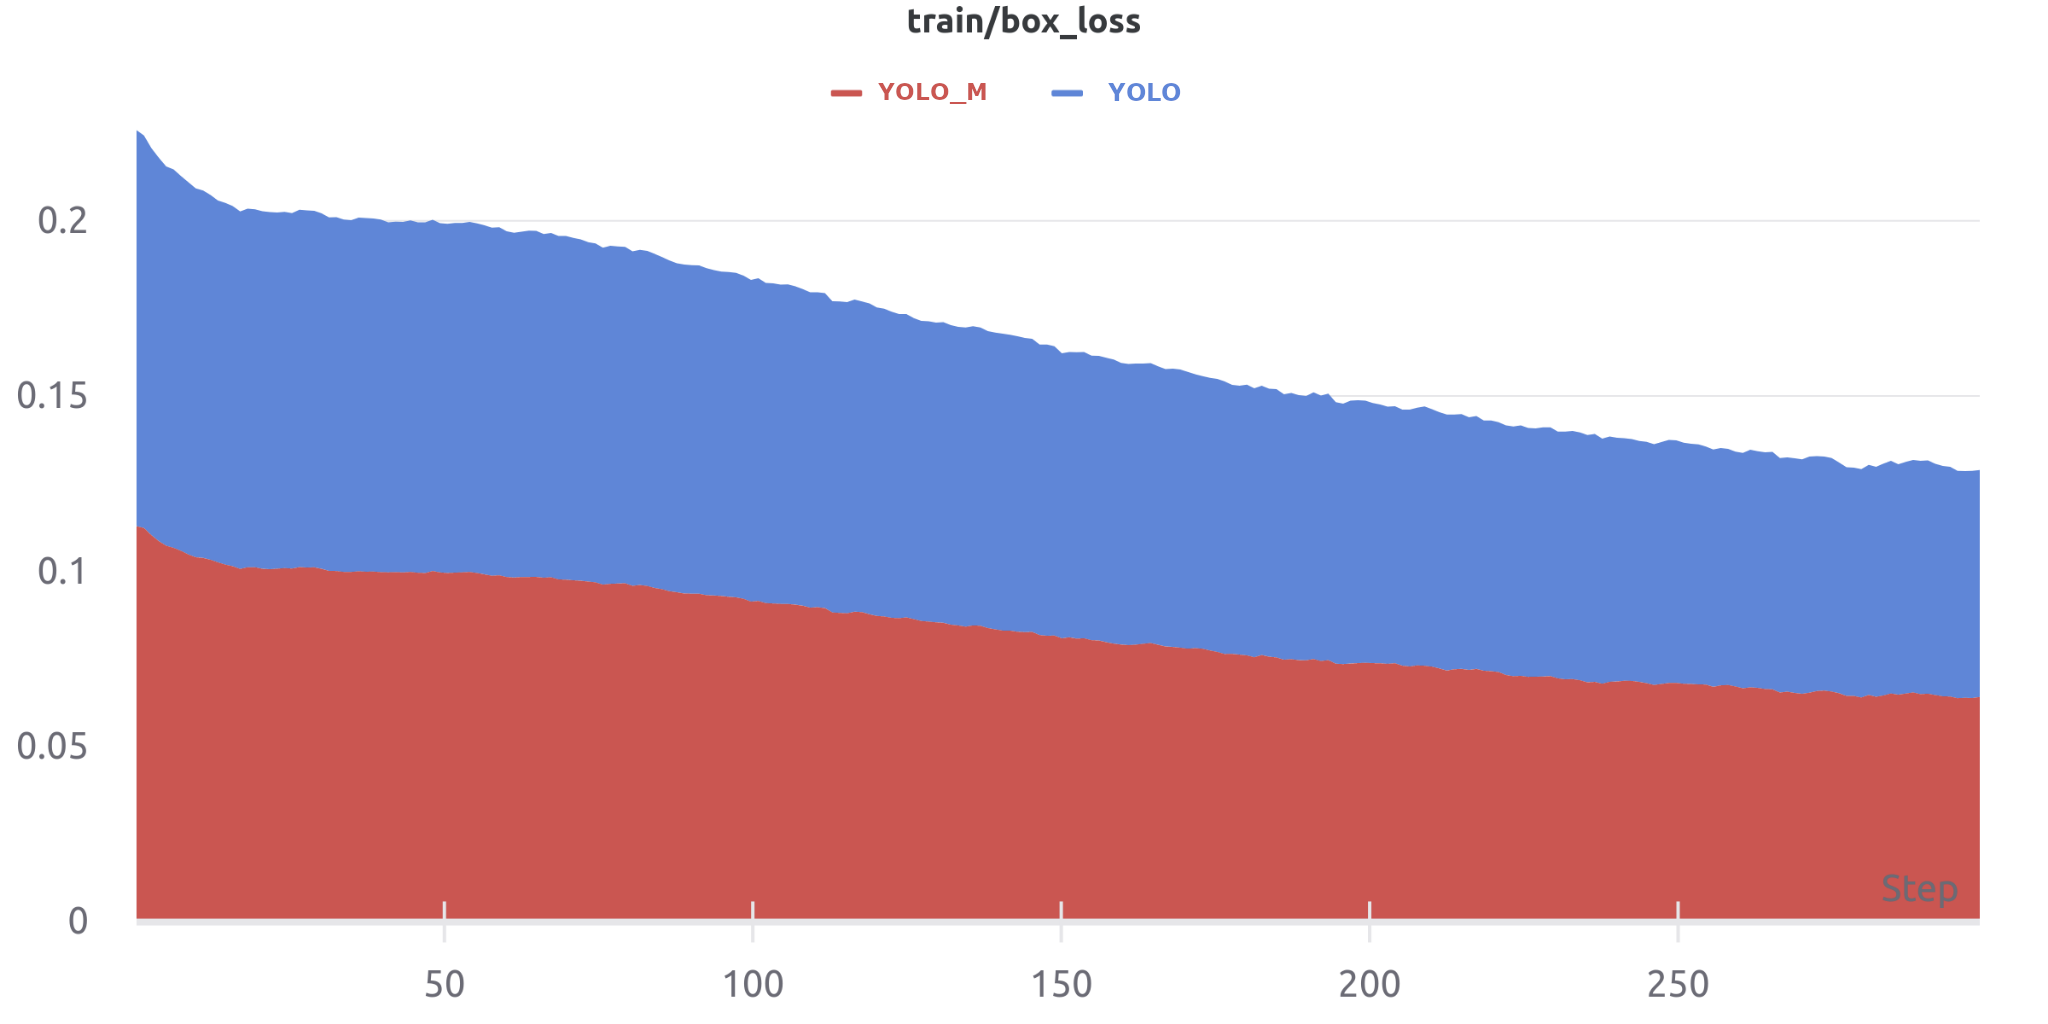
\includegraphics[width=0.9\textwidth]{figures/paper/box-loss.png}
%  \caption[The Architecture]{\textbf{The Architecture}. }
%  \label{fig:figures/paper/box-loss}
%  \end{minipage}\hfill
%%\end{figure}


%%\begin{figure}[H] % \begin{figure}[H] for forcing the figure placement here ; in the bottom, \begin{figure}[!b] ; top of the page, \begin{figure}[!t] ; otherwise, \begin{figure} will let LaTeX decide the best figure placement for you
%  \begin{minipage}{0.45\textwidth}
%  \centering
%  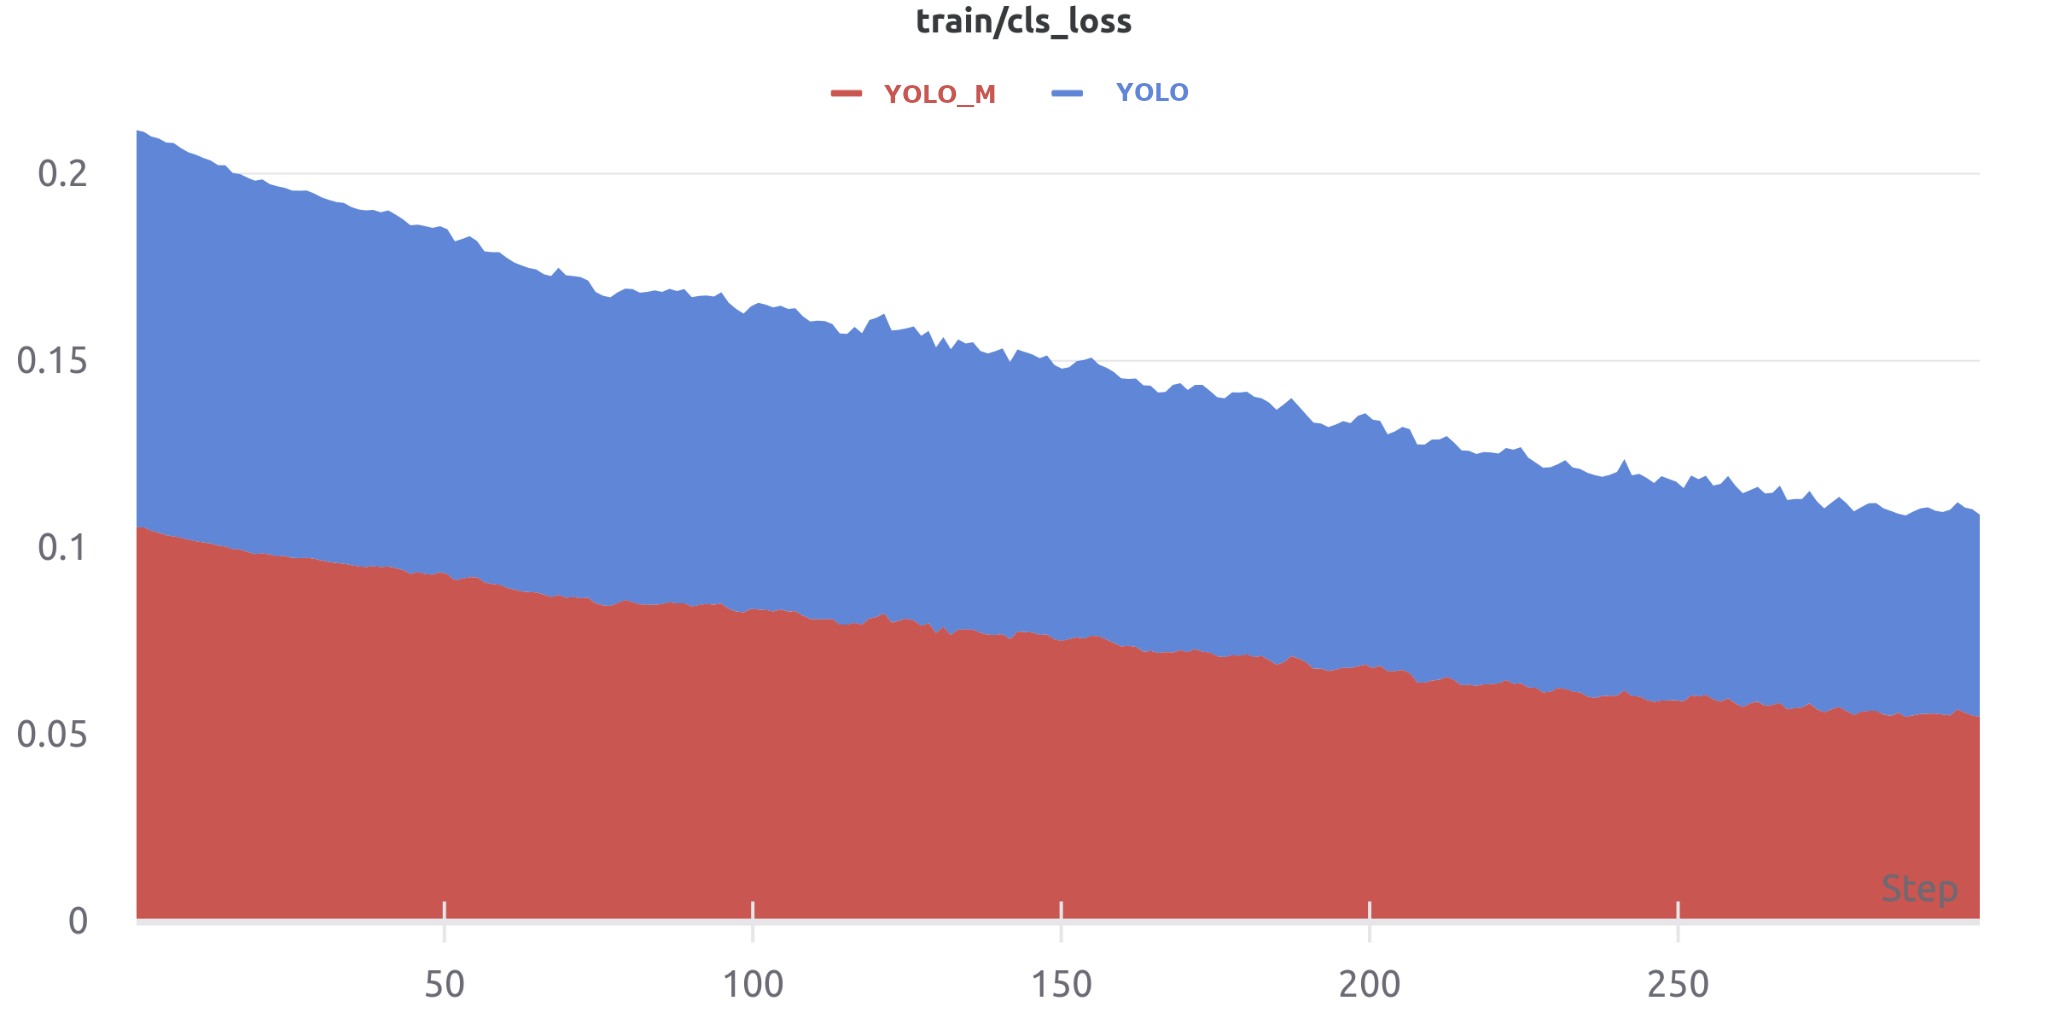
\includegraphics[width=0.9\textwidth]{figures/paper/cls-loss.png}
%  \caption[The Architecture]{\textbf{The Architecture}. }
%  \label{fig:figures/paper/cls-loss}
%  \end{minipage}
%\end{figure}


\begin{figure}
    \centering
    \begin{minipage}{0.48\textwidth}
        \centering
  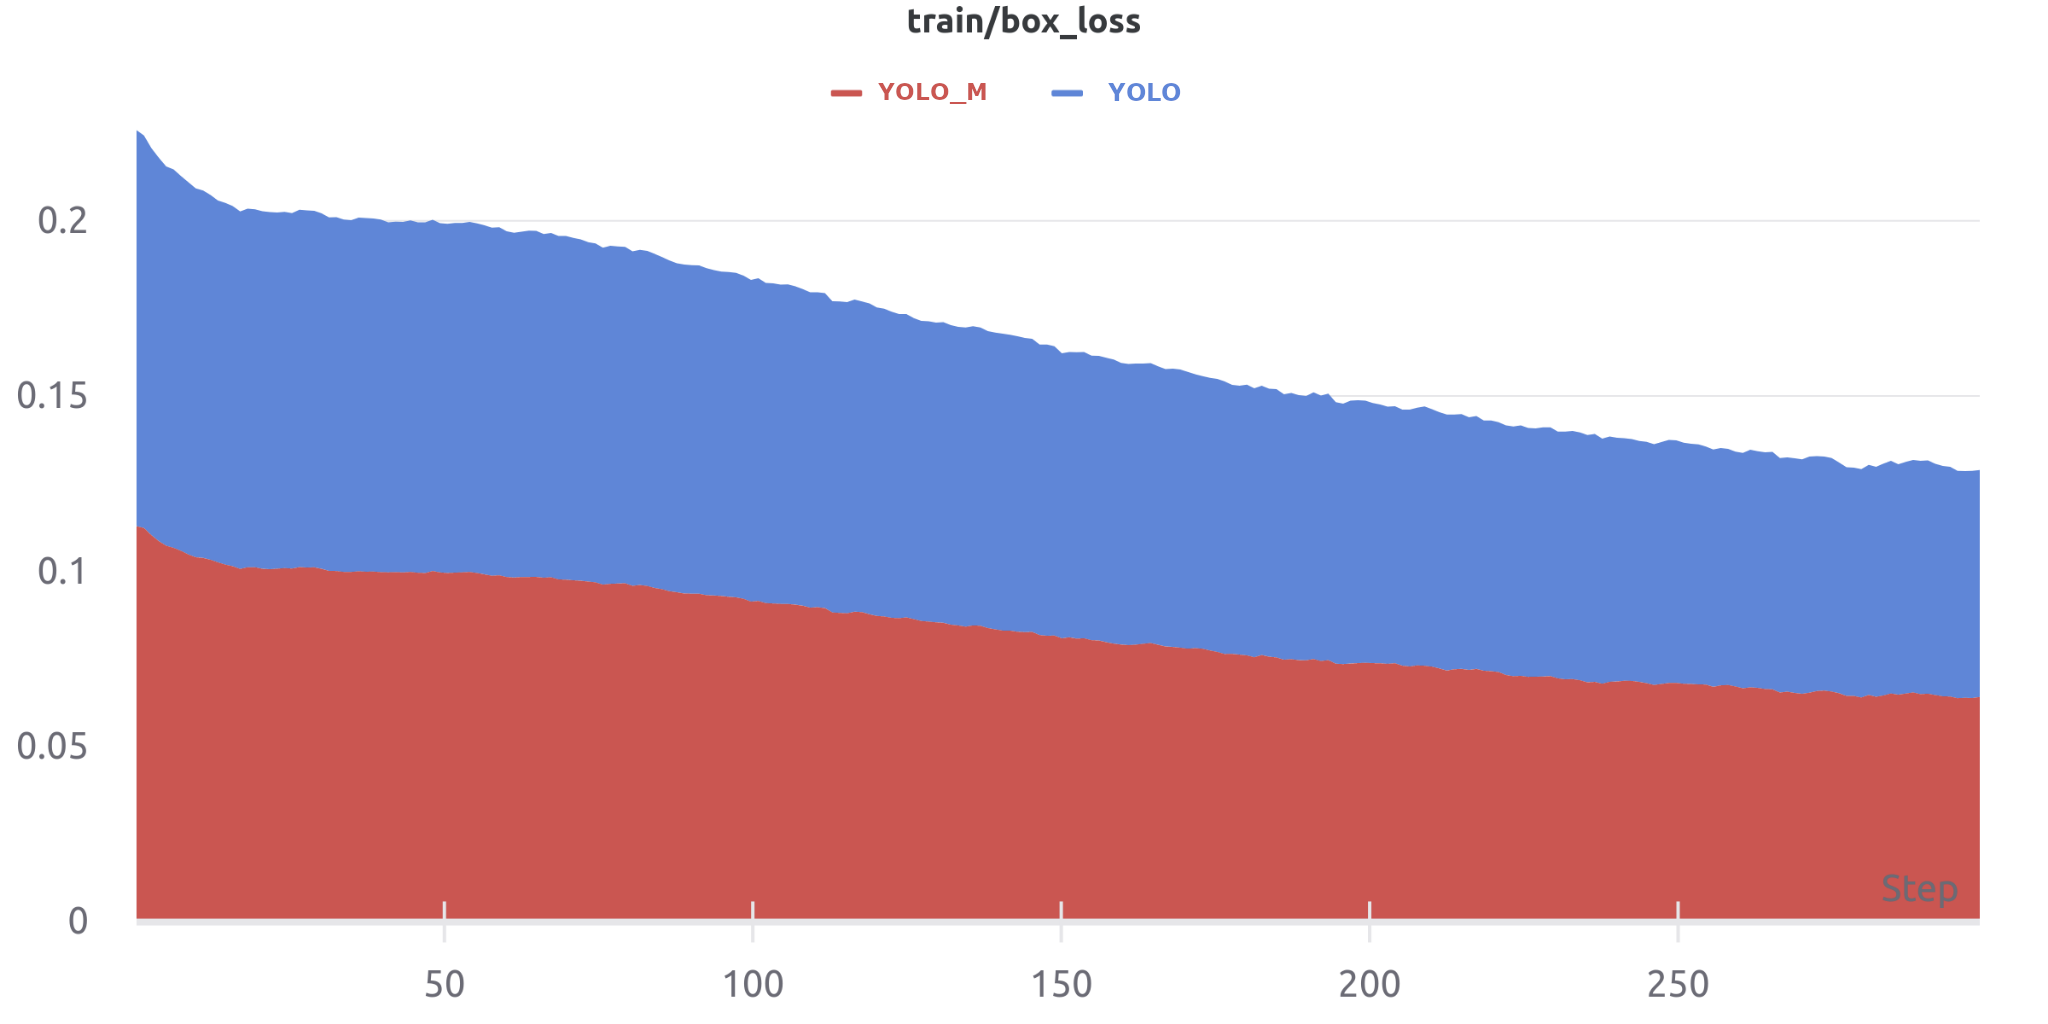
\includegraphics[width=\textwidth]{figures/paper/box-loss.png}
    \end{minipage}\hfill
    \begin{minipage}{0.48\textwidth}
        \centering
  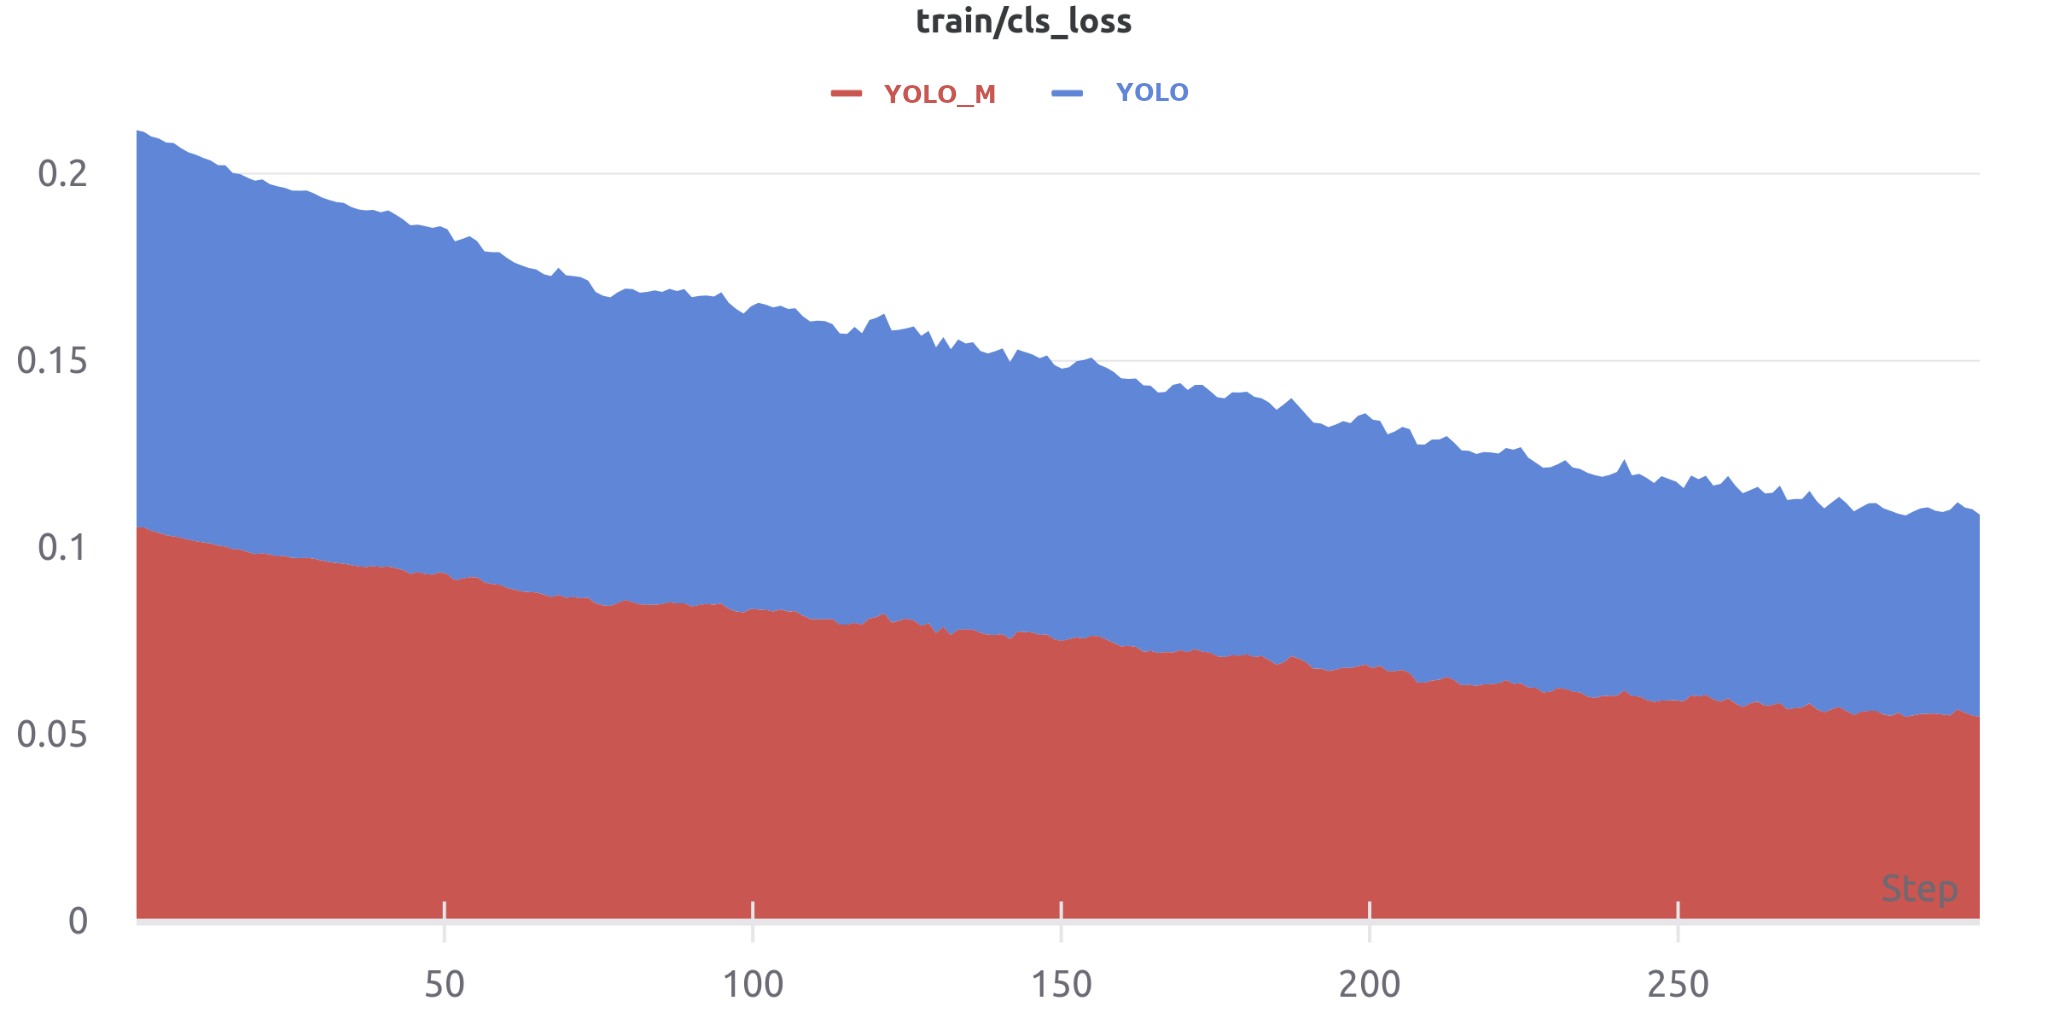
\includegraphics[width=\textwidth]{figures/paper/cls-loss.png}
    \end{minipage}
    \caption[Box loss and Classificaton loss]{\textbf{Losses over Epochs} Box loss and Classificaton loss }
  \label{fig:figures/paper/box-loss}
\end{figure}






\begin{figure}[H] % \begin{figure}[H] for forcing the figure placement here ; in the bottom, \begin{figure}[!b] ; top of the page, \begin{figure}[!t] ; otherwise, \begin{figure} will let LaTeX decide the best figure placement for you
  \centering
  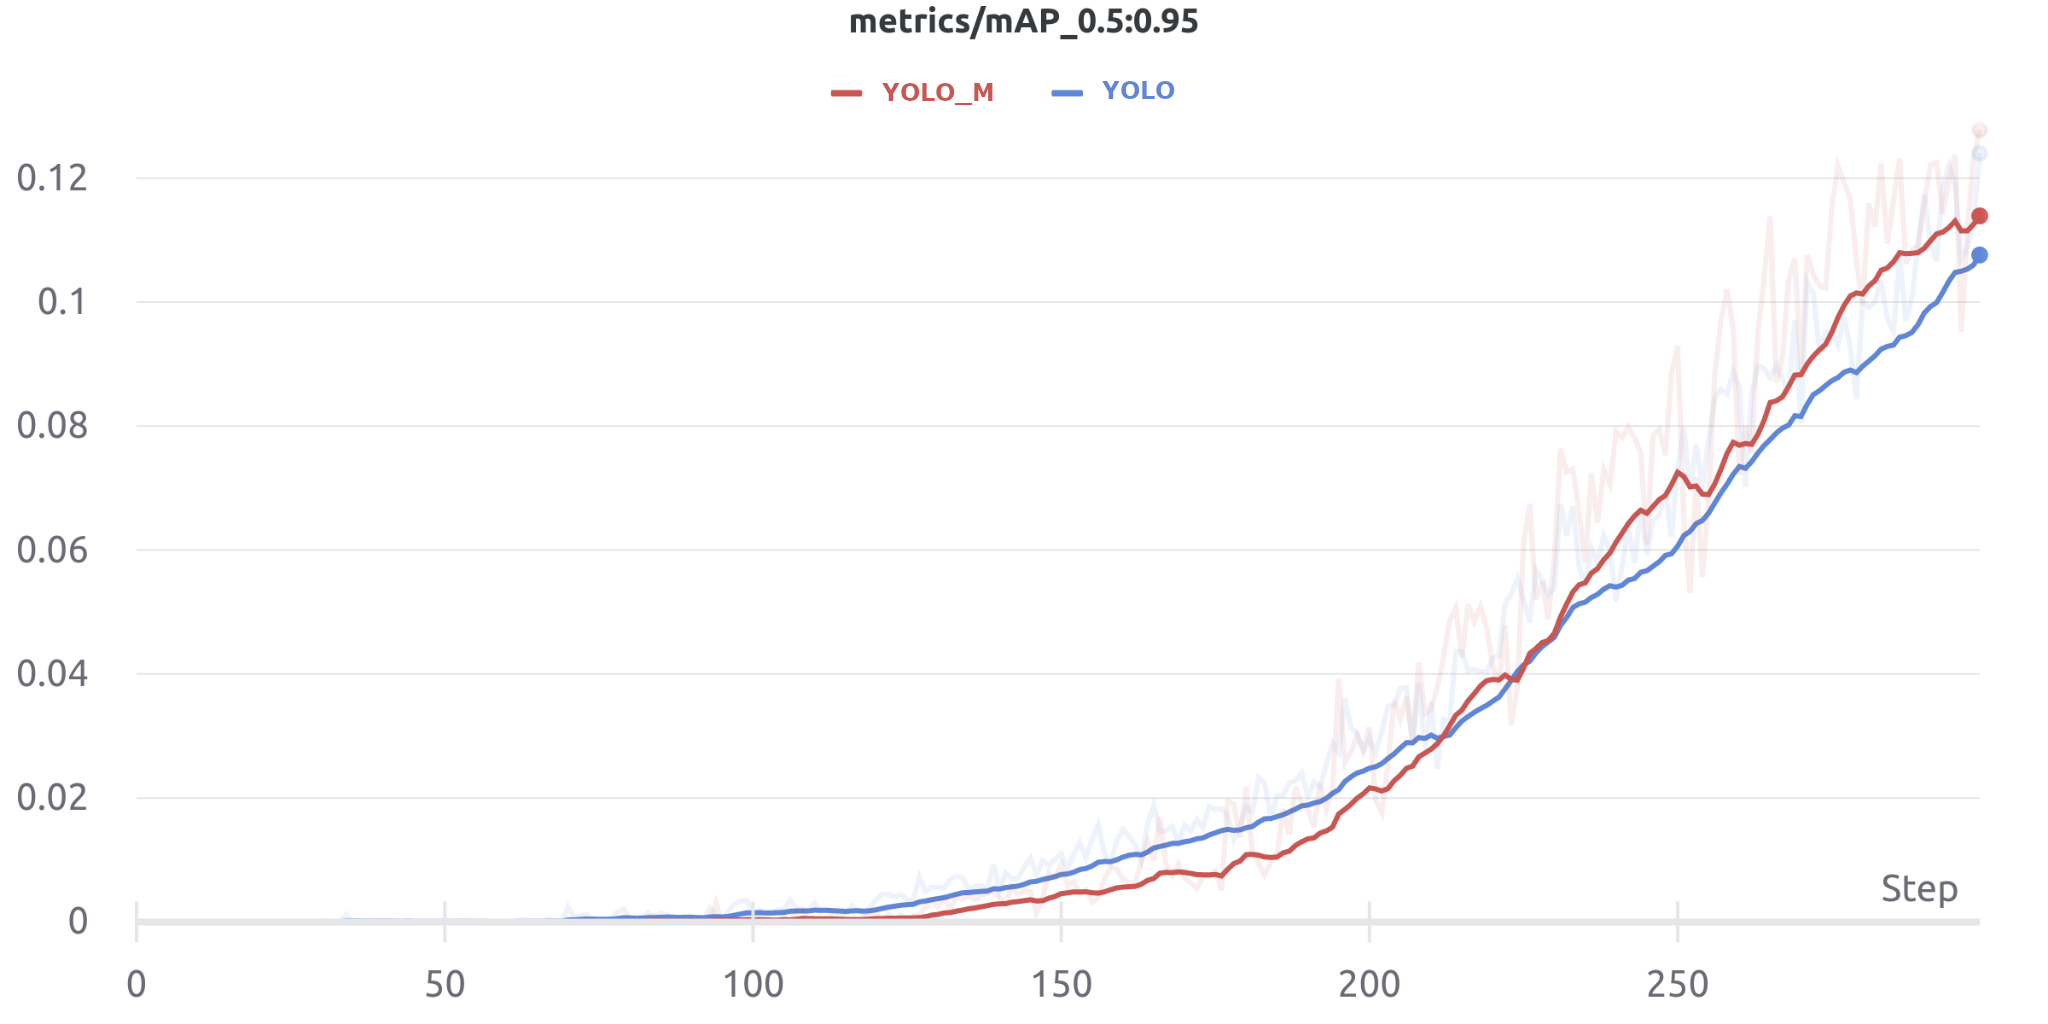
\includegraphics[width=\textwidth]{figures/paper/mAP.png}
  \caption[The Architecture]{\textbf{mAP Comparison of YOLOv5 and Modified YOLO with ORB}. Graph computed during the training; the mAP is computed over the validation set.}
  \label{fig:figures/paper/mAP}
\end{figure}

In the~\ref{fig:figures/paper/mAP} we can see the graph that shows the average loss computed for every iteration
and  the  mAP  calculated  for  every  4  epochs  (1  epoch  =  332  iterations  so  4  epochs  =  1328
iterations). The value of the  loss remains between 3.5 and 4  and the mAP has a value of 35\%
from the iteration 5000 (epoch 15) to the iteration 6000 (epoch 18). With the~\ref{fig:figures/paper/mAP}
and the~\ref{tab:class-ap} we can conclude that the best weight file for detecting vehicles in new
images is obtained in the epoch 15. Note that the dataset is quite complex as it has many
labelled small vehicles in each images that are not visually easy to see, this complexity affects
the mAP value by obtaining a relatively low one. This happens because the model fails to detect
some vehicles in the validation set that it is difficult even for the human eye to detect them. On
the next pages, to test the capability of generalizing of our model for this training, we will get
one image containing cars, other image containing trucks, other image containing motors and a
final image containing cars, trucks and SUVs and pass them from our model to see if it is able
to detect all the vehicles in the images.



\begin{figure}[H] % \begin{figure}[H] for forcing the figure placement here ; in the bottom, \begin{figure}[!b] ; top of the page, \begin{figure}[!t] ; otherwise, \begin{figure} will let LaTeX decide the best figure placement for you
  \centering
  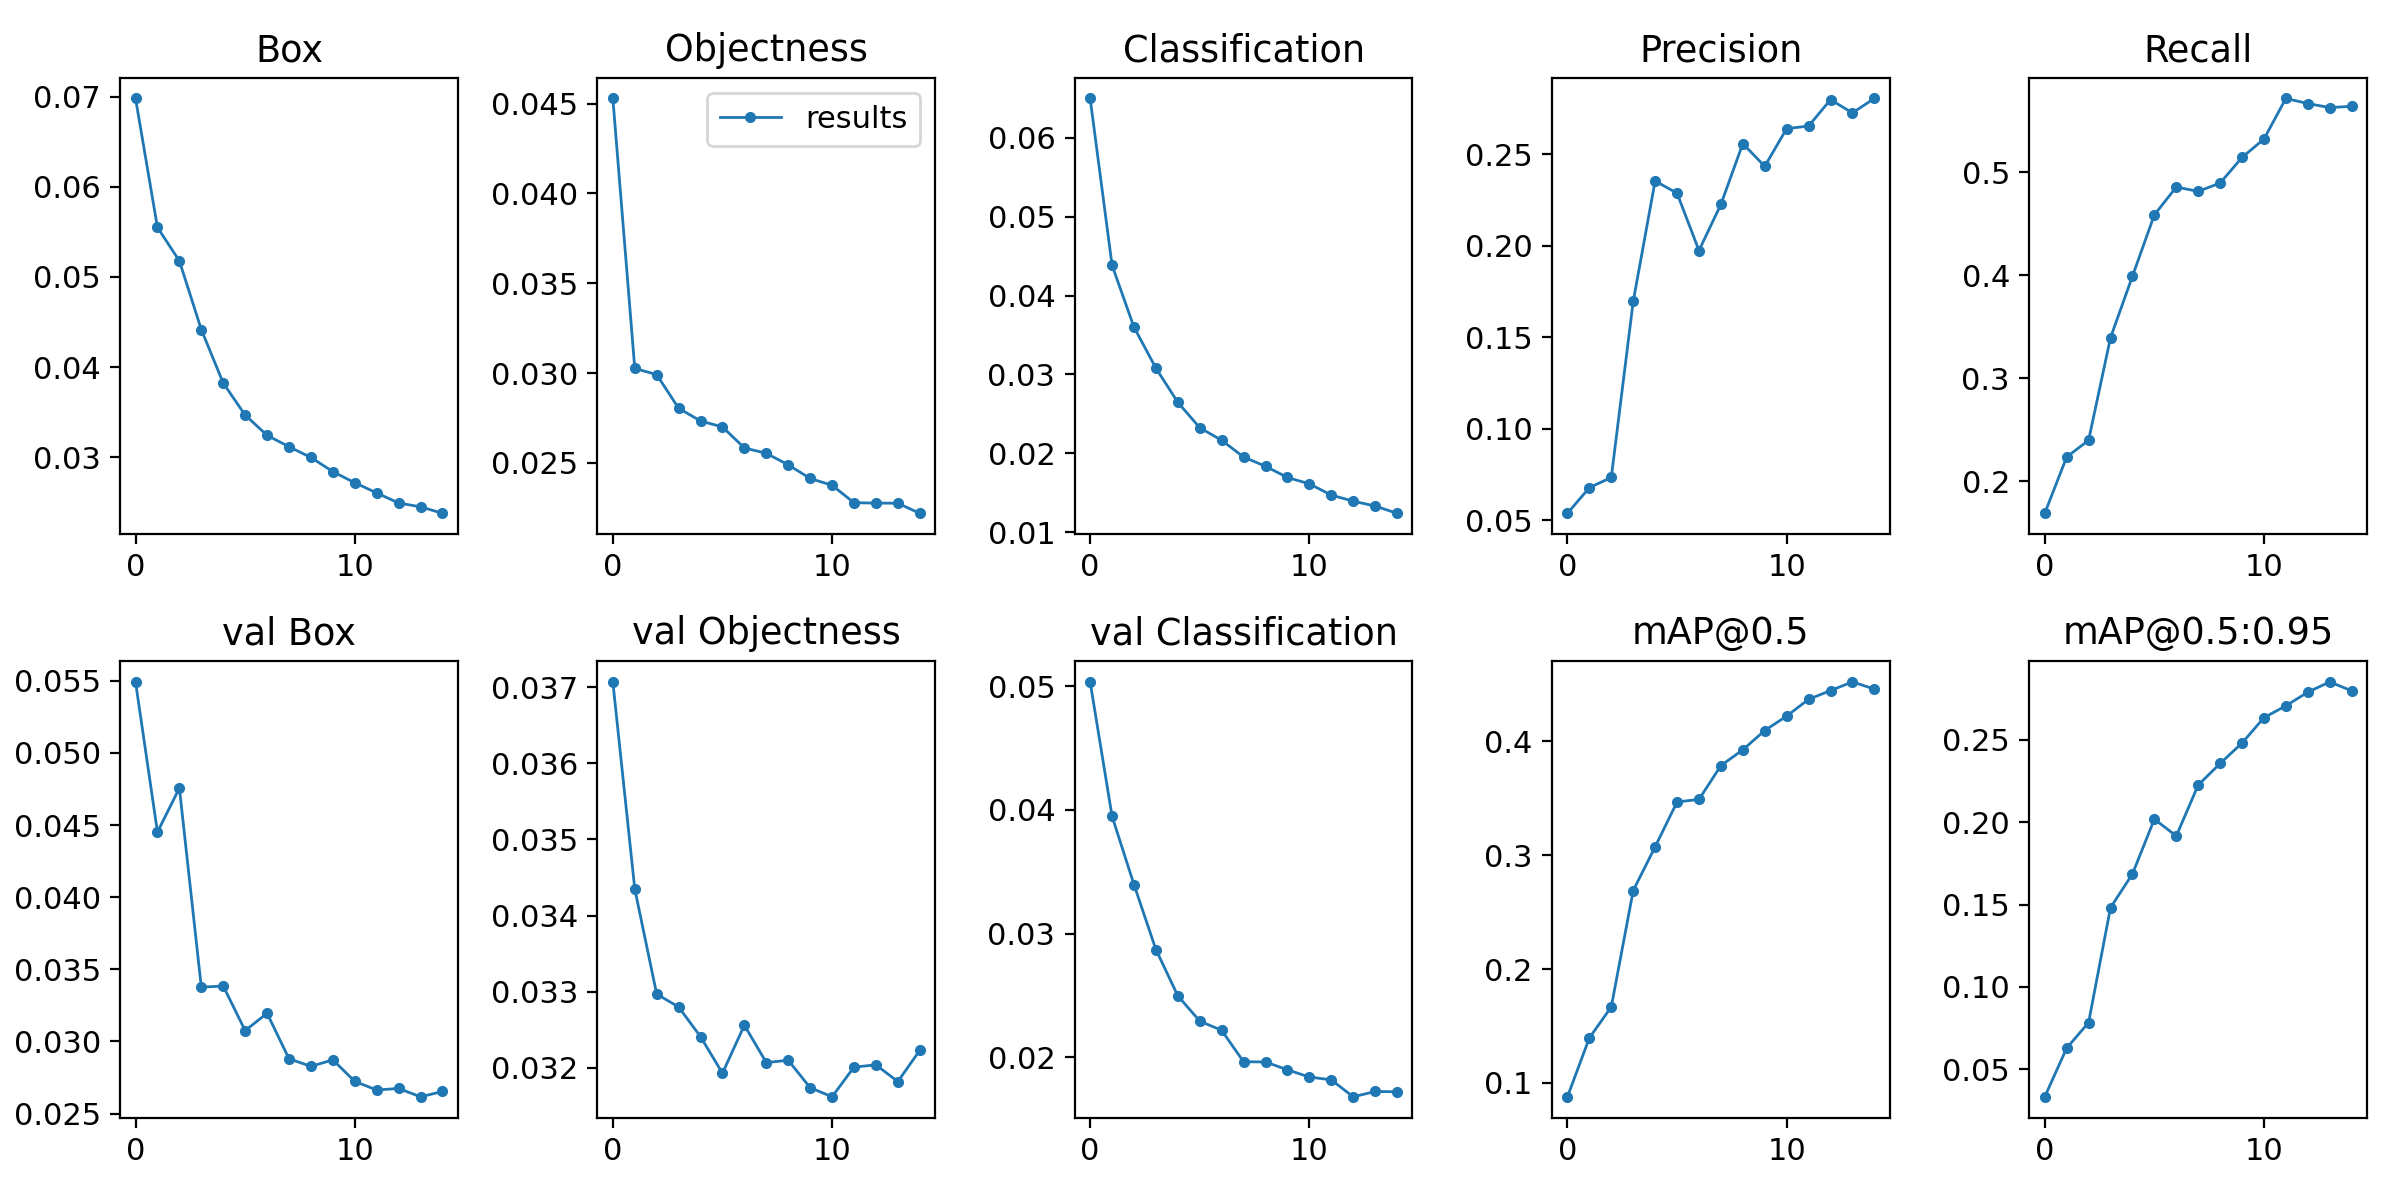
\includegraphics[width=\textwidth]{figures/paper/results.png}
  \caption[The Architecture]{\textbf{Result of Dhaka AI and Indian Driving Dataset}. }
  \label{fig:figures/paper/results}
\end{figure}

\begin{figure}[H] % \begin{figure}[H] for forcing the figure placement here ; in the bottom, \begin{figure}[!b] ; top of the page, \begin{figure}[!t] ; otherwise, \begin{figure} will let LaTeX decide the best figure placement for you
  \centering
  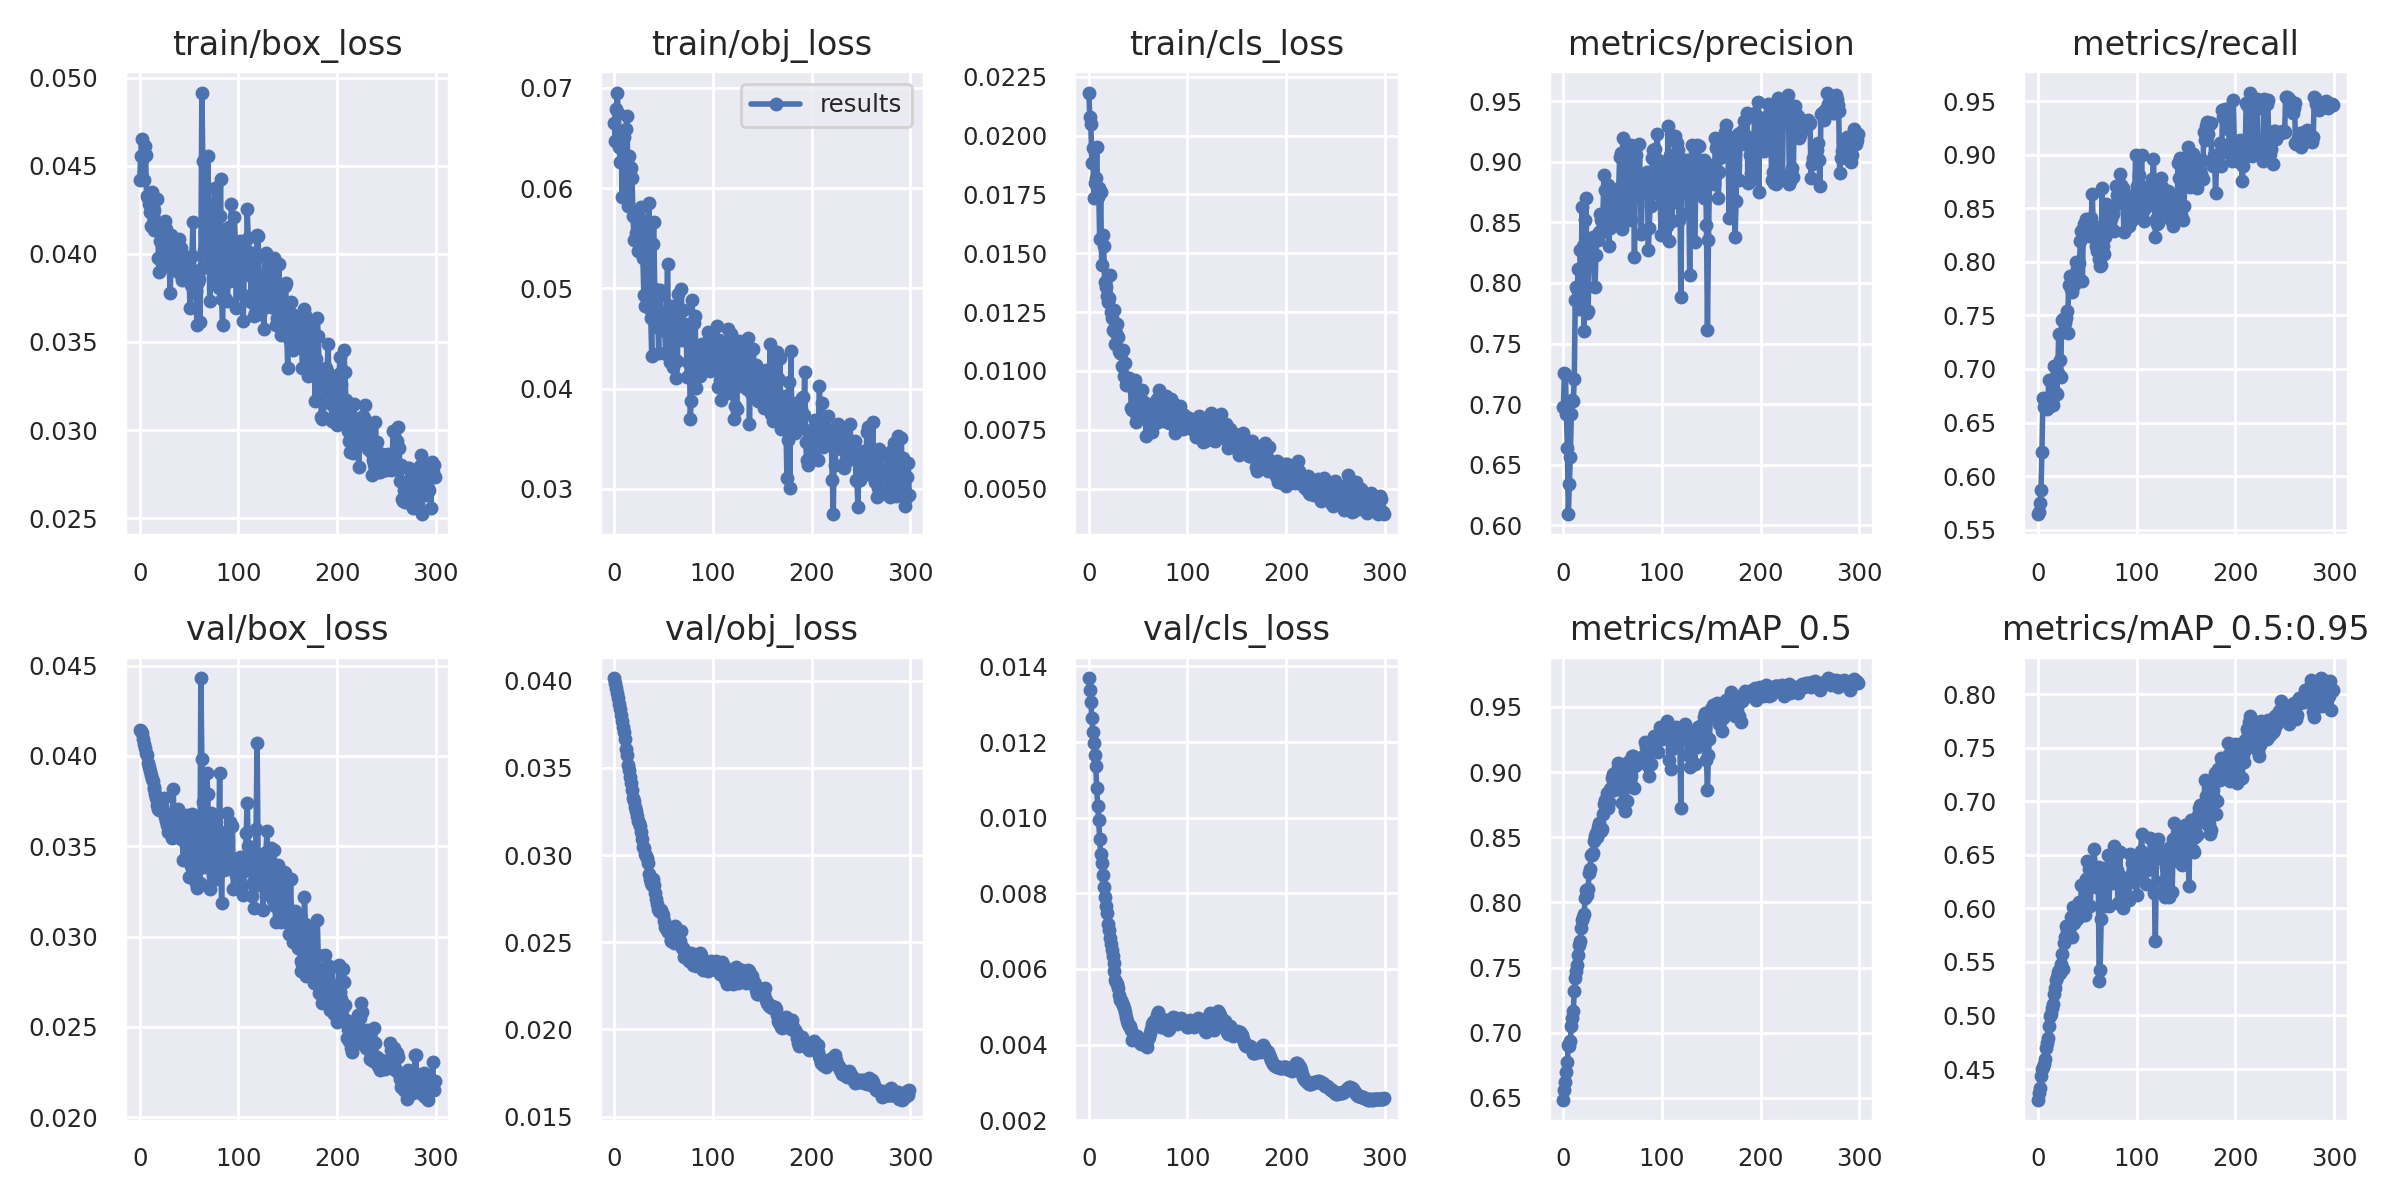
\includegraphics[width=\textwidth]{figures/paper/yolo-on-coco.png}
  \caption[The Architecture]{\textbf{Result on COCO}. }
  \label{fig:figures/paper/yolo-on-coco}
\end{figure}


%=======================================================================
%%% References

% \clearpage
\phantomsection
\specialsection % put an indent, see preamble
\headerspecialsection

{\hypersetup{urlcolor=ntnu,linkcolor=sophia} % set clickable URL title color to black, not ntnu like in the main document

  \bibliographystyle{unsrtnat-mod}  % NATBIB ref style
  \bibliography{references}
}


\cleardoublepage\phantomsection % to fix wrong hyperref to \part{Result}
\part{Results}

% \chapter[Title of the chapter 4 displayed \\ in the table of contents]
    {Title of the chapter 4 displayed in the page
        \chaptermark{Ch. 4 title in the header}
    }
    \chaptermark{Ch. 4 title in the header}
\label{ch:labelchapter4}

\updatemylof % to be used with "list of figure divider per chapter" (see PREAMBLE)

\regularsection
\headerregularsection

Author 1\textsuperscript{1,\textcolor{sophia}{$\ast$}}, Author 2\textsuperscript{1,2,\textcolor{sophia}{$\ast$}}, Author 3\textsuperscript{3}, Author 4\textsuperscript{1}, Author 5\textsuperscript{1}, Author 6\textsuperscript{1}, Author 7\textsuperscript{2,4,\#} and Author 8\textsuperscript{1,\#} \hfill \textcolor{sophia}{\textsuperscript{$\ast$}\textit{Author 1 and Author 2 contributed equally to this study.}} \newline

\let\thefootnote\relax\footnotetext{\textsuperscript{1}Department X, University 1, City A, Country B. 
\textsuperscript{2}Department Y, University 2, City C, Country D. 
\textsuperscript{3}Institute E, City F, Country G. 
\textsuperscript{4}Research Center H, University I, City J, Country K. 
\textsuperscript{\#}e-mail: \href{mailto:author7@university2.ac.countryD}{author7@university2.ac.countryD} and \href{mailto:author8@universityI.countryK}{author8@universityI.countryK}}

\noindent First published in: \textit{Scientific Reports} \textbf{10}, 853 (2020). \hfill \break
DOI: \href{https://doi.org/10.1038/s41598-019-55424-z}{10.1038/s41598-019-55424-z} 

\begin{wrapfigure}[3]{l}{0.2\textwidth}
    
\includegraphics[width=0.2\textwidth]{figures/by.png}
\end{wrapfigure} 

\noindent \textcolor{white}{test} \newline \textbf{Open Access} This article is licensed under a Creative Commons Attribution 4.0 International License. It means that unrestricted use, sharing, adaptation, distribution, and reproduction in any medium or format are allowed, as long as the original author(s) and the source are appropriately credited, a link to the Creative Commons license is provided, and any changes made are indicated. To view a copy of this license, please visit \href{http://creativecommons.org/licenses/by/4.0/}{http://creativecommons.org/licenses/by/4.0/}. \newline

\noindent \copyright \ Liudi Mulyo \textit{et al}, 2020. \newline

\noindent \textbf{Contributions} \newline
\noindent \lipsum[2]

%%%%%%%%%%%%%%%%%%%%%%%%%%%%%%%%%%%%%%%%%%%%%%%%%%%%%%%%%%%%%%%%%%%%%%%%%%%%%%%%%%%%%%%%%%%%%%%%%%%%%%%%%%%%%%%%%%%%%%%%%%%

\tcbset{enhanced,colback=abstractback,colframe=sophia,fonttitle=\bfseries}
\begin{tcolorbox}[left=3.35cm,grow to left by=3.5cm,right=3.33cm,grow to right by=3.5cm,title={\normalfont \color{White} \small \fontfamily{bch} \selectfont \scshape Abstract}]
% https://tex.stackexchange.com/questions/232878/inserting-pictures-in-tcolorbox
% https://tex.stackexchange.com/questions/169794/outer-margin-of-tcolorbox/169877
% https://tex.stackexchange.com/questions/11484/how-to-draw-a-frame-box-around-an-arbitrary-large-piece-of-text-figures-whatever
\begin{minipage}[t]{\linewidth}
\vspace*{-29pt}
\phantomsection % to fix wrong hyperref to "Abstract" 
\section*{} % for linking from TOC (only one way)
\addcontentsline{toc}{section}{Abstract}
\begin{sloppypar}
\lipsum[1]
\end{sloppypar}

\end{minipage}

\vspace*{3.5pt}
\end{tcolorbox}

%%%%%%%%%%%%%%%%%%%%%%%%%%%%%%%%%%%%%%%%%%%%%%%%%%%%%%%%%%%%%%%%%%%%%%%%%%%%%%%%%%%%%%%%%%%%%%%%%%%%%%%%%%%%%%%%%%%%%%%%%%%

\begin{sloppypar} % to suppress overfull box

Lorem \index{Lorem} ipsum dolor sit amet, consectetuer adipiscing elit \cite{LIUDIMULYO201767}. Ut purus \index{purus} elit,vestibulum ut, placerat ac, adipiscing vitae, felis \citenum{LIUDIMULYO201767}. Curabitur dictum \index{dictum} gravidamauris. Nam arcu libero, nonummy eget, consectetuer id, vulputate a, magna. Donec vehicula augue eu neque \cite{liudimulyo_2018}. Pellentesque habitant morbi tristique senectuset netus et malesuada fames ac turpis egestas \index{egestas}\citenum{liudimulyo_2018}. Mauris ut leo. Cras viverra metusrhoncus sem \cite{2019liudimulyo}. Nulla et lectus vestibulum urna fringilla ultrices. Phasellus eutellus sit amet tortor gravida placerat \citenum{2019liudimulyo}. Integer sapien est, iaculis in, pretium quis,viverra ac, nunc. Praesent eget sem vel leo ultrices bibendum \cite{liudimulyo2020853}. Aenean faucibus. Morbi dolor nulla, malesuada eu, pulvinar at (\ref{fig:figures/paper-iv/fig-4}), mollis ac, nulla. Curabitur auctorsemper nulla \citenum{liudimulyo2020853}. Donec varius orci eget risus. Duis nibh mi, congue eu, accumsaneleifend, sagittis quis, diam. Duis eget orci sit amet orci dignissim rutrum \cite{LIUDIMULYO201767,liudimulyo_2018,2019liudimulyo,liudimulyo2020853,liudimulyo_unpublished1,liudimulyo_unpublished2}. For more information, see \hyperref[appendix:A]{Appendix A}, specifically in \ref{tab:appendixA}.

\end{sloppypar}

\begin{figure} % \begin{figure} will let LaTeX decide the best figure placement for you ; \begin{figure}[H] for forcing the figure placement here ; in the bottom, \begin{figure}[!b] ; top of the page, \begin{figure}[!t]
    \centering
    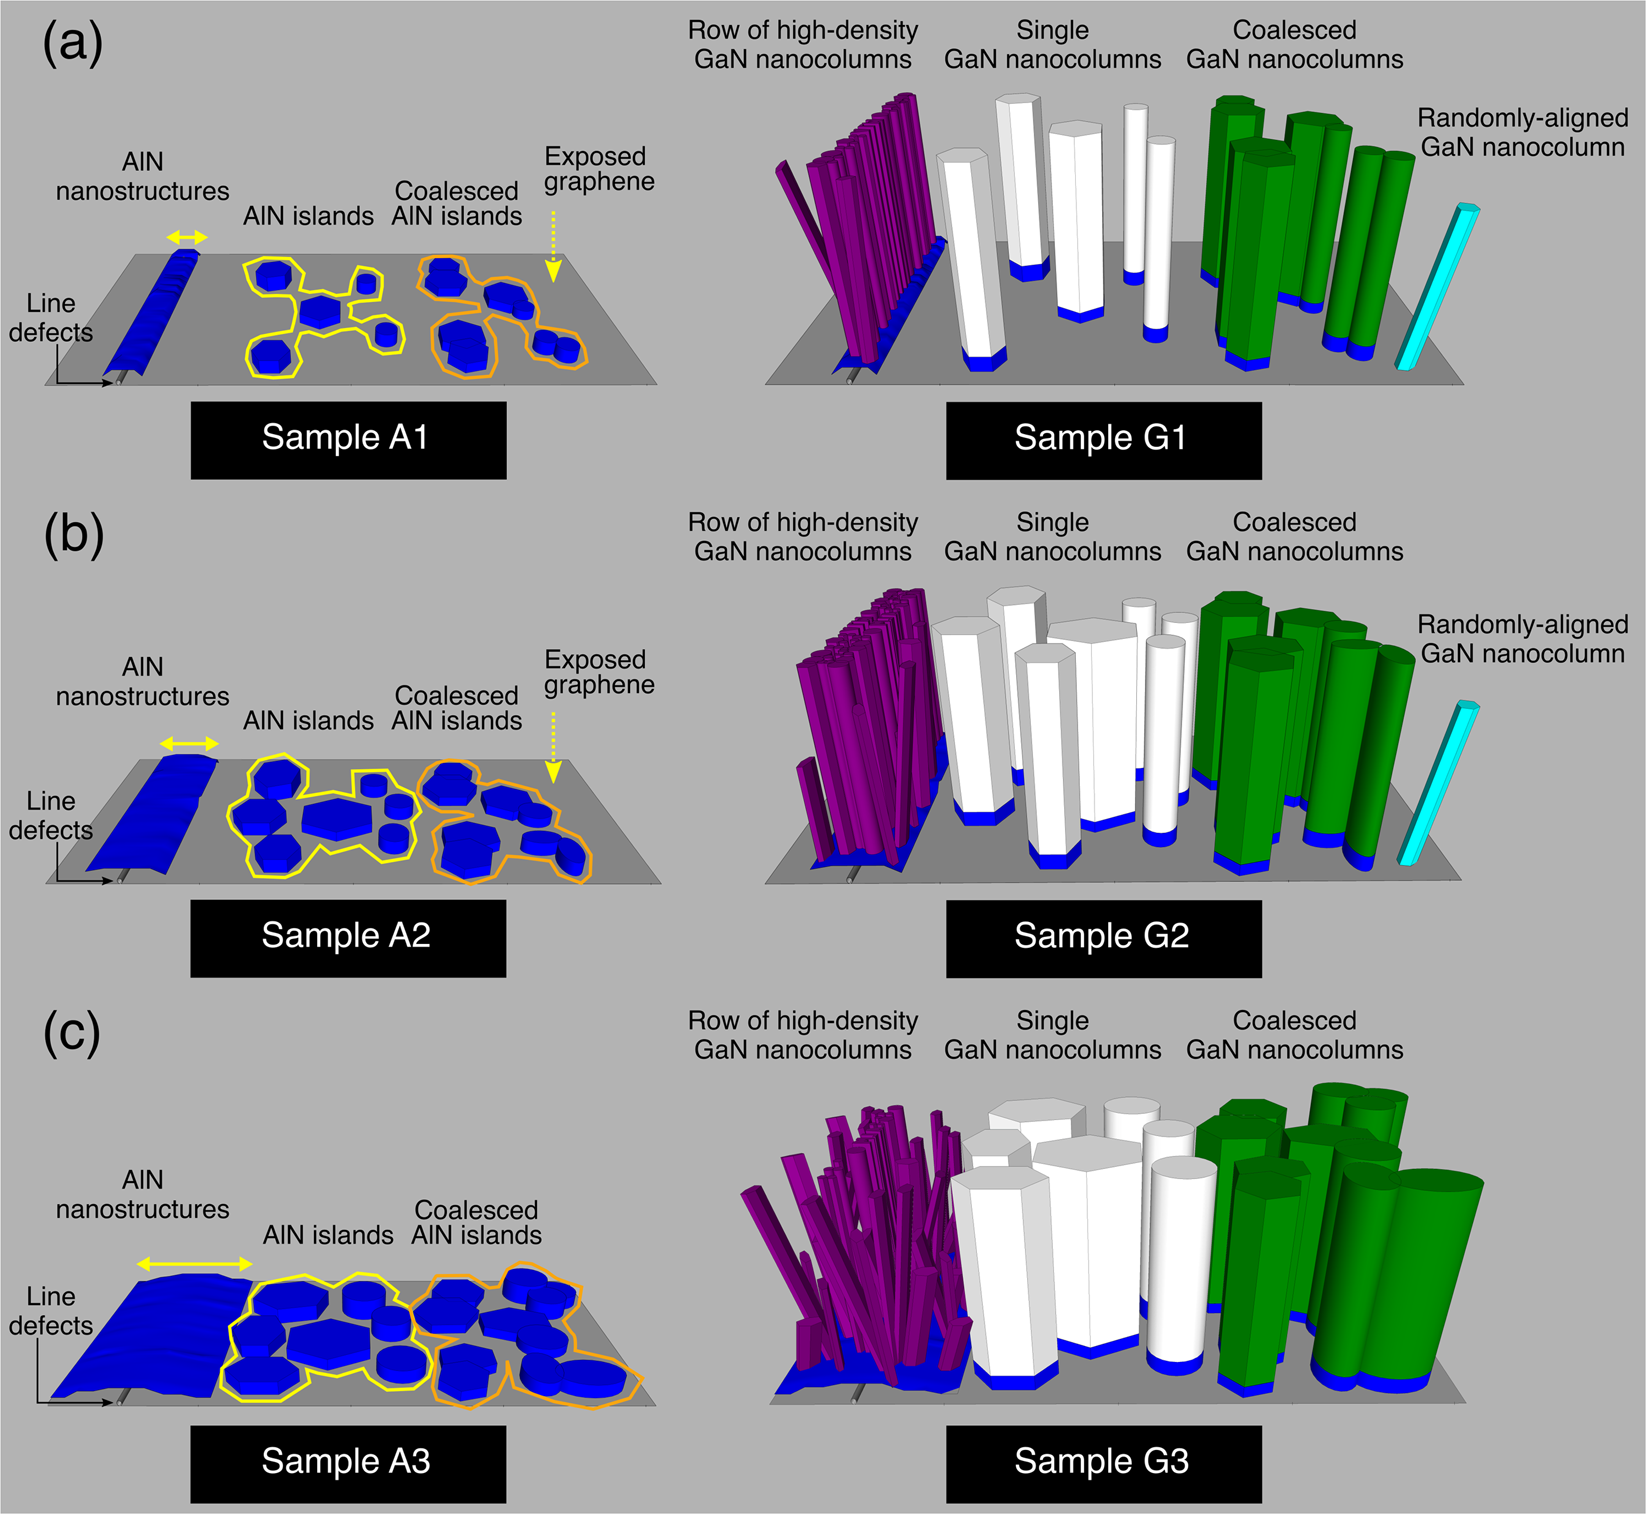
\includegraphics[width=\textwidth]{figures/paper-iv/fig-4.png}
    \caption[Simplified schematics of the AlN buffer structures and GaN nanocolumn formation on graphene]{Simplified schematics of the AlN buffer structures and GaN nanocolumn formation on graphene. Samples (\textbf{a}) A1-G1, (\textbf{b}) A2-G2 and (\textbf{c}) A3-G3. There are two possible AlN (blue) nanostructures forming on graphene: 1) AlN islands and 2) AlN nanostructures along the line defects of graphene (the yellow arrows indicate their lateral growth spread further away from the line defects). Single (white) and coalesced (green) vertical GaN nanocolumn structures are nucleated from the AlN islands, while row of high-density nanocolumns (purple) form on the AlN nanostructures that spread from the line defects. Additional tilted nanocolumns (cyan) are likely to grow on exposed graphene (adapted with permission from ref. \citenum{liudimulyo2020853} \copyright \ Liudi Mulyo \textit{et al}, 2020.}
    \label{fig:figures/paper-iv/fig-4}
\end{figure}

\section{Section 1 in chapter 4}
\lipsum[2-4]

\subsection{Subsection 4.1 of section 1 in chapter 4}
\lipsum[5-7]

\subsection{Subsection 4.2 of section 1 in chapter 4}
\lipsum[8-11]

\clearpage\phantomsection % to fix wrong hyperref to this section
\section[Long section title displayed in the table of content]{Short section title in the chapter}
\sectionmark{Even shorter title on the header}
\lipsum[11-20]

\subsection{Subsection 4.2 of section 2 in chapter 4}
\lipsum[13-14]

%=======================================================================
%%% References 

% \clearpage
\phantomsection
\specialsection % put an indent, see preamble
\headerspecialsection

{\hypersetup{urlcolor=ntnu,linkcolor=sophia} % set clickable URL title color to black, not ntnu like in the main document

\bibliographystyle{unsrtnat-mod}  % NATBIB ref style
\bibliography{references}
}
% \chapter[Title of the chapter 5 displayed \\ in the table of contents]
    {Title of the chapter 5 displayed in the page
        \chaptermark{Ch. 5 title in the header}
    }
    \chaptermark{Ch. 5 title in the header}
\label{ch:labelchapter5}

\updatemylof % to be used with "list of figure divider per chapter" (see PREAMBLE)
\updatemylot % to be used with "list of table divider per chapter" (see PREAMBLE)

\regularsection
\headerregularsection

Author 1\textsuperscript{1,\textcolor{sophia}{$\ast$}}, Author 2\textsuperscript{1,2,\textcolor{sophia}{$\ast$}}, Author 3\textsuperscript{3}, Author 4\textsuperscript{1}, Author 5\textsuperscript{1}, Author 6\textsuperscript{1}, Author 7\textsuperscript{2,4,\#} and Author 8\textsuperscript{1,\#} \hfill  \newline

\let\thefootnote\relax\footnotetext{\textsuperscript{1}Department X, University 1, City A, Country B. 
\textsuperscript{2}Department Y, University 2, City C, Country D. 
\textsuperscript{3}Institute E, City F, Country G. 
\textsuperscript{4}Research Center H, University I, City J, Country K. 
\textsuperscript{\#}e-mail: \href{mailto:author7@university2.ac.countryD}{author7@university2.ac.countryD} and \href{mailto:author8@universityI.countryK}{author8@universityI.countryK}}

\noindent First published in: \textit{Scientific Reports} \textbf{10}, 853 (2020). \hfill \break
DOI: \href{https://doi.org/10.1038/s41598-019-55424-z}{10.1038/s41598-019-55424-z} 

\begin{wrapfigure}[3]{l}{0.2\textwidth}
    
\includegraphics[width=0.2\textwidth]{figures/by.png}
\end{wrapfigure} 

\noindent \textcolor{white}{test} \newline \textbf{Open Access} This article is licensed under a Creative Commons Attribution 4.0 International License. It means that unrestricted use, sharing, adaptation, distribution, and reproduction in any medium or format are allowed, as long as the original author(s) and the source are appropriately credited, a link to the Creative Commons license is provided, and any changes made are indicated. To view a copy of this license, please visit \href{http://creativecommons.org/licenses/by/4.0/}{http://creativecommons.org/licenses/by/4.0/}. \newline

\noindent \copyright \ Liudi Mulyo \textit{et al}, 2020. \newline

\noindent \textbf{Contributions} \newline
\noindent \lipsum[2]

%%%%%%%%%%%%%%%%%%%%%%%%%%%%%%%%%%%%%%%%%%%%%%%%%%%%%%%%%%%%%%%%%%%%%%%%%%%%%%%%%%%%%%%%%%%%%%%%%%%%%%%%%%%%%%%%%%%%%%%%%%%

\tcbset{enhanced,colback=abstractback,colframe=sophia,fonttitle=\bfseries}
\begin{tcolorbox}[left=3.35cm,grow to left by=3.5cm,right=3.33cm,grow to right by=3.5cm,title={\normalfont \color{White} \small \fontfamily{bch} \selectfont \scshape Abstract}]
% https://tex.stackexchange.com/questions/232878/inserting-pictures-in-tcolorbox
% https://tex.stackexchange.com/questions/169794/outer-margin-of-tcolorbox/169877
% https://tex.stackexchange.com/questions/11484/how-to-draw-a-frame-box-around-an-arbitrary-large-piece-of-text-figures-whatever
\begin{minipage}[t]{\linewidth}
\vspace*{-29pt}
\phantomsection % to fix wrong hyperref to "Abstract" 
\section*{} % for linking from TOC (only one way)
\addcontentsline{toc}{section}{Abstract}
\begin{sloppypar}
\lipsum[1]
\end{sloppypar}

\end{minipage}

\vspace*{3.5pt}
\end{tcolorbox}

%%%%%%%%%%%%%%%%%%%%%%%%%%%%%%%%%%%%%%%%%%%%%%%%%%%%%%%%%%%%%%%%%%%%%%%%%%%%%%%%%%%%%%%%%%%%%%%%%%%%%%%%%%%%%%%%%%%%%%%%%%%

\begin{sloppypar} % to suppress overfull box

As in \Autoref{ch:labelchapter4}. Lorem \index{Lorem} ipsum dolor sit amet, consectetuer adipiscing elit \cite{LIUDIMULYO201767}. Ut purus \index{purus} elit,vestibulum ut, placerat ac, adipiscing vitae, felis \citenum{LIUDIMULYO201767}. Curabitur dictum \index{dictum} gravidamauris. Nam arcu libero, nonummy eget, consectetuer id, vulputate a, magna. Donec vehicula augue eu neque \cite{liudimulyo_2018}. Pellentesque habitant morbi tristique senectuset netus et malesuada fames ac turpis egestas \index{egestas}\citenum{liudimulyo_2018}. Mauris ut leo. Cras viverra metusrhoncus sem \cite{2019liudimulyo}. Nulla et lectus vestibulum urna fringilla ultrices. Phasellus eutellus sit amet tortor gravida placerat \citenum{2019liudimulyo}. Integer sapien est, iaculis in, pretium quis,viverra ac, nunc. Praesent eget sem vel leo ultrices bibendum \cite{liudimulyo2020853}. Aenean faucibus. Morbi dolor nulla, malesuada eu, pulvinar at (\ref{fig:figures/paper-iv/fig-5}), mollis ac, nulla. Curabitur auctorsemper nulla \citenum{liudimulyo2020853}. Donec varius orci eget risus. Duis nibh mi, congue eu, accumsaneleifend, sagittis quis, diam. Duis eget orci sit amet orci dignissim rutrum \cite{LIUDIMULYO201767,liudimulyo_2018,2019liudimulyo,liudimulyo2020853,liudimulyo_unpublished1,liudimulyo_unpublished2}. For more information, see \hyperref[appendix:B]{Appendix B}, specifically in \ref{tab:appendixB}.

\end{sloppypar}

\begin{figure} % \begin{figure} will let LaTeX decide the best figure placement for you ; \begin{figure}[H] for forcing the figure placement here ; in the bottom, \begin{figure}[!b] ; top of the page, \begin{figure}[!t]
    \centering
    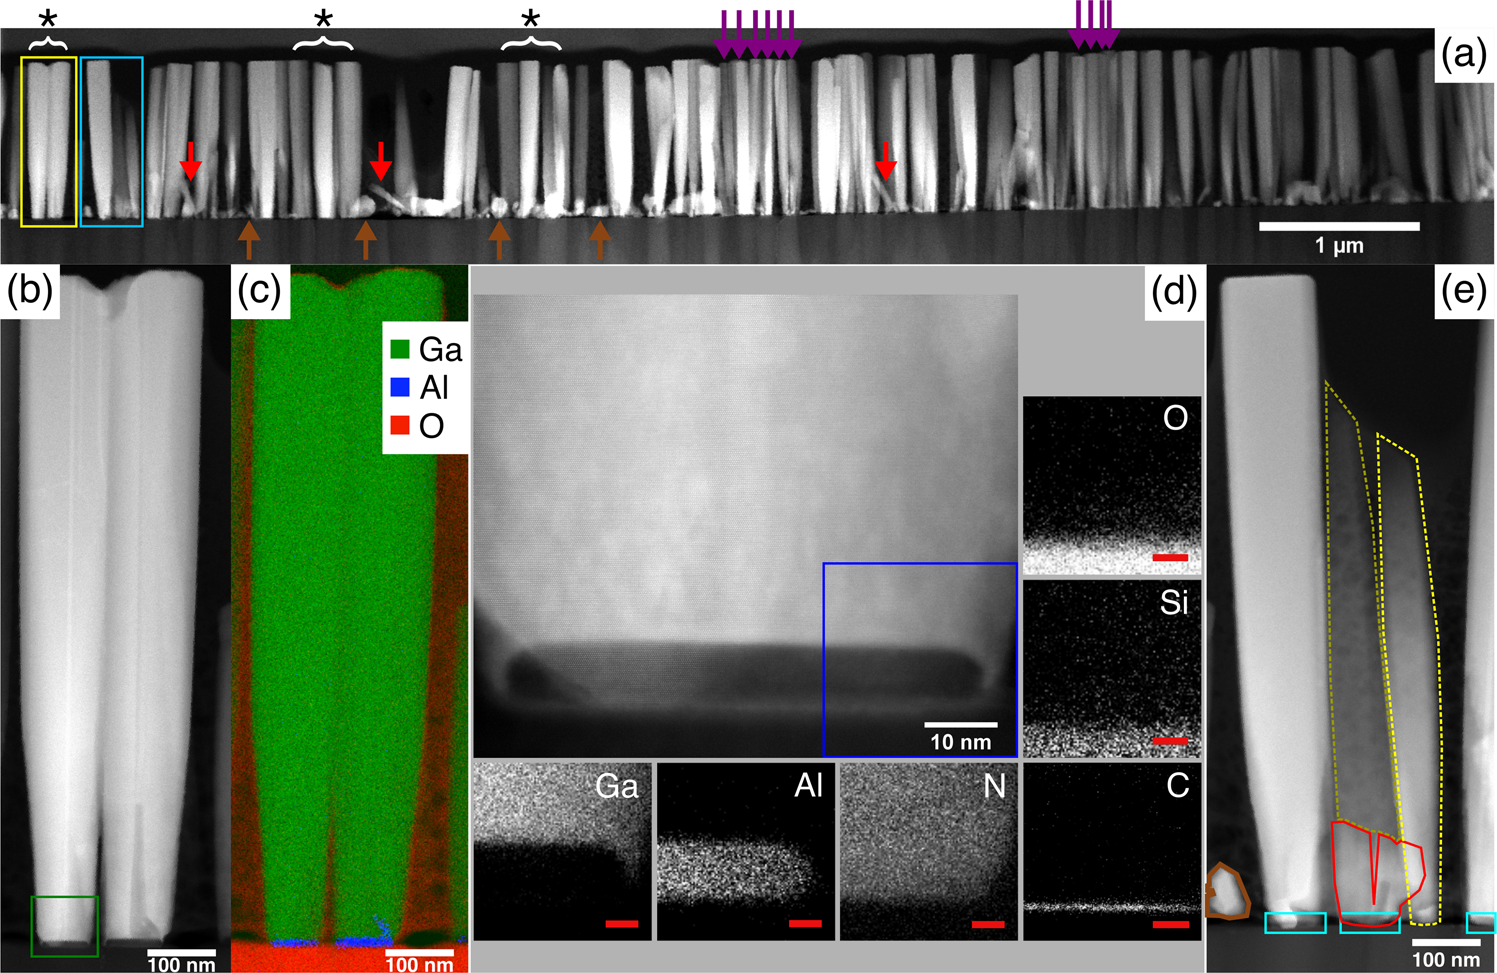
\includegraphics[width=\textwidth]{figures/paper-iv/fig-5.png}
    \caption[TEM image of GaN nanocolumn sample synthesized with\newline nominally the same growth conditions as sample G1]{TEM image of GaN nanocolumn sample synthesized with nominally the same growth conditions as sample G1. (\textbf{a}) Overview cross-sectional HAADF STEM image, showing vertical GaN nanocolumns (star-marked and purple arrows), inclined GaN nanocolumns (red arrows) and GaN crystallites (brown arrows). (\textbf{b}) HAADF STEM image of two GaN nanocolumns within yellow frame in \textbf{a}. (\textbf{c}) Combined color map of the Ga (green), Al (blue) and O (red) elemental distributions (EDS/EELS) on the corresponding region in \textbf{b}. (\textbf{d}) Magnified image of the lower part of the GaN nanocolumn near the interface of the left GaN nanocolumn in \textbf{b} (green frame), with the elemental mapping near the interfaces between the GaN nanocolumn, AlN island, graphene and silica glass (blue frame) by EDS (Ga, Al, Si) and EELS (N, O, C). The red scale bars are 5 nm. (\textbf{e}) HAADF STEM image of the GaN nanocolumns that is light-blue framed in \textbf{a}. The inclined GaN nanocolumn (yellow-dashed line) is possibly directly nucleated on graphene (indicated by the absence of any AlN layer [cyan frames] at the base). There are two broken GaN nanocolumns (red framed area) sharing the same AlN island and another inclined GaN nanocolumn (dark-yellow dashed line) in the background. An irregular GaN crystallite (brown outline) likely grown directly on graphene is also observed (adapted with permission from ref. \citenum{liudimulyo2020853} \copyright \ Liudi Mulyo \textit{et al}, 2020.}
    \label{fig:figures/paper-iv/fig-5}
\end{figure}

\section{Section 1 in chapter 5}
\lipsum[2-4]

\subsection{Subsection 5.1 of section 1 in chapter 5}
\lipsum[5-7]

\subsection{Subsection 5.2 of section 1 in chapter 5}
\lipsum[8-11]

\clearpage\phantomsection % to fix wrong hyperref to this section
\section[Long section title displayed in the table of content]{Short section title in the chapter}
\sectionmark{Even shorter title on the header}
\lipsum[11-18]
See \ref{tab:ch5}

\begin{table}[!h]
\centering
\caption{Micro-Raman peak positions, intensities and ratios}
\label{tab:ch5}
{\fontsize{7}{6}\selectfont
{\renewcommand{\arraystretch}{2}
\begin{tabular}{cccccccc}
\toprule
\multirow{3}{*}{\textbf{Sample}} & 
\multirow{3}{*}{\textbf{\begin{tabular}[c]{@{}c@{}}Median\\ D/G ratio\end{tabular}}} & 
\multicolumn{2}{c}{\textbf{Median G}} & 
\multicolumn{3}{c}{\textbf{Median 2D}} & 
\multirow{3}{*}{\textbf{\begin{tabular}[c]{@{}c@{}}Median \\ 2D/G ratio\end{tabular}}} \\
\cmidrule(l){3-4} \cmidrule(l){3-4} \cmidrule(l){3-4} \cmidrule(l){5-7} \cmidrule(l){5-7} \cmidrule(l){5-7} % repeated three times to increase the line thickness
  &  & \textbf{\begin{tabular}[c]{@{}c@{}}Position \\ {[} cm\textsuperscript{-1} {]}\end{tabular}} & \textbf{\begin{tabular}[c]{@{}c@{}}Intensity \\ {[} cps {]}\end{tabular}} & \textbf{\begin{tabular}[c]{@{}c@{}}Position \\ {[} cm\textsuperscript{-1} {]}\end{tabular}} & \textbf{\begin{tabular}[c]{@{}c@{}}Intensity \\ {[} cps {]}\end{tabular}} & \textbf{\begin{tabular}[c]{@{}c@{}}FWHM \\ {[} cm\textsuperscript{-1} {]}\end{tabular}} &  \\
\midrule
\begin{tabular}[c]{@{}c@{}}DLG before\\ MBE growth\end{tabular} & 1 & 2 & 3 & 4 & 5 & 6 & 7 \\
\rowcolor{Gray} \begin{tabular}[c]{@{}c@{}}DLG after\\ MBE growth\end{tabular} & 1 & 2 & 3 & 4 & 5 & 6 & 7 \\
\bottomrule
\end{tabular}
}
}
\end{table}

\subsection{Subsection 5.2 of section 2 in chapter 5}
\lipsum[13-14]

%=======================================================================
%%% References 

% \clearpage
\phantomsection
\specialsection % put an indent, see preamble
\headerspecialsection

{\hypersetup{urlcolor=ntnu,linkcolor=sophia} % set clickable URL title color to black, not ntnu like in the main document

\bibliographystyle{unsrtnat-mod}  % NATBIB ref style
\bibliography{references}
}
% \chapter[Title of the chapter 6 displayed \\ in the table of contents]
    {Title of the chapter 6 displayed in the page
        \chaptermark{Ch. 6 title in the header}
    }
    \chaptermark{Ch. 6 title in the header}
\label{ch:labelchapter6}

\updatemylof % to be used with "list of figure divider per chapter" (see PREAMBLE)
\updatemylot % to be used with "list of table divider per chapter" (see PREAMBLE)

\regularsection
\headerregularsection

Author 1\textsuperscript{1,\textcolor{sophia}{$\ast$}}, Author 2\textsuperscript{1,2,\textcolor{sophia}{$\ast$}}, Author 3\textsuperscript{3}, Author 4\textsuperscript{1}, Author 5\textsuperscript{1}, Author 6\textsuperscript{1}, Author 7\textsuperscript{2,4,\#} and Author 8\textsuperscript{1,\#} \hfill  \newline

\let\thefootnote\relax\footnotetext{\textsuperscript{1}Department X, University 1, City A, Country B. 
\textsuperscript{2}Department Y, University 2, City C, Country D. 
\textsuperscript{3}Institute E, City F, Country G. 
\textsuperscript{4}Research Center H, University I, City J, Country K. 
\textsuperscript{\#}e-mail: \href{mailto:author7@university2.ac.countryD}{author7@university2.ac.countryD} and \href{mailto:author8@universityI.countryK}{author8@universityI.countryK}}

\noindent First published in: \textit{Scientific Reports} \textbf{10}, 853 (2020). \hfill \break
DOI: \href{https://doi.org/10.1038/s41598-019-55424-z}{10.1038/s41598-019-55424-z} 

\begin{wrapfigure}[3]{l}{0.2\textwidth}
    
\includegraphics[width=0.2\textwidth]{figures/by.png}
\end{wrapfigure} 

\noindent \textcolor{white}{test} \newline \textbf{Open Access} This article is licensed under a Creative Commons Attribution 4.0 International License. It means that unrestricted use, sharing, adaptation, distribution, and reproduction in any medium or format are allowed, as long as the original author(s) and the source are appropriately credited, a link to the Creative Commons license is provided, and any changes made are indicated. To view a copy of this license, please visit \href{http://creativecommons.org/licenses/by/4.0/}{http://creativecommons.org/licenses/by/4.0/}. \newline

\noindent \copyright \ Liudi Mulyo \textit{et al}, 2020. \newline

\noindent \textbf{Contributions} \newline
\noindent \lipsum[2]

%%%%%%%%%%%%%%%%%%%%%%%%%%%%%%%%%%%%%%%%%%%%%%%%%%%%%%%%%%%%%%%%%%%%%%%%%%%%%%%%%%%%%%%%%%%%%%%%%%%%%%%%%%%%%%%%%%%%%%%%%%%

\tcbset{enhanced,colback=abstractback,colframe=sophia,fonttitle=\bfseries}
\begin{tcolorbox}[left=3.35cm,grow to left by=3.5cm,right=3.33cm,grow to right by=3.5cm,title={\normalfont \color{White} \small \fontfamily{bch} \selectfont \scshape Abstract}]
% https://tex.stackexchange.com/questions/232878/inserting-pictures-in-tcolorbox
% https://tex.stackexchange.com/questions/169794/outer-margin-of-tcolorbox/169877
% https://tex.stackexchange.com/questions/11484/how-to-draw-a-frame-box-around-an-arbitrary-large-piece-of-text-figures-whatever
\begin{minipage}[t]{\linewidth}
\vspace*{-29pt}
\phantomsection % to fix wrong hyperref to "Abstract" 
\section*{} % for linking from TOC (only one way)
\addcontentsline{toc}{section}{Abstract}
\begin{sloppypar}
\lipsum[1]
\end{sloppypar}

\end{minipage}

\vspace*{3.5pt}
\end{tcolorbox}

%%%%%%%%%%%%%%%%%%%%%%%%%%%%%%%%%%%%%%%%%%%%%%%%%%%%%%%%%%%%%%%%%%%%%%%%%%%%%%%%%%%%%%%%%%%%%%%%%%%%%%%%%%%%%%%%%%%%%%%%%%%

\begin{sloppypar} % to suppress overfull box

As in \Autoref{ch:labelchapter5}. Lorem \index{Lorem} ipsum dolor sit amet, consectetuer adipiscing elit \cite{LIUDIMULYO201767}. Ut purus \index{purus} elit,vestibulum ut, placerat ac, adipiscing vitae, felis \citenum{LIUDIMULYO201767}. Curabitur dictum \index{dictum} gravidamauris. Nam arcu libero, nonummy eget, consectetuer id, vulputate a, magna. Donec vehicula augue eu neque \cite{liudimulyo_2018}. Pellentesque habitant morbi tristique senectuset netus et malesuada fames ac turpis egestas \index{egestas}\citenum{liudimulyo_2018}. Mauris ut leo. Cras viverra metusrhoncus sem \cite{2019liudimulyo}. Nulla et lectus vestibulum urna fringilla ultrices. Phasellus eutellus sit amet tortor gravida placerat \citenum{2019liudimulyo}. Integer sapien est, iaculis in, pretium quis,viverra ac, nunc. Praesent eget sem vel leo ultrices bibendum \cite{liudimulyo2020853}. Aenean faucibus. Morbi dolor nulla, malesuada eu, pulvinar at (\ref{fig:figures/paper-iv/fig-6}), mollis ac, nulla. Curabitur auctorsemper nulla \citenum{liudimulyo2020853}. Donec varius orci eget risus. Duis nibh mi, congue eu, accumsaneleifend, sagittis quis, diam. Duis eget orci sit amet orci dignissim rutrum \cite{LIUDIMULYO201767,liudimulyo_2018,2019liudimulyo,liudimulyo2020853,liudimulyo_unpublished1,liudimulyo_unpublished2}.

\end{sloppypar}

\begin{figure} % \begin{figure} will let LaTeX decide the best figure placement for you ; \begin{figure}[H] for forcing the figure placement here ; in the bottom, \begin{figure}[!b] ; top of the page, \begin{figure}[!t]
    \centering
    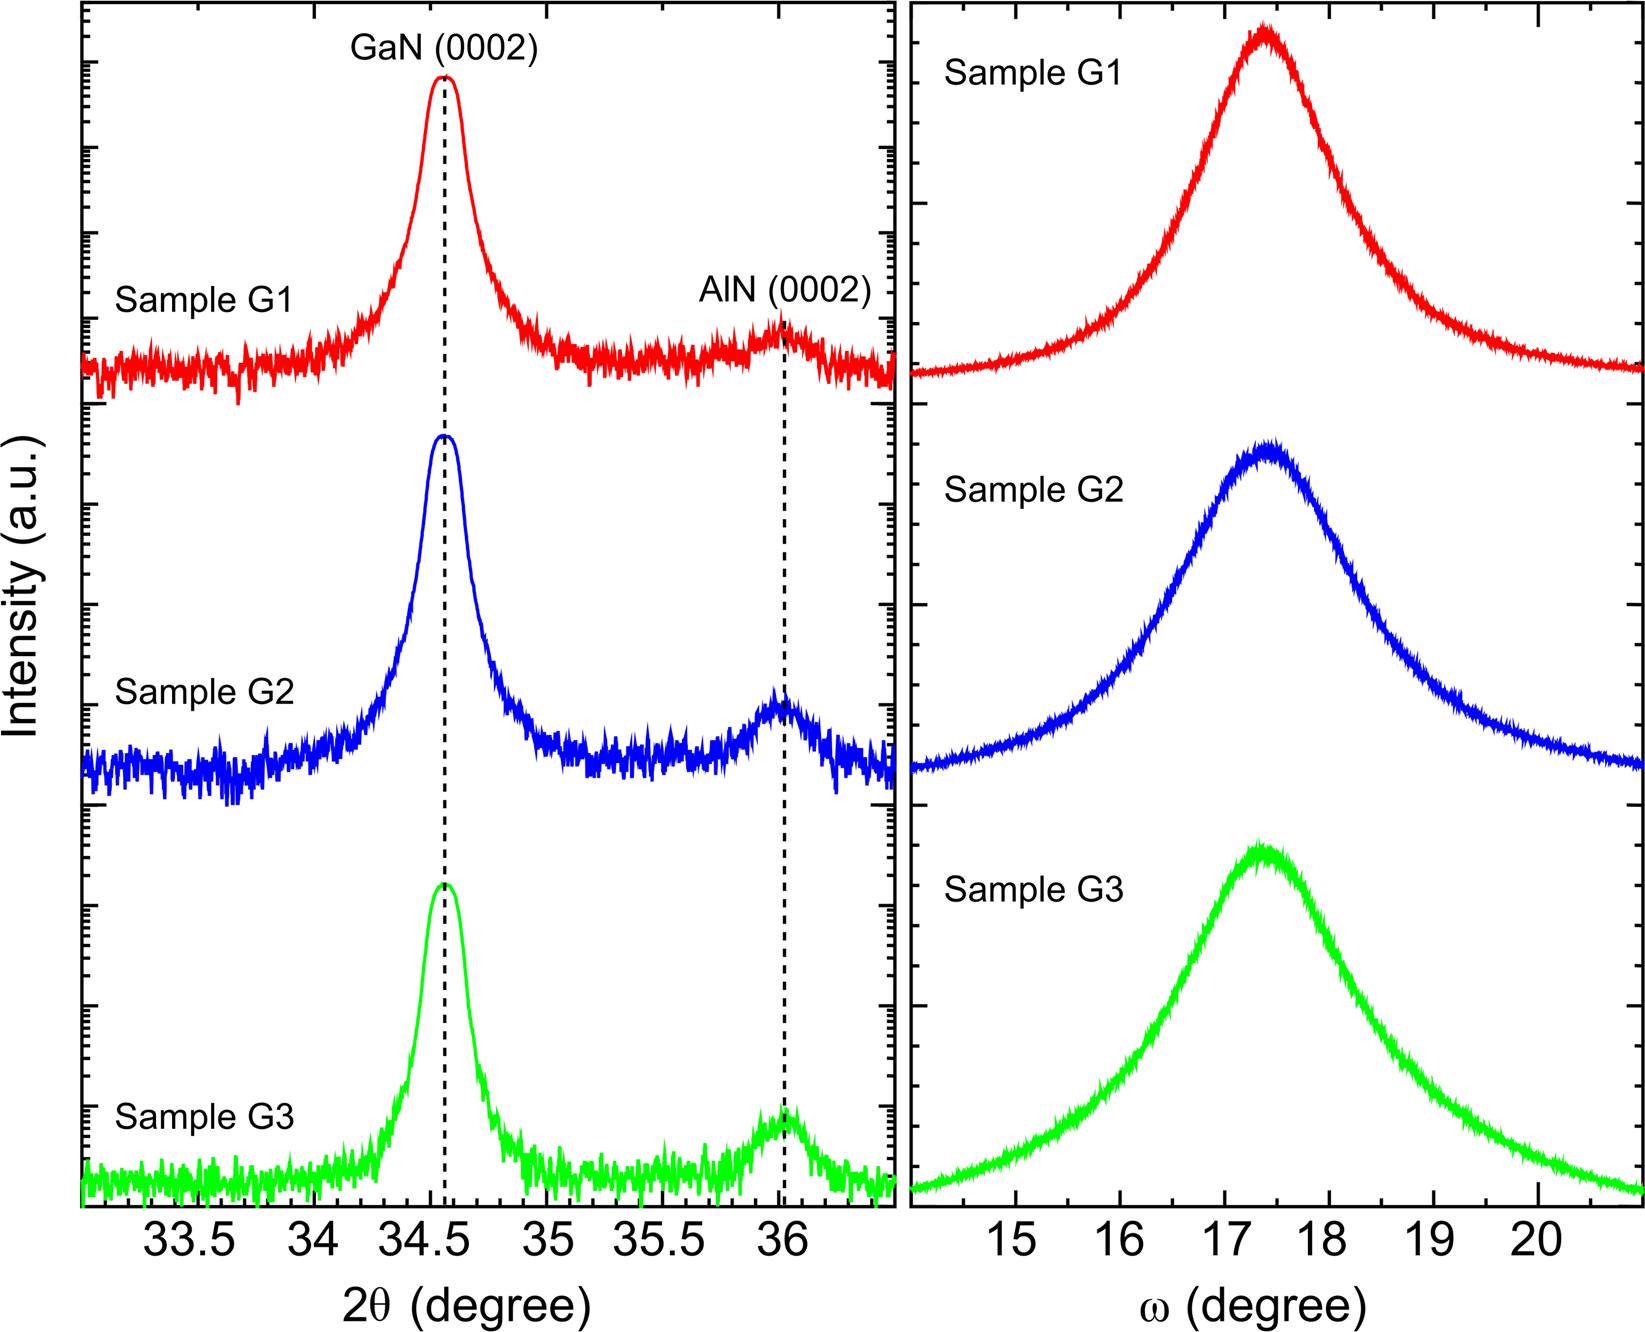
\includegraphics[width=\textwidth]{figures/paper-iv/fig-6.png}
    \caption[HRXRD measurements of the nanocolumns]{HRXRD measurements of the nanocolumns. (\textbf{a}) 2\straighttheta-\textomega \ scanning curve and (\textbf{b}) \textomega \ scanning curve of samples G1, G2 and G3 (adapted with permission from ref. \citenum{liudimulyo2020853} \copyright \ Liudi Mulyo \textit{et al}, 2020.}
    \label{fig:figures/paper-iv/fig-6}
\end{figure}

\section{Section 1 in chapter 6}
\lipsum[2-4]

\subsection{Subsection 6.1 of section 1 in chapter 6}
\lipsum[5-7]

\subsection{Subsection 6.2 of section 1 in chapter 6}
\lipsum[8-11]

\clearpage\phantomsection % to fix wrong hyperref to this section
\section[Long section title displayed in the table of content]{Short section title in the chapter}
\sectionmark{Even shorter title on the header}
\lipsum[11-18]
See \ref{tab:ch6}

\begin{table}[H]
\centering
\caption[Al-content of each axial nanocolumn segment for the vertical GaN/AlGaN nanocolumn ensemble obtained from fitting the simulation model to the HRXRD 2\straighttheta-\textomega \ scan data]{Al-content of each axial nanocolumn segment for the vertical GaN/AlGaN nanocolumn ensemble (top to bottom) obtained from fitting the simulation model to the HRXRD 2\straighttheta-\textomega \ scan data}
\label{tab:ch6}
{\fontsize{7}{6}\selectfont
{\renewcommand{\arraystretch}{2}
\begin{tabular}{cccc}
\textbf{Segment} & \textbf{Thickness (nm)} & \textbf{Al bottom (\%)} & \textbf{Al top (\%)} \\
\midrule
\begin{tabular}[c]{@{}c@{}}\textit{p-}GaN\end{tabular} & 1 & 2 & 3 \\
\rowcolor{Gray}\begin{tabular}[c]{@{}c@{}}\textit{p-}AlGaN (linear grading)\end{tabular} & 4 & 5 & 6 \\
\begin{tabular}[c]{@{}c@{}}\textit{i-}GaN quantum disk\end{tabular} & 7 & 8 & 9 \\
\rowcolor{Gray}\begin{tabular}[c]{@{}c@{}}\textit{n-}AlGaN (linear grading)\end{tabular} & 10 & 11 & 12 \\
\begin{tabular}[c]{@{}c@{}}\textit{n-}GaN\end{tabular} & 13 & 14 & 15 \\
\rowcolor{Gray}\begin{tabular}[c]{@{}c@{}}\textit{n-}AlN buffer layer\end{tabular} & 16 & 17 & 18 \\
\end{tabular}
}
}
\end{table}

\subsection{Subsection 6.2 of section 2 in chapter 6}
\label{subsec:labelsubsec6-2}
\lipsum[13-14]
See \hyperref[appendix:C]{Appendix C} for the \ref{fig:figures/paper-iv/fig-7} and \ref{fig:figures/paper-iv/fig-8}.

%=======================================================================
%%% References 

% \clearpage
\phantomsection
\specialsection % put an indent, see preamble
\headerspecialsection

{\hypersetup{urlcolor=ntnu,linkcolor=sophia} % set clickable URL title color to black, not ntnu like in the main document

\bibliographystyle{unsrtnat-mod}  % NATBIB ref style
\bibliography{references}
}

\cleardoublepage\phantomsection % to fix wrong hyperref to \part{Epilogue}
\part{Epilogue}

%\chapter[Conclusion]{Conclusion}
\markboth{Chap. 7\ \ \enspace Conclusion}{Chap 7. Conclusion}

\regularsection
\headerregularsection

\begin{sloppypar} % to suppress overfull box

Lorem \index{Lorem} ipsum dolor sit amet, consectetuer adipiscing elit \cite{LIUDIMULYO201767}. Ut purus \index{purus} elit,vestibulum ut, placerat ac, adipiscing vitae, felis \citenum{LIUDIMULYO201767}. Curabitur dictum \index{dictum} gravidamauris. Nam arcu libero, nonummy eget, consectetuer id, vulputate a, magna. Donec vehicula augue eu neque \cite{liudimulyo_2018}. Pellentesque habitant morbi tristique senectuset netus et malesuada fames ac turpis egestas \index{egestas}\citenum{liudimulyo_2018}. Mauris ut leo. Cras viverra metusrhoncus sem \cite{2019liudimulyo}. Nulla et lectus vestibulum urna fringilla ultrices. Phasellus eutellus sit amet tortor gravida placerat \citenum{2019liudimulyo}. Integer sapien est, iaculis in, pretium quis,viverra ac, nunc. Praesent eget sem vel leo ultrices bibendum \cite{liudimulyo2020853}. Aenean faucibus. Morbi dolor nulla, malesuada eu, pulvinar at (\ref{fig:figures/paper-iv/fig-1}), mollis ac, nulla. Curabitur auctorsemper nulla \citenum{liudimulyo2020853}. Donec varius orci eget risus. Duis nibh mi, congue eu, accumsaneleifend, sagittis quis, diam. Duis eget orci sit amet orci dignissim rutrum \cite{LIUDIMULYO201767,liudimulyo_2018,2019liudimulyo,liudimulyo2020853,liudimulyo_unpublished1,liudimulyo_unpublished2}. For \Autoref{ch:labelchapter4} and \Autoref{ch:labelchapter5}, as well as \Autoref{ch:labelchapter6}

\end{sloppypar}

\section{Section 1 in chapter 7}
\lipsum[2-4]

\subsection{Subsection 7.1 of section 1 in chapter 7}
\lipsum[5-7]

\subsection{Subsection 7.2 of section 1 in chapter 7}
\lipsum[8-11]

\clearpage\phantomsection % to fix wrong hyperref to this section
\section[Long section title displayed in the table of content]{Short section title in the chapter}
\sectionmark{Even shorter title on the header}
\lipsum[11-19]

\subsection{Subsection 7.2 of section 2 in chapter 7}
\lipsum[13-14]

%=======================================================================
%%% References 

% \clearpage
\phantomsection
\specialsection % put an indent, see preamble
\headerspecialsection

{\hypersetup{urlcolor=ntnu,linkcolor=sophia} % set clickable URL title color to black, not ntnu like in the main document

\bibliographystyle{unsrtnat-mod}  % NATBIB ref style
\bibliography{references}
}

%=======================================================================

\vspace{2.81ex}

\begin{center}
    {\color{sophia} \Huge
    \adforn{21}
    }
\end{center}

\clearpage\null\thispagestyle{empty}

%=======================================================================

%%% Back matter
\backmatter

%%%% Appendix A

\chapter[Appendix A \hspace{0.0025em} Supplementary information for chapter 4]{\textsc{Appendix A} \vspace{8pt} \\ Supporting information for chapter 4}

\label{appendix:A}

\setcounter{page}{1}
\renewcommand{\thepage}{A-\arabic{page}}

\setcounter{chapter}{0}
\renewcommand{\thechapter}{\Alph{chapter}}
\renewcommand{\theHchapter}{A\thechapter}

\setcounter{section}{0}
\renewcommand{\thesection}{A.\arabic{section}}

\setcounter{figure}{0}
\renewcommand{\thefigure}{A.\arabic{figure}}

\setcounter{table}{0}
\renewcommand{\thetable}{A.\arabic{table}}

% \updatemylofappendixA % uncomment this if this appendix has figure -> ToC will be updated
\updatemylotappendixA

\markboth{Appendix A \hspace{0.0025em} Supplementary information for chapter 4}
{Appendix A \hspace{0.0025em} Supplementary information for chapter 4}

\regularsection
\headerspecialsectionappendix

% ============================================================================================================

\section{Detailed growth information}

\begin{sloppypar} % to suppress overfull box

Lorem \index{Lorem} ipsum dolor sit amet, consectetuer adipiscing elit \cite{LIUDIMULYO201767}. Ut purus \index{purus} elit,vestibulum ut, placerat ac, adipiscing vitae, felis \citenum{LIUDIMULYO201767}. Curabitur dictum \index{dictum} gravidamauris. Nam arcu libero, nonummy eget, consectetuer id, vulputate a, magna. Donec vehicula augue eu neque \cite{liudimulyo_2018}. Pellentesque habitant morbi tristique senectuset netus et malesuada fames ac turpis egestas \index{egestas}\citenum{liudimulyo_2018}. Mauris ut leo. Cras viverra metusrhoncus sem \cite{2019liudimulyo}. Nulla et lectus vestibulum urna fringilla ultrices. Phasellus eutellus sit amet tortor gravida placerat \citenum{2019liudimulyo}. Integer sapien est, iaculis in, pretium quis,viverra ac, nunc. Praesent eget sem vel leo ultrices bibendum \cite{liudimulyo2020853}. Aenean faucibus. Morbi dolor nulla, malesuada eu, pulvinar at (\ref{fig:figures/paper-iv/fig-4}), mollis ac, nulla. Curabitur auctorsemper nulla \citenum{liudimulyo2020853}. Donec varius orci eget risus. Duis nibh mi, congue eu, accumsaneleifend, sagittis quis, diam. Duis eget orci sit amet orci dignissim rutrum \cite{LIUDIMULYO201767,liudimulyo_2018,2019liudimulyo,liudimulyo2020853,liudimulyo_unpublished1,liudimulyo_unpublished2}.

\end{sloppypar}

\begin{table}[!h]
\centering
\caption{Detailed growth conditions of nanocolumns} % use this to compensate "from tcbcaption to break the long sentence" in PREAMBLE instead if the "default" one
\label{tab:appendixA}
\rotatebox{90}{
\begin{minipage}{17cm}
\centering
{\renewcommand{\arraystretch}{1.5}
\begin{tabular}{cccccccc}
\toprule
\multirow{3}{*}{\textbf{\begin{tabular}[c]{@{}c@{}} Nanocolumn\\ segment/layer \\\end{tabular}}} & \multirow{2}{*}{\textbf{\begin{tabular}[c]{@{}c@{}} Growth temperature, \\ pyrometer reading \\ ($^\circ$C)\end{tabular}}} & 
\multicolumn{3}{c}{\textbf{\begin{tabular}[c]{@{}c@{}} Beam equivalent pressure (Pa)\end{tabular}}} & \multirow{2}{*}{\textbf{\begin{tabular}[c]{@{}c@{}}Si cell\\ temperature\\ ($^\circ$C)\end{tabular}}} & \multirow{2}{*}{\textbf{\begin{tabular}[c]{@{}c@{}}N\textsubscript{2} flow rate/ \\ plasma emission\\  (sccm/mV)\end{tabular}}} & 
\multirow{3}{*}{\textbf{\begin{tabular}[c]{@{}c@{}} Growth time\\ (sec)\end{tabular}}} \\
\cmidrule(l){3-5} \cmidrule(l){3-5} \cmidrule(l){3-5} % repeated three times to increase the line thickness
 &  & \multirow{2}{*}{\textbf{\begin{tabular}[c]{@{}c@{}}Al\end{tabular}}} & \multirow{2}{*}{\textbf{\begin{tabular}[c]{@{}c@{}}Ga\end{tabular}}} & \multirow{2}{*}{\textbf{\begin{tabular}[c]{@{}c@{}}Mg\end{tabular}}} &  &  &  \\
\multicolumn{1}{l}{} & \multicolumn{1}{l}{} & \multicolumn{1}{l}{} & \multicolumn{1}{l}{} & \multicolumn{1}{l}{} & \multicolumn{1}{l}{} & \multicolumn{1}{l}{} & \multicolumn{1}{l}{} \\
\midrule
\begin{tabular}[c]{@{}c@{}} 
Al seeding\\ with Si\end{tabular} & 1 & 2.0 $\times$ 10\textsuperscript{-3} & - & - & 4 & - & 5 \\

\cellcolor{Gray} & \cellcolor{Gray} & \cellcolor{Gray} & \cellcolor{Gray} & \cellcolor{Gray} & \cellcolor{Gray} & \cellcolor{Gray} & \cellcolor{Gray} \\
\multirow{-2}{*}{\cellcolor{Gray} Nitridation} & \multirow{-2}{*}{\cellcolor{Gray} 6} & \multirow{-2}{*}{\cellcolor{Gray} -} & \multirow{-2}{*}{\cellcolor{Gray} -} & \multirow{-2}{*}{\cellcolor{Gray} -} & \multirow{-2}{*}{\cellcolor{Gray} -} & \multirow{-2}{*}{\cellcolor{Gray} 7.00/8.9} & \multirow{-2}{*}{\cellcolor{Gray} 1} \\

\cellcolor{White} & \cellcolor{White} & \cellcolor{White} & \cellcolor{White} & \cellcolor{White} & \cellcolor{White} & \cellcolor{White} & \cellcolor{White} \\
\multirow{-2}{*}{\cellcolor{White} n-AlN} & \multirow{-2}{*}{\cellcolor{White} 2} & \multirow{-2}{*}{\cellcolor{White} 3.0 $\times$ 10\textsuperscript{-4}} & \multirow{-2}{*}{\cellcolor{White} -} & \multirow{-2}{*}{\cellcolor{White} -} & \multirow{-2}{*}{\cellcolor{White} 5} & \multirow{-2}{*}{\cellcolor{White} 6.00/7.89} & \multirow{-2}{*}{\cellcolor{White} 1} \\

\cellcolor{Gray} & \cellcolor{Gray} & \cellcolor{Gray} & \cellcolor{Gray} & \cellcolor{Gray} & \cellcolor{Gray} & \cellcolor{Gray} & \cellcolor{Gray} \\
\multirow{-2}{*}{\cellcolor{Gray} n-GaN} & \multirow{-2}{*}{\cellcolor{Gray} 2} & \multirow{-2}{*}{\cellcolor{Gray} -} & \multirow{-2}{*}{\cellcolor{Gray} 3.4 $\times$ 10\textsuperscript{-5}} & \multirow{-2}{*}{\cellcolor{Gray} -} & \multirow{-2}{*}{\cellcolor{Gray} 6} & \multirow{-2}{*}{\cellcolor{Gray} 7.89/1.23} & \multirow{-2}{*}{\cellcolor{Gray} 4} \\

\cellcolor{White} & \cellcolor{White} & \cellcolor{White} & \cellcolor{White} & \cellcolor{White} & \cellcolor{White} & \cellcolor{White} & \cellcolor{White} \\
\multirow{-2}{*}{\cellcolor{White} n-Al\textsubscript{0.56}Ga\textsubscript{0.78}N} & \multirow{-2}{*}{\cellcolor{White} 9} & \multirow{-2}{*}{\cellcolor{White} 1.2 $\times$ 10\textsuperscript{-3}} & \multirow{-2}{*}{\cellcolor{White} 4.0 $\times$ 10\textsuperscript{-5}} & \multirow{-2}{*}{\cellcolor{White} -} & \multirow{-2}{*}{\cellcolor{White} 6} & \multirow{-2}{*}{\cellcolor{White} 7.00/8.9} & \multirow{-2}{*}{\cellcolor{White} 1} \\

\cellcolor{Gray} & \cellcolor{Gray} & \cellcolor{Gray} & \cellcolor{Gray} & \cellcolor{Gray} & \cellcolor{Gray} & \cellcolor{Gray} & \cellcolor{Gray} \\
\multirow{-2}{*}{\cellcolor{Gray} i-GaN} & \multirow{-2}{*}{\cellcolor{Gray} 2} & \multirow{-2}{*}{\cellcolor{Gray} -} & \multirow{-2}{*}{\cellcolor{Gray} 3.1 $\times$ 10\textsuperscript{-2}} & \multirow{-2}{*}{\cellcolor{Gray} -} & \multirow{-2}{*}{\cellcolor{Gray} -} & \multirow{-2}{*}{\cellcolor{Gray} 3.45/6.78} & \multirow{-2}{*}{\cellcolor{Gray} 9} \\

\cellcolor{White} & \cellcolor{White} & \cellcolor{White} & \cellcolor{White} & \cellcolor{White} & \cellcolor{White} & \cellcolor{White} & \cellcolor{White} \\
\multirow{-2}{*}{\cellcolor{White} p-Al\textsubscript{1.23}Ga\textsubscript{4.56}N} & \multirow{-2}{*}{\cellcolor{White} 7} & \multirow{-2}{*}{\cellcolor{White} 8.9 $\times$ 10\textsuperscript{-1}} & \multirow{-2}{*}{\cellcolor{White} 2.0 $\times$ 10\textsuperscript{-3}} & \multirow{-2}{*}{\cellcolor{White} 4.0 $\times$ 10\textsuperscript{-5}} & \multirow{-2}{*}{\cellcolor{White} -} & \multirow{-2}{*}{\cellcolor{White} 6.00/7.89} & \multirow{-2}{*}{\cellcolor{White} 1} \\

\cellcolor{Gray} & \cellcolor{Gray} & \cellcolor{Gray} & \cellcolor{Gray} & \cellcolor{Gray} & \cellcolor{Gray} & \cellcolor{Gray} & \cellcolor{Gray} \\
\multirow{-2}{*}{\cellcolor{Gray} p-GaN} & \multirow{-2}{*}{\cellcolor{Gray} 2} & \multirow{-2}{*}{\cellcolor{Gray} -} & \multirow{-2}{*}{\cellcolor{Gray} 3.0 $\times$ 10\textsuperscript{-4}} & \multirow{-2}{*}{\cellcolor{Gray} 5.0 $\times$ 10\textsuperscript{-6}} & \multirow{-2}{*}{\cellcolor{Gray} -} & \multirow{-2}{*}{\cellcolor{Gray} 7.00/8.9} & \multirow{-2}{*}{\cellcolor{Gray} 1} \\
\bottomrule
\end{tabular}
}
\end{minipage}
}
\end{table}

%=======================================================================
%%% References 

\clearpage
\phantomsection
\specialsection
\headerspecialsection

{\hypersetup{urlcolor=ntnu,linkcolor=sophia} % set clickable URL title color to black, not blue like in the main document

\bibliographystyle{unsrtnat-mod} % NATBIB ref style
\bibliography{references}
}

%=======================================================================
%%%% Appendix B

\chapter[Appendix B \hspace{0.0025em} Supplementary information for chapter 5]{\textsc{Appendix B} \vspace{8pt} \\ Supporting information for chapter 5}

\label{appendix:B}

\setcounter{chapter}{0}
\renewcommand{\thechapter}{\Alph{chapter}}
\renewcommand{\theHchapter}{B\thechapter}

\setcounter{section}{0}
\renewcommand{\thesection}{B.\arabic{section}}

\setcounter{figure}{0}
\renewcommand{\thefigure}{B.\arabic{figure}}

\setcounter{table}{0}
\renewcommand{\thetable}{B.\arabic{table}}

% \updatemylofappendixB % uncomment this if this appendix has figure -> ToC will be updated
\updatemylotappendixB

\markboth{Appendix B \hspace{0.0025em} Supplementary information for chapter 5}
{Appendix B \hspace{0.0025em} Supplementary information for chapter 5}

\regularsection
\headerspecialsectionappendix

% ============================================================================================================

\section{Additional micro-Raman spectroscopy measurements}

\begin{sloppypar} % to suppress overfull box

Lorem \index{Lorem} ipsum dolor sit amet, consectetuer adipiscing elit \cite{LIUDIMULYO201767}. Ut purus \index{purus} elit,vestibulum ut, placerat ac, adipiscing vitae, felis \citenum{LIUDIMULYO201767}. Curabitur dictum \index{dictum} gravidamauris. Nam arcu libero, nonummy eget, consectetuer id, vulputate a, magna. Donec vehicula augue eu neque \cite{liudimulyo_2018}. Pellentesque habitant morbi tristique senectuset netus et malesuada fames ac turpis egestas \index{egestas}\citenum{liudimulyo_2018}. Mauris ut leo. Cras viverra metusrhoncus sem \cite{2019liudimulyo}. Nulla et lectus vestibulum urna fringilla ultrices. Phasellus eutellus sit amet tortor gravida placerat \citenum{2019liudimulyo}. Integer sapien est, iaculis in, pretium quis,viverra ac, nunc. Praesent eget sem vel leo ultrices bibendum \cite{liudimulyo2020853}. Aenean faucibus. Morbi dolor nulla, malesuada eu, pulvinar at (\ref{fig:figures/paper-iv/fig-5}), mollis ac, nulla. Curabitur auctorsemper nulla \citenum{liudimulyo2020853}. Donec varius orci eget risus. Duis nibh mi, congue eu, accumsaneleifend, sagittis quis, diam. Duis eget orci sit amet orci dignissim rutrum \cite{LIUDIMULYO201767,liudimulyo_2018,2019liudimulyo,liudimulyo2020853,liudimulyo_unpublished1,liudimulyo_unpublished2}.

\end{sloppypar}

\begin{table}[!h]
\centering
\caption[Summary of micro-Raman spectroscopy measurements for the as-grown nanocolumn sample]{Summary of micro-Raman spectroscopy measurements for the as-grown nanocolumn sample carried out in different areas (of the same sample) from what is presented in \ref{fig:figures/paper-iv/fig-8}. The table shows the median values of the D peak, G peak, and 2D peak, for the entire mapping (123 measurements), from the green patches (45 measurements), and from the purple areas (67 measurements).}
\label{tab:appendixB}
{\fontsize{7}{6}\selectfont
{\renewcommand{\arraystretch}{2}
\begin{tabular}{cccccc}
\toprule
\multirow{2}{*}{\textbf{\begin{tabular}[c]{@{}c@{}}Median\\ value\end{tabular}}} & 
\multirow{2}{*}{\textbf{\begin{tabular}[c]{@{}c@{}}Area (number of\\ measurements)\end{tabular}}} & 
\multirow{2}{*}{\textbf{\begin{tabular}[c]{@{}c@{}}Position\\ {[} cm\textsuperscript{-1} {]}\end{tabular}}} & 
\multirow{2}{*}{\textbf{\begin{tabular}[c]{@{}c@{}}Intensity\\ {[} cps {]}\end{tabular}}} & 
\multirow{2}{*}{\textbf{\begin{tabular}[c]{@{}c@{}}FWHM\\ {[} cm\textsuperscript{-1} {]}\end{tabular}}} & 
\multirow{2}{*}{\textbf{\begin{tabular}[c]{@{}c@{}}Intensity ratio\\ to G peak\end{tabular}}}
\\
\\
\midrule

\multirow{3}{*}{\textbf{D peak}} & Green patches (45) & 1 & 2 & 3 & 4 \\
 & Full map (123) & 5 & 6 & 7 & 8 \\
 & Purple areas (67) & 9 & 1 & 2 & 3 \\

\cellcolor{Gray} & {\cellcolor{Gray}Green patches (45)} & {\cellcolor{Gray}4} & {\cellcolor{Gray}5} & {\cellcolor{Gray}-} & {\cellcolor{Gray}-} \\
\cellcolor{Gray} & {\cellcolor{Gray}Full map (123)} & {\cellcolor{Gray}6} & {\cellcolor{Gray}7} & {\cellcolor{Gray}-} & {\cellcolor{Gray}-} \\
\multirow{-3}{*}{\cellcolor{Gray}\textbf{G peak (*)}} & {\cellcolor{Gray}Purple areas (67)} & {\cellcolor{Gray}8} & {\cellcolor{Gray}9} & {\cellcolor{Gray}-} & {\cellcolor{Gray}-} \\

\multirow{3}{*}{\textbf{2D peak}} & Green patches (45) & 1 & 2 & 3 & 4 \\
 & Full map (123) & 5 & 6 & 7 & 8 \\
 & Purple areas (67) & 9 & 1 & 2 & 3 \\

\rowcolor{Gray}\textbf{D' peak (**)} & Green patches (45) & 4 & 5 & - & 6 \\ 

\bottomrule

\end{tabular}
}
}
\end{table}

%=======================================================================
%%% References 

\clearpage
\phantomsection
\specialsection
\headerspecialsection

{\hypersetup{urlcolor=ntnu,linkcolor=sophia} % set clickable URL title color to black, not blue like in the main document

\bibliographystyle{unsrtnat-mod} % NATBIB ref style
\bibliography{references}
}

%=======================================================================
%%%% Appendix C

\chapter[Appendix C \hspace{0.0025em} Supplementary information for chapter 6]{\textsc{Appendix C} \vspace{8pt} \\ Supplementary information for chapter 6}

\label{appendix:C}

\setcounter{chapter}{0}
\renewcommand{\thechapter}{\Alph{chapter}}
\renewcommand{\theHchapter}{C\thechapter}

\setcounter{section}{0}
\renewcommand{\thesection}{C.\arabic{section}}

\setcounter{figure}{0}
\renewcommand{\thefigure}{C.\arabic{figure}}

\setcounter{table}{0}
\renewcommand{\thetable}{C.\arabic{table}}

\updatemylofappendixC
% \updatemylotappendixC % uncomment this if this appendix has table -> ToC will be updated

\markboth{Appendix C \hspace{0.0025em} Supplementary information for chapter 6}%
{Appendix C \hspace{0.0025em} Supplementary information for chapter 6}

\regularsection
\headerspecialsectionappendix

% ============================================================================================================

\section[micro-PL spectra]{micro-photoluminescence spectra of HVPE-GaN and nanocolumn samples}

This is an additional characterization from \Autoref{subsec:labelsubsec6-2}.

\begin{figure}[H]
    \centering
    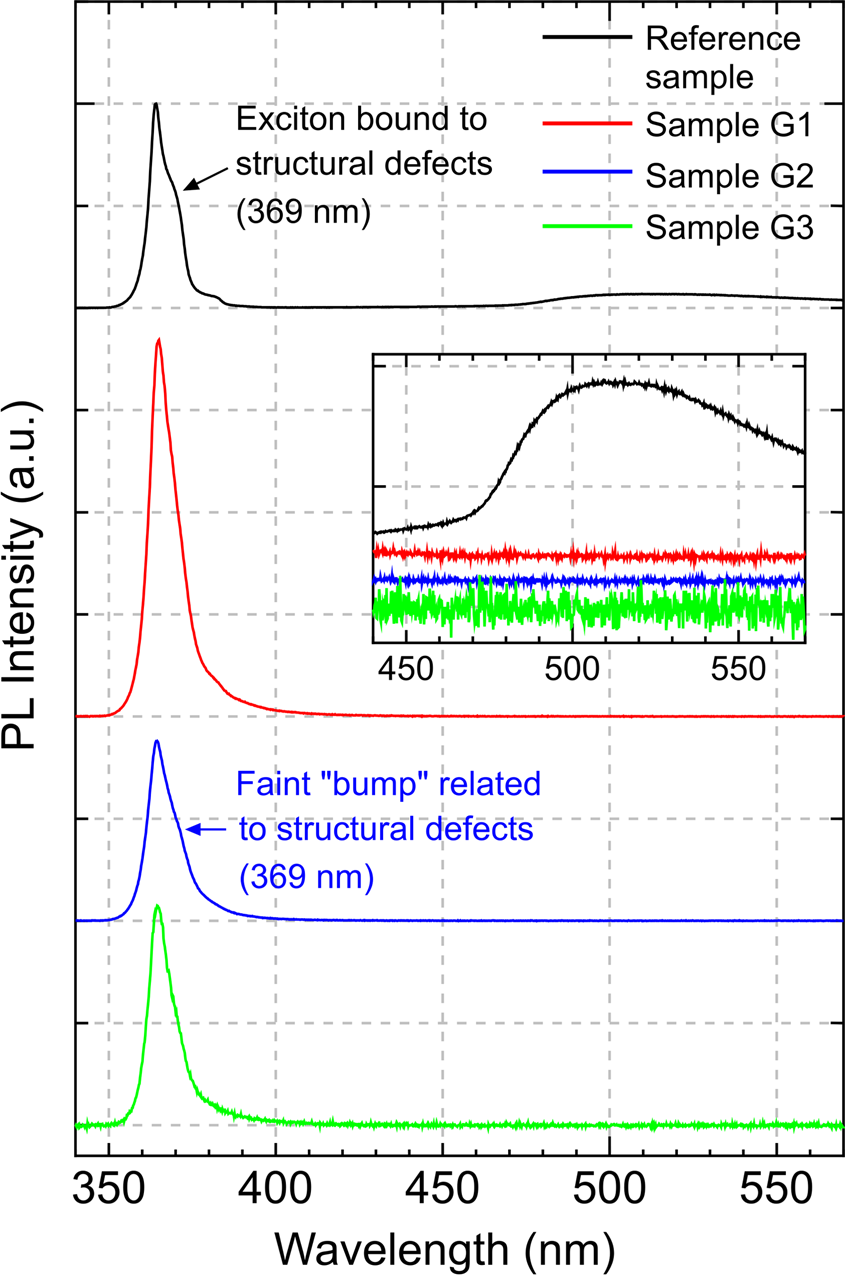
\includegraphics[width=0.6\textwidth]{figures/paper-iv/fig-7.png}
    \caption[RT micro-photoluminescence spectra of reference sample\newline (HVPE-freestanding GaN), samples G1, G2 and G3]{RT micro-photoluminescence spectra of reference sample (HVPE-freestanding GaN), samples G1, G2 and G3. Inset shows the magnified spectra in the wavelength range from 440 to 570 nm, highlighting the presence of broad green and yellow emission band in the reference sample (adapted with permission from ref. \citenum{liudimulyo2020853} \copyright \ Liudi Mulyo \textit{et al}, 2020.}
    \label{fig:figures/paper-iv/fig-7}
\end{figure}

\newpage

\section[micro-Raman spectra]{micro-Raman spectra of pristine graphene and nanocolumn samples after growth}

This is an extra measurement from \autoref{subsec:labelsubsec6-2}

\begin{figure}[H]
    \centering
    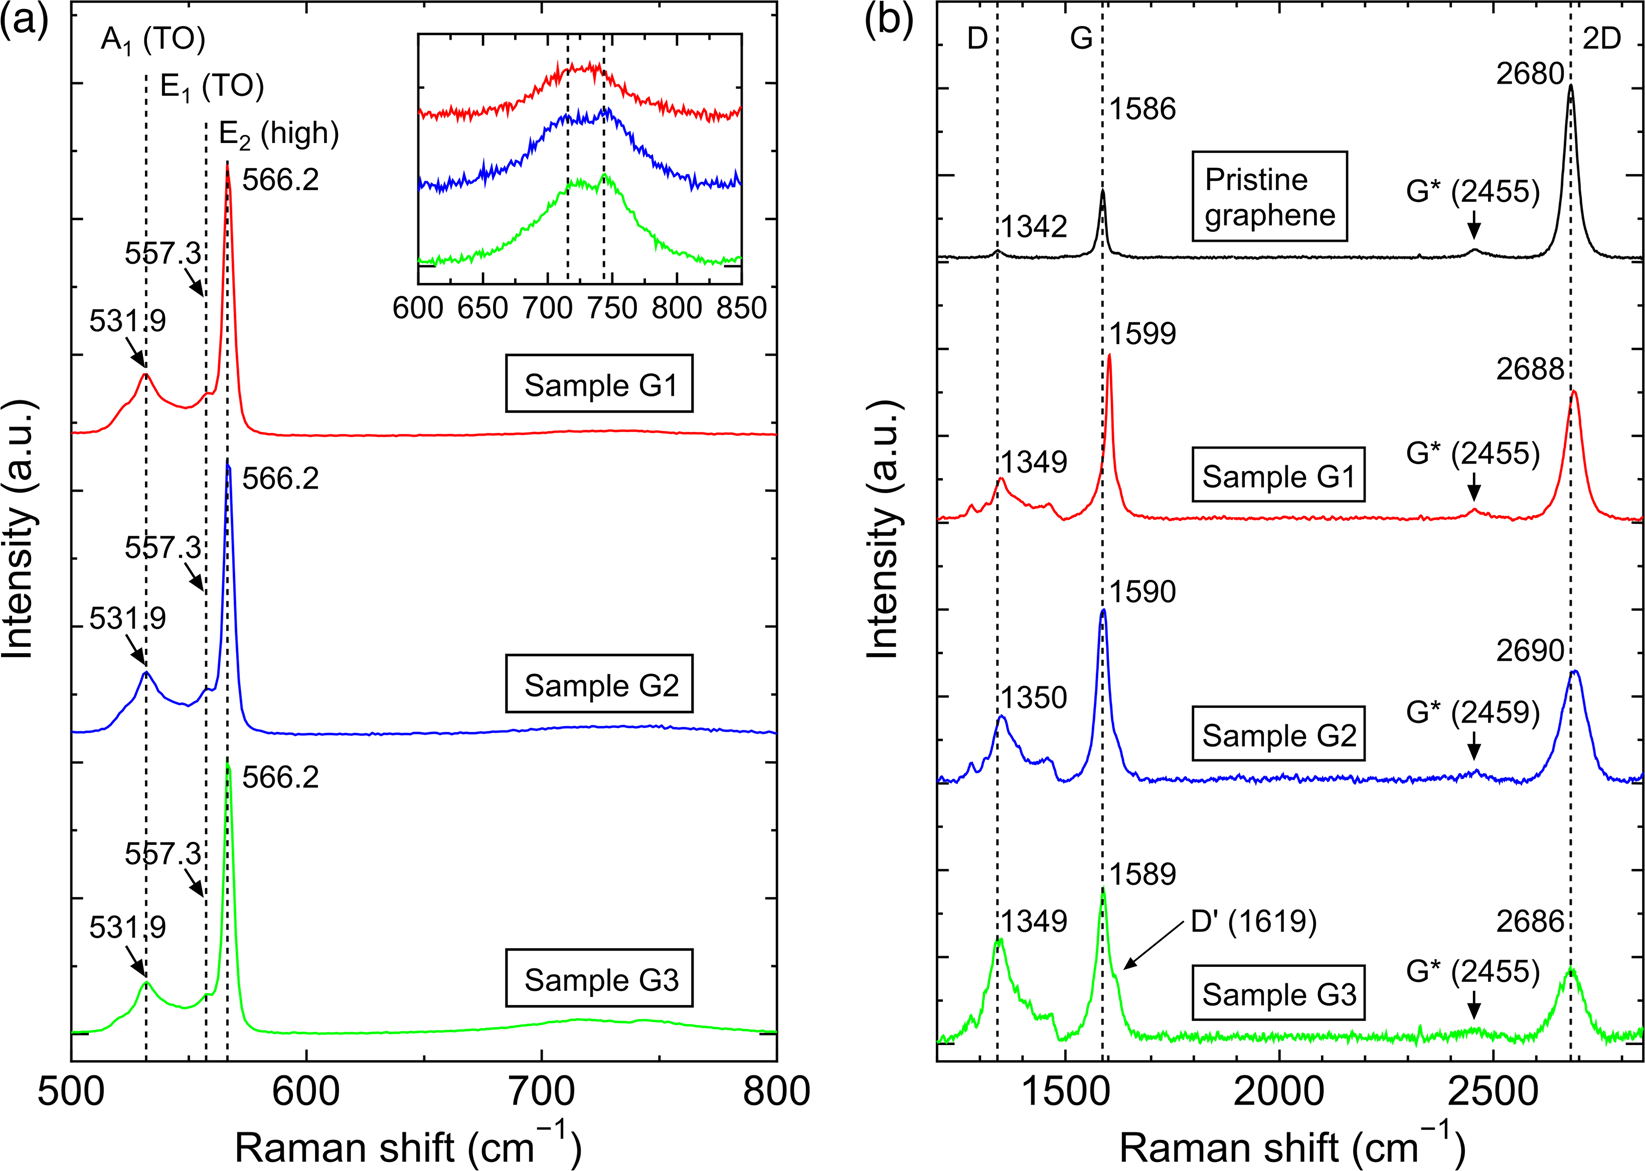
\includegraphics[width=\textwidth]{figures/paper-iv/fig-8.png}
    \caption[Micro-Raman spectroscopy of the nanocolumn samples,\newline including the graphene for each respective sample]{Micro-Raman spectroscopy of the nanocolumn samples, including the graphene for each respective sample. Raman spectra of (\textbf{a}) samples G1, G2 and G3 between 500 and 800 cm\textsuperscript{-1}, with the peak frequencies of the A\textsubscript{1} (TO), E\textsubscript{1} (TO) and E\textsubscript{2} (high) modes indicated by vertical dashed lines (inset: magnification from 600 to 850 cm\textsuperscript{-1}, with the identified peak frequencies at 715 and 743 cm\textsuperscript{-1} of the possible SO and LPP modes, respectively \cite{2016robins,2009jeganathan}, indicated by vertical dashed lines), and (\textbf{b}) pristine graphene, samples G1, G2 and G3 between 1100 and 3200 cm\textsuperscript{-1}. The dashed lines indicate D, G and 2D peak positions of pristine graphene (adapted with permission from ref. \citenum{liudimulyo2020853} \copyright \ Liudi Mulyo \textit{et al}, 2020.}
    \label{fig:figures/paper-iv/fig-8}
\end{figure}

%=======================================================================
%%% References 

\clearpage
\phantomsection
\specialsection
\headerspecialsection

{\hypersetup{urlcolor=ntnu,linkcolor=sophia} % set clickable URL title color to black, not blue like in the main document

\bibliographystyle{unsrtnat-mod} % NATBIB ref style
\bibliography{references}
}

%=======================================================================
%%%% Curriculum vitae

\chapter[Curriculum vitae]{\textsc{Curriculum vitae} \vspace{8pt} \\ Author}

\setcounter{page}{1}
\renewcommand{\thepage}{L-\arabic{page}}

\markboth{Curriculum vitae}%
{Curriculum vitae}

\regularsection
\headerregularsection

% ============================================================================================================

{\color{sophia} \small \bfseries \fontfamily{bch} \selectfont \scshape Personal information} \vspace{4mm}

\noindent Family name, given name \hspace{3mm} : \hspace{2.4mm} Author \\
Nationaliy \hspace{25mm} : \hspace{2.4mm} Citizenship 
\\
Place, date of birth \hspace{13mm} : \hspace{2.4mm} City (Country), Month date\textsuperscript{st/nd/rd/th}, yyyy
\\
Current address \hspace{16.7mm} : \hspace{2.4mm} Address, Postal code City, NO 

% =====================================================

\begin{adjustwidth}{0cm}{1cm}
{\vspace{4mm} \color{sophia} \small \bfseries \fontfamily{bch} \selectfont \scshape Educational background and research experience} \vspace{4mm}
\end{adjustwidth}

\noindent \textbf{Doctor of Philosophy (Ph.D.)} in Electronic Systems\\ Norwegian University of Science and Technology (NTNU), Trondheim, NO\\ month yyyy - month 2021
    \vspace{-0.2cm}
    \begin{itemize}[itemsep=0.7pt, parsep=0.7pt, leftmargin=7mm, label=\adforn{43}] % or alternatively (not rotated), \footnotesize\ding{} 121, 122, 117, 118, 114, 212
        \item Thesis title: The title of PhD thesis
        \item Advisors: Professor Supervisor and Professor Co-supervisor
        \item Additional information, like collaborative researcher at another Laboratory (name of the Professor) at University X, City, Country for total of xx months
    \end{itemize}
    \vspace{0.5mm}
    
\noindent \textbf{Master of Science (M.Sc.)} in Condensed Matter Physics\\ Norwegian University of Science and Technology (NTNU), Trondheim, NO\\ month yyyy - month 2013
    \vspace{-0.2cm}
    \begin{itemize}[itemsep=0.7pt, parsep=0.7pt, leftmargin=7mm, label=\adforn{43}] % or alternatively (not rotated), \footnotesize\ding{} 121, 122, 117, 118, 114, 212
        \item Thesis title: The title of MSc thesis
        \item Advisors: Professor Supervisor and Professor Co-supervisor
    \end{itemize}
    \vspace{0.5mm}
    
\noindent \textbf{Bachelor of Engineering (B.Eng.)} in Engineering Physics\\ Norwegian University of Science and Technology (NTNU), Trondheim, NO\\ month yyyy - month 2010
    \vspace{-0.2cm}
    \begin{itemize}[itemsep=0.7pt, parsep=0.7pt, leftmargin=7mm, label=\adforn{43}] % or alternatively (not rotated), \footnotesize\ding{} 121, 122, 117, 118, 114, 212
        \item Thesis title: The title of BEng thesis
        \item Advisors: Professor Supervisor and Professor Co-supervisor
    \end{itemize}

% ============================================================================================================
\newpage

\begin{adjustwidth}{0cm}{1cm} % 
{\vspace{3mm} \color{sophia} \small \bfseries \fontfamily{bch} \selectfont \scshape Teaching experience} \vspace{3mm}
\end{adjustwidth}

\noindent Laboratory assistant for various courses, at \textbf{NTNU}: Nanoelectronics 2 (spring 2020 \& 2021), Semiconductor Physics with Lab (spring 2017-2020), Physical Methods for Nanostructuring and Characterization (autumn 2017 \& 2018), Chemical Methods for Synthesis and Characterization of Nanomaterial (autumn 2017 \& 2018).

% ============================================================================================================

\begin{adjustwidth}{0cm}{1cm} % 
{\vspace{3mm} \color{sophia} \small \bfseries \fontfamily{bch} \selectfont \scshape Awards} \vspace{1mm}
\end{adjustwidth}

\begin{itemize}[itemsep=0.7pt, parsep=0.7pt, leftmargin=7mm, label=\adforn{43}] % or alternatively (not rotated), \footnotesize\ding{} 121, 122, 117, 118, 114, 212
    \item Norges tekniske h{\o}gskoles fond, a travel grant for \href{http://ece.umich.edu/issled2017/}{ISSLED 2017} \hfill 2017
    \item NorFab travel grant for \href{https://mbe2016.sciencesconf.org/conference/mbe2016/pages/MBE2016_Final_program.pdf#page=42}{MBE 2016} and \href{http://www.csw2017.org}{CSW 2017} \hfill 2017-2018
    \item NorFab project support, for research visit in University X \hfill 2018-2019
    \item PhD scholarship, NTNU \hfill 2017-2021
\end{itemize}

% ============================================================================================================

\begin{adjustwidth}{0cm}{1cm} % 
{\vspace{2mm} \color{sophia} \small \bfseries \fontfamily{bch} \selectfont \scshape Skills} \vspace{3mm}
\end{adjustwidth}

\noindent Scientific (laboratory) competency
\vspace{-0.1cm}
\begin{itemize}[itemsep=0.7pt, parsep=0.7pt, leftmargin=7mm, label=\adforn{43}] % or alternatively (not rotated), \footnotesize\ding{} 121, 122, 117, 118, 114, 212
    \item Experienced with the growth of semiconductor using molecular beam epitaxy technique.
    \item Skilled for material characterization techniques using scanning electron microscopy, photoluminescence, and Raman spectroscopy.
    \item Familiar with device fabrication tools, including mask/maskless aligner, e-beam/sputter deposition, plasma-enhanced chemical vapor deposition, wet etching, and inductively-coupled plasma reactive ion etching. 
    \item Basic knowledge of e-beam lithography and X-ray diffraction.
\end{itemize}

\noindent Computer literacy
\vspace{-0.1cm}
\begin{itemize}[itemsep=0.7pt, parsep=0.7pt, leftmargin=7mm, label=\adforn{43}] % or alternatively (not rotated), \footnotesize\ding{} 121, 122, 117, 118, 114, 212
    \item Microsoft Windows, MacOS, and Debian-based Linux (competent)
    \item Microsoft Office, Inkscape, ImageJ, Ngraph, and \LaTeX \ (intermediate)
    \item SketchUp, Blender, Python, MatLab, \verb!C++!, HTML, and LabView (beginner)
    % (beginner)
\end{itemize}

\noindent Language fluency \\
    \begin{minipage}[t]{.5\linewidth}
        \vspace{-0.2cm}
        \begin{itemize}[itemsep=0.7pt, parsep=0.7pt, leftmargin=7mm, label=\adforn{43}] % or alternatively (not rotated), \footnotesize\ding{} 121, 122, 117, 118, 114, 212
            \item Indonesia (native)
            \item English (full professional)
        \end{itemize}
    \end{minipage}\hspace{0.1cm}
    \begin{minipage}[t]{.4\linewidth}
        \vspace{-0.2cm}
        \begin{itemize}[itemsep=0.5pt, parsep=0.7pt, leftmargin=7mm, label=\adforn{43}] % or alternatively (not rotated), \footnotesize\ding{} 121, 122, 117, 118, 114, 212
            \item Japanese (elementary)
            \item Norwegian (elementary)
        \end{itemize}
    \end{minipage}

% ============================================================================================================

\begin{adjustwidth}{0cm}{1cm} % 
{\vspace{4mm} \color{sophia} \small \bfseries \fontfamily{bch} \selectfont \scshape Contact information} \vspace{3mm}
\end{adjustwidth}

\noindent E-mail \hspace{30.8mm} : \hspace{2.4mm} \href{mailto:author@outlook.com}{author@outlook.com} \\
Homepage \hspace{24.9mm} : \hspace{2.4mm} \href{https://author.github.io}{https://author.github.io}
%%%% Dissemination

\chapter{Dissemination of research}

\setcounter{figure}{0}
\renewcommand{\thefigure}{D.\arabic{figure}}

\updatemylofdissemination

\markboth{Dissemination of research}%
{Dissemination of research}

\regularsection
\headerregularsection

% to be used in the future
% https://tex.stackexchange.com/questions/297365/how-to-use-bibtex-for-putting-a-nice-publication-list-in-resume-with-document-cl
% https://gist.github.com/deparkes/3df4da19de3359dd0a1a59a59f9936cf
% https://tex.stackexchange.com/questions/97057/including-additional-bibliography-publication-list-in-thesis
% https://tex.stackexchange.com/questions/33008/what-is-the-most-convenient-way-to-create-annotated-bibliographies-e-g-in-a-li

% ============================================================================================================

{\color{sophia} \small \bfseries \fontfamily{bch} \selectfont \scshape Publications in peer reviewed journals}

\begin{enumerate}[wide=0em, leftmargin=*, labelsep=0.5em, widest=99, label={[\arabic*]}]

    \item \textbf{Author 1}, Author 2, Author 3, Author 4, Author 5, Author 6, and Author 7. \href{https://doi.org/10.1016/}{Title of the paper}. \textit{Journal of Crystal Growth} \textbf{480}, 67-73 (2017).
    
    \item \textbf{Author 1}, Author 2, Author 3, Author 4, Author 5, Author 6, and Author 7. \href{https://doi.org/10.1088/}{Title of paper 2}. \textit{Nanotechnology} \textbf{30} (1), 015604 (2018). \\
    \textit{This article was chosen as \textbf{cover image/featured article}, see \ref{fig:coverimage}.}
    
    \item Author 1\textcolor{red}{*}, \textbf{{Author 2}\textcolor{red}{*}}, Author 3, Author 4, Author 5, Author 6, Author 7, and Author 8. \href{https://doi.org/10.1021/}{Title of paper 3}. \textit{Nano Letters} \textbf{19} (3), 1649-1658 (2019). \\ \textcolor{red}{\textbf{*equal contributions}}
    
    \item \textbf{Author 1}, Author 2, Author 3, Author 4, Author 5, and Author 6. \href{https://doi.org/10.1038/}{Title of paper 4}. \textit{Scientific Reports} \textbf{10}, 853 (2020).
    
\end{enumerate}
 
{\color{sophia} \small \bfseries \fontfamily{bch} \selectfont \scshape \noindent Manuscript under review}

\begin{enumerate}[wide=0em, leftmargin=*, labelsep=0.5em, widest=99, label={[\arabic*]}]

    \item \textbf{Author 1}, Author 2\textcolor{red}{*}, Author 3\textcolor{red}{*}, Author 4, Author 5, Author 6, Author 7, Author 8, Author 9, and Author 10. \textcolor{ntnu}{Title of manuscript}. \\
    \textcolor{red}{*equal contributions}

\end{enumerate}

\begin{figure}
    \centering
    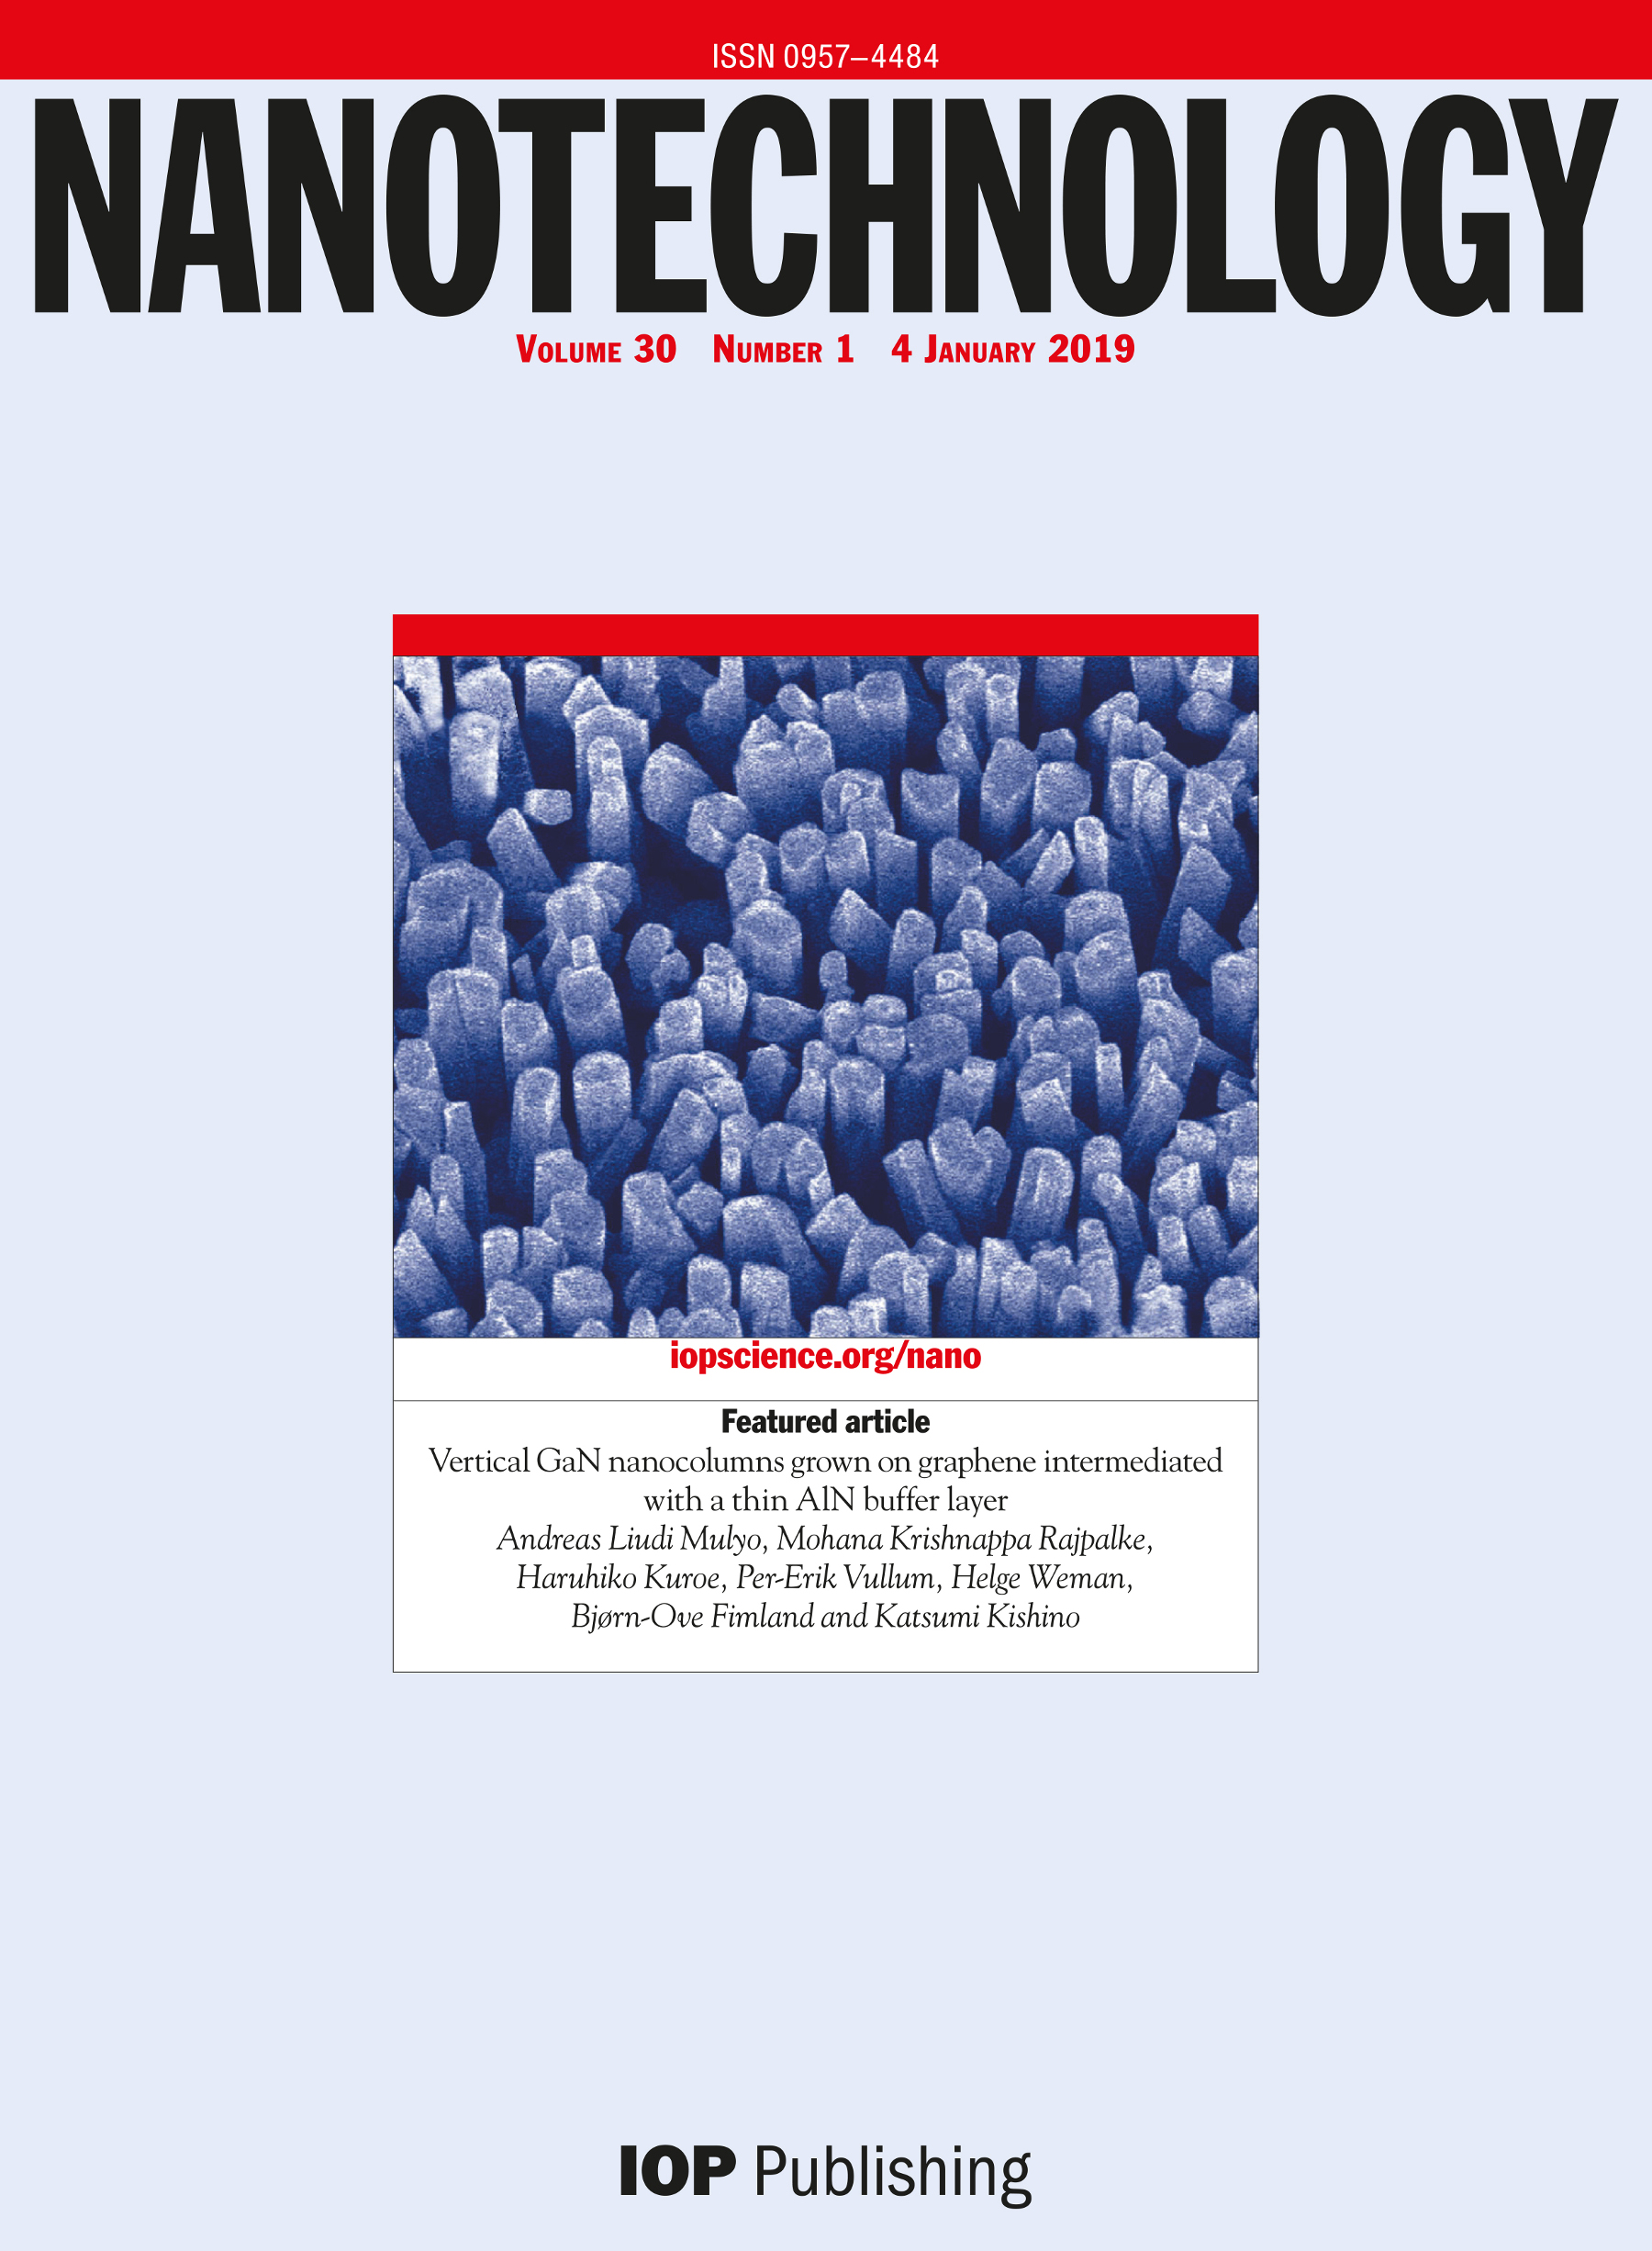
\includegraphics[width=\textwidth]{figures/EN6xzaWWAAEHOBt.jpg}
    \caption[Cover image/featured article in Nanotechnology]{Our work published in Nanotechnology was selected as a cover image/featured article for the first issue of 2019 (4 January).}
    \label{fig:coverimage}
\end{figure}
 
\newpage
 
{\color{sophia} \small \bfseries \fontfamily{bch} \selectfont \scshape \noindent Conference participation (presentations)} \\

\noindent Name of the author with \textsuperscript{\textdagger} indicates the presenter. Half of the past meeting records (i.e., conference websites or pdf files of the conference programs) are still accessible online, and unfortunately half of them are no longer active (as of December 03 2020). For the latter, reader might notice that they are linked via \href{http://web.archive.org}{Internet Archive} or \href{https://author.github.io}{my personal website}.

\begin{enumerate}[wide=0em, leftmargin=*, itemsep=3pt, labelsep=0.5em, widest=99, label={[\arabic*]}]

    \item \textbf{Author 1\textsuperscript{\textdagger}}, Author 2, Author 3, Author 4, Author 5, and Author 6. \textit{Title of the conference}. \textcolor{sophia}{Contributed talk} at \href{https://andreasliudimulyo.github.io/file/past-conferences/ISSLED_2017_Final_Program.pdf#page=17}{The 11th International Symposium on Semiconductor Light Emitting Devices (ISSLED 2017), Banff, Canada, October 08-12 2017}.
    
    \item Author 1\textsuperscript{\textdagger}, \textbf{Author 2}, Author 3, Author 4, Author 5, and Author 6. \textit{Title of the conference}. \textcolor{sophia}{Contributed talk} at \href{https://andreasliudimulyo.github.io/file/past-conferences/2017Nano@NTNU.pdf#page=4}{Nano@NTNU Symposium, Trondheim, Norway, December 06-07 2017}.
    
    \item \textbf{Author 1\textsuperscript{\textdagger}}, Author 2, Author 3, Author 4, Author 5, and Author 6. \textit{Title of the conference}. \textcolor{sophia}{Poster presentation} at \textcolor{ntnu}{Nano@NTNU Symposium, Trondheim, Norway, December 06-07 2017}. \\
    \textit{No website or pdf file of the conference program is associated with this item.}
    
    \item Author 1\textsuperscript{\textdagger}, \textbf{Author 2}, Author 3, Author 4, Author 5, Author 6, Author 7, and Author 8. \textit{Title of the conference}. \textcolor{sophia}{Contributed talk} at \href{https://andreasliudimulyo.github.io/file/past-conferences/NWW2018-Detailed-Preliminary-Program.pdf#page=20}{Nanowire Week, Hamilton, Canada, June 11-15 2018}.
    
    \item Author 1, \textbf{Author 2}, Author 3, Author 4, Author 5, Author 6, Author 7, and Author 8\textsuperscript{\textdagger}. \textit{Title of the conference}. \textcolor{sophia}{Poster presentation} at \href{http://web.archive.org/web/20191029062712/http://www.iwn2018.jp/IWN_AP_including_late_news.pdf#page=123}{ The International Workshop on Nitride Semiconductors, Kanazawa, Japan, November 11-16 2018}.
    
    \item \textbf{Author 1}, Author 2, Author 3, Author 4, Author 5, Author 6\textsuperscript{\textdagger}, and Author 7. \textit{Title of the conference}. \textcolor{sophia}{Poster presentation} at \href{http://web.archive.org/web/20191029062712/http://www.iwn2018.jp/IWN_AP_including_late_news.pdf#page=155}{ The International Workshop on Nitride Semiconductors, Kanazawa, Japan, November 11-16 2018}.

    \begin{sloppypar}
    \item \textbf{Author 1\textsuperscript{\textdagger}}, Author 2, Author 3, Author 4, Author 5, Author 6, and Author 7. \textit{Title of the conference}. \textcolor{sophia}{Contributed talk} at \href{http://www.nano-network.net/wp-content/uploads/2019/06/Preliminary-program-Workshop.pdf}{ The 10th annual workshop of Norwegian PhD Network on Nanotechnology for Microsystems, Tromsø, Norway, June 17-19 2019}.
    \end{sloppypar}
    
    \item \textbf{Author 1}, Author 2, Author 3, Author 4, Author 5, and Author 6\textsuperscript{\textdagger}. \textit{Title of the conference}. \textcolor{sophia}{Poster presentation} at \href{https://andreasliudimulyo.github.io/file/past-conferences/icns-13-program-web.pdf#page=9}{The 13th International Conferences on Nitride Semiconductors, Bellevue, Washington (Seattle), USA, July 07-12 2019}.
    
\end{enumerate}
%%%% Copyright permissions

\chapter[Copyright permissions]{Copyright permissions}

\markboth{Copyright permissions}%
{Copyright permissions}

\regularsection
\headerregularsection

Below is the complete list of the copyright figures shown in this Doctoral thesis, mainly from chapter 1 to chapter 4.

\begin{itemize} [wide=0em, leftmargin=*, label=\adforn{74}] % , itemsep=0.7pt, parsep=0.7pt, label=\small\ding{110} 121, 122, 117, 118, 110, 111, 113, 114, 212]

    % \bibliographystyle{unsrtnat-mod}
    % \nobibliography{references}
    
    % % https://tex.stackexchange.com/questions/129811/file-ended-error-when-using-nobibliography
    % % https://tex.stackexchange.com/questions/142985/using-bibentry-to-insert-reference-in-text-and-omit-the-list-of-references-at-th
    % % https://tex.stackexchange.com/questions/33008/what-is-the-most-convenient-way-to-create-annotated-bibliographies-e-g-in-a-li
    
    % % i don't understand why it does not work here, especially with the similar pattern as of last point
    % % in any case, if it the code works, it will display "cit. on p." (or other declaration in the PREMABLE), which is unwanted here. So, manual is the only way.
    % % this will be used only for comparison
    % % UPDATE 20201211:
    % % it seems that bibentry does not work properly (annoying error messages) when the bibentry is used in the main text (in condition where backref of hyperref is activated).
    % % see:
    % % https://comp.text.tex.narkive.com/x2PWbp7j/backref-and-bibentry-conflict
    % % possible way to solve, but I can't implement them: 
    % % http://qianglee.blogspot.com/2006/08/make-bibentry-compatible-with-backref.html

    \item \ref{fig:figures/paper-iv/fig-1}\mynote{\pcol{page} \colpageref{fig:figures/paper-iv/fig-1}}is adapted with permission from: \\ A. Liudi Mulyo. \href{https://www.nature.com/articles/s41598-019-55424-z}{The influence of AlN buffer layer on the growth of self-assembled GaN nanocolumns on graphene}. \textit{Scientific Reports} \textbf{10}, 853 (2020). \\ Copyright \copyright \ 2020 Liudi Mulyo.
    
    \item \ref{fig:figures/paper-iv/fig-2}\mynote{\pcol{page} \colpageref{fig:figures/paper-iv/fig-2}}is adapted with permission from: \\ A. Liudi Mulyo. \href{https://www.nature.com/articles/s41598-019-55424-z}{The influence of AlN buffer layer on the growth of self-assembled GaN nanocolumns on graphene}. \textit{Scientific Reports} \textbf{10}, 853 (2020). \\ Copyright \copyright \ 2020 Liudi Mulyo.
    
    \item \ref{fig:figures/paper-iv/fig-3}\mynote{\pcol{page} \colpageref{fig:figures/paper-iv/fig-3}}is adapted with permission from: \\ A. Liudi Mulyo. \href{https://www.nature.com/articles/s41598-019-55424-z}{The influence of AlN buffer layer on the growth of self-assembled GaN nanocolumns on graphene}. \textit{Scientific Reports} \textbf{10}, 853 (2020). \\ Copyright \copyright \ 2020 Liudi Mulyo.
    
    \item \ref{fig:figures/paper-iv/fig-4}\mynote{\pcol{page} \colpageref{fig:figures/paper-iv/fig-4}}is adapted with permission from: \\ A. Liudi Mulyo. \href{https://www.nature.com/articles/s41598-019-55424-z}{The influence of AlN buffer layer on the growth of self-assembled GaN nanocolumns on graphene}. \textit{Scientific Reports} \textbf{10}, 853 (2020). \\ Copyright \copyright \ 2020 Liudi Mulyo.

    \item \ref{fig:figures/paper-iv/fig-5}\mynote{\pcol{page} \colpageref{fig:figures/paper-iv/fig-5}}is adapted with permission from: \\ A. Liudi Mulyo. \href{https://www.nature.com/articles/s41598-019-55424-z}{The influence of AlN buffer layer on the growth of self-assembled GaN nanocolumns on graphene}. \textit{Scientific Reports} \textbf{10}, 853 (2020). \\ Copyright \copyright \ 2020 Liudi Mulyo.

    \item \ref{fig:figures/paper-iv/fig-6}\mynote{\pcol{page} \colpageref{fig:figures/paper-iv/fig-6}}is adapted with permission from: \\ A. Liudi Mulyo. \href{https://www.nature.com/articles/s41598-019-55424-z}{The influence of AlN buffer layer on the growth of self-assembled GaN nanocolumns on graphene}. \textit{Scientific Reports} \textbf{10}, 853 (2020). \\ Copyright \copyright \ 2020 Liudi Mulyo.

    \item \ref{fig:figures/paper-iv/fig-7}\mynote{\pcol{page} \colpageref{fig:figures/paper-iv/fig-7}}is adapted with permission from: \\ A. Liudi Mulyo. \href{https://www.nature.com/articles/s41598-019-55424-z}{The influence of AlN buffer layer on the growth of self-assembled GaN nanocolumns on graphene}. \textit{Scientific Reports} \textbf{10}, 853 (2020). \\ Copyright \copyright \ 2020 Liudi Mulyo.
        
\end{itemize}
%%% Index

\cleardoublepage\phantomsection % to fix wrong hyperref to \chapter*{print index}
% \setcounter{page}{1}
% \renewcommand{\thepage}{I-\arabic{page}}

% \markboth{Index}% not necessary for "\renewenvironment{theindex} % require"
% {Index}

% \regularsection % not necessary as there is no section and subsection here

\setcounter{page}{1}
\renewcommand{\thepage}{M-\arabic{page}}

% ==============================

\headerregularsection % it appears that "index" has a function of "\Makeuppercase" within their heading/footer. so to solve this, in practice, it is similar with reference, meaning the same way to tackle this: by issuing "\headerspecialsection"

% % OR

% \headerspecialsection % not necessary (?) for "\renewenvironment{theindex} % require"

% % err.... after several runs, the header/footer for "index" is slightly bit complicated 
% % you need to run a few times to see the changes
% % these two functions are not completely useless

% ==============================

% % run with "\renewenvironment{theindex} % require "\chapter{Index} \begin{multicols}{2} \printindex \end{multicols}" in the preamble
% \chapter{Index} 
% \begin{multicols}{2}
% \printindex
% \end{multicols}

% % OR

% run with "\renewenvironment{theindex} % require only "\printindex" in the backmatter/index.tex" in the preamble
{\hypersetup{linkcolor=sophia}
\printindex
}
% Multi-column with "\renewenvironment{theindex}" in the preamble : https://latex.org/forum/viewtopic.php?t=1735
% other alternatives are available there too

% how to index
% https://withoutbullshit.com/blog/the-sublime-joy-of-making-a-book-index-indexing
% https://writingcooperative.com/five-step-process-for-writing-a-book-index-9e2e5d763302

% to-do list in the future:
% thumb indices --> https://data.math.au.dk/latex/bog/version3/beta/ltxb-2011-09-13-20-10.pdf#page=459
% first and last word in the header --> https://tex.stackexchange.com/questions/26122/indexing-an-interval-of-words-on-top-of-every-page

% \cleardoublepage % intentionally put Colophon in the even page -> ignore the following error
% % "Package marginnote Warning: Consecutive odd pages found. Note, it is not recommended to use consecutive odd pages in a double-ended document. The pages of your document should always be a sequence: odd-even-odd-even-... Maybe you've forgotten a \cleardoublepage before changing the page numbering on page End-1."
%\pagestyle{empty}

\setcounter{page}{1}
\renewcommand{\thepage}{End-\arabic{page}}

\hfill

\vfill

{

\begin{adjustwidth}{-1mm}{1cm} % 
{\noindent \color{sophia} 
\small
\bfseries \fontfamily{bch} \selectfont \scshape Colophon} \vspace{4mm}
\end{adjustwidth}

\noindent This thesis was typeset using \LaTeX \ and the \texttt{book} documentclass. Main text is contained within the dimension of 115 mm (width)/197.2 mm (length), where the horizontal (top:bottom) and vertical (left:right) margin ratios are 1:1. The width of the margin notes is 12 mm. Style of this thesis is inspired by Friedrich Wiemer's thesis \textit{Security Arguments and Tool-based Design of Block Ciphers} [\url{https://hss-opus.ub.rub.de/opus4/frontdoor/deliver/index/docId/7044/file/diss.pdf}]. \\

\noindent Sebastian Kosch's \textit{Crimson} [\url{https://github.com/skosch/Crimson}] is set as the running text (11 pt) typeface. Matthew Carter’s \textit{Charter} acts as the title (14.4 pt), section (10 pt), subsection (10 pt), and header (8 pt) typefaces. Hermann Zapf's \textit{Palatino} serves as the page (9 pt) typeface. Christian Robertson's \textit{Roboto} [\url{https://tug.org/FontCatalogue/roboto/}] is utilized for the figure caption (8 pt) typeface. Libertine Open Fonts Project's \textit{Linux Libertine} [\url{https://tug.org/FontCatalogue/linuxlibertine/}] and Linus Romer's \textit{Miama Nueva} [\url{https://tug.org/FontCatalogue/miamanueva/}] are used for math/equation (11 pt) and calligraphical (14.4 pt) typefaces. The \texttt{textgreek} package [\url{https://www.ctan.org/pkg/textgreek}] provides Greek letters in normal font (being not \textit{italicized} as in \texttt{\$math\$} mode). \\

\begin{sloppypar}
\noindent Six different color palettes exploited throughout this thesis are listed as follows: \colorbox{ntnu}{\textcolor{White}{\texttt{RGB: 0, 80, 158}}} , \colorbox{sophia}{\textcolor{White}{\texttt{RGB: 125, 0, 45}}} , \colorbox{abstractback}{\texttt{RGB: 255, 248, 220}} , \colorbox{Test}{\texttt{RGB: 231, 231, 231}} , \colorbox{heidelberg}{\textcolor{White}{\texttt{RGB: 0, 65, 120}}} , and \colorbox{Test3}{\textcolor{White}{\texttt{RGB: 128, 128, 128}}} . \\
\end{sloppypar}

\noindent The references were processed by \texttt{BibTeX/natbib} -backref option enabled- with modified \texttt{unsrtnat} bibliography style. Further details on the packages utilized to make this thesis, along with the \LaTeX \ source (template) of this thesis can be found on \url{https://andreasliudimulyo.github.io/#latex}. \\

\begin{sloppypar}
\noindent Most of the graphics in this thesis were generated using \texttt{Inkscape} [\url{https://inkscape.org}] and \texttt{Ngraph} [\url{https://forest.watch.impress.co.jp/library/software/ngraph/}].
\end{sloppypar}

\vspace{4mm}

\noindent\emph{Final Version} as of \today \ at \ \currenttime. 
}

\end{document}
